\documentclass[polish,12pt]{aghthesis}

% Szablon przystosowany jest do druku dwustronnego. 

\usepackage[utf8]{inputenc}
\usepackage{url}
\usepackage{graphicx}
\usepackage{enumerate}
\usepackage{array}
\usepackage{amsmath}
\usepackage{float}
\usepackage{placeins}
\usepackage[export]{adjustbox}
\usepackage{enumitem}
\usepackage{multirow}
\usepackage{longtable}
\usepackage{subcaption}

\graphicspath{ {./images/} }

\author{Emilia Majerz, Aleksandra Pasternak}

\titlePL{System do analizy uszkodzeń poszycia statków powietrznych wykorzystujący konwolucyjne sieci neuronowe}
\titleEN{System for analyzing damage to the surface of aircraft structures using convolutional neural networks}

\fieldofstudy{Informatyka}

\supervisor{prof.\ dr hab.\ inż.\ Witold Dzwinel}

\date{\the\year}


\begin{document}

\maketitle

\newpage

\tableofcontents

\newpage

\section{\SectionTitleProjectVision}
\label{sec:cel-wizja}
\par Rozdział stanowi wprowadzenie do dziedziny problemu, wskazuje cel podjętych prac oraz ich motywację. W tej części pracy można znaleźć ogólny zarys pierwszego planu dla powstałego produktu, a także zapoznać się z już istniejącymi podejściami do podobnych problemów.

\subsection{Charakterystyka problemu}
\par
W trakcie eksploatacji samoloty narażone są na spowodowane korozją uszkodzenia poszycia. Monitorowanie stanu nitów, wchodzących w jego skład, jest jedną z kluczowych operacji podczas sprawdzania zdatności maszyn do lotów. 
\par
Jednym z głównych procesów kontroli, w fazie produkcyjnej oraz przy późniejszej konserwacji, są oględziny, które stanowią ponad 80\% wszystkich przeprowadzanych przeglądów. Oględziny dostarczają informacji o ogólnym stanie maszyny i jej zdatności do lotu, pozwalają wykryć błędy produkcyjne oraz defekty w ich początkowej fazie.
Początkowo, w celu sprawdzenia stanu poszyć, były one analizowane wizualnie przez specjalistów, a następnie poddawane szczegółowym inspekcjom. 
W tradycyjnej metodzie poszycia badane są przez inspektorów, którzy przy pomocy narzędzi takich jak latarki, lustra czy boroskopy wyszukują pęknięcia, fragmenty zajęte rdzą oraz inne uszkodzenia. Dzięki wykorzystaniu podstawowych przyrządów procedura jest tania, jednak czasochłonna. Skuteczność tej metody jest dyskusyjna\cite{repSpencer}, głównie ze względu na błędy ludzkie powodowane np. zmęczeniem\cite{artLock} oraz czynniki zewnętrzne m.in. temperaturę czy oświetlenie.
\par
Wolne od tego typu błędów są systemy automatyczne jak D-Sight. Metoda D-Sight wykorzystuje zjawisko podwójnego odbicia światła od badanej powierzchni. W układzie znajdują się: źródło światła, aparat, ekran odblaskowy oraz badany fragment (w przypadku słabego odbicia światła przez powierzchnię zostaje ona pokryta cienką warstwą płynu). (Rysunek \ref{fig:shemat-dzialania}) 
\begin{figure} [h]
  \centering
  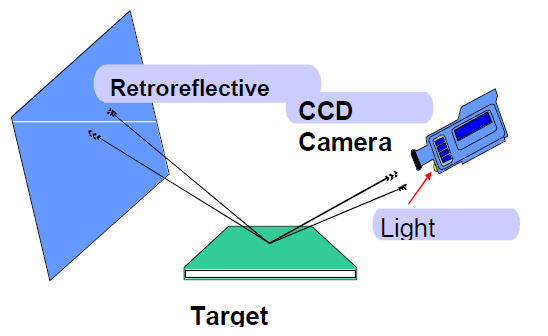
\includegraphics[width=10cm]{images/schemat-dzialania.PNG}
  \caption{Schemat działania systemu D-Sight\cite{artKom}}
  \label{fig:shemat-dzialania}
\end{figure}
\newline
Światło odbija się od analizowanego elementu i pada na ekran odblaskowy składający się z wielu na wpół posrebrzanych szklanych koralików. Ekran ma za zadanie odbić z powrotem wiązki światła pod tym samym kątem do badanej powierzchni, jednak ze względu na niedokładność odbicia wiązki uzyskujemy stożek - efekt D-Sight. Po ponownym odbiciu od poszycia odbłyski zostają zarejestrowane przez aparat znajdujący się ponad źródłem światła. W przypadku, gdy badana powierzchnia jest płaska, co wskazywałoby na brak uszkodzeń, obraz z aparatu pokaże równomierne natężenie światła na całej powierzchni. Odkształcenia z kolei będą skutkować różnicami intensywności na uzyskanym zdjęciu. W technice D-Sight zniekształcenia powierzchni są przekształcane na lokalne zmiany natężenia światła\cite{artRey}.
\begin{figure} [h]
  \centering
  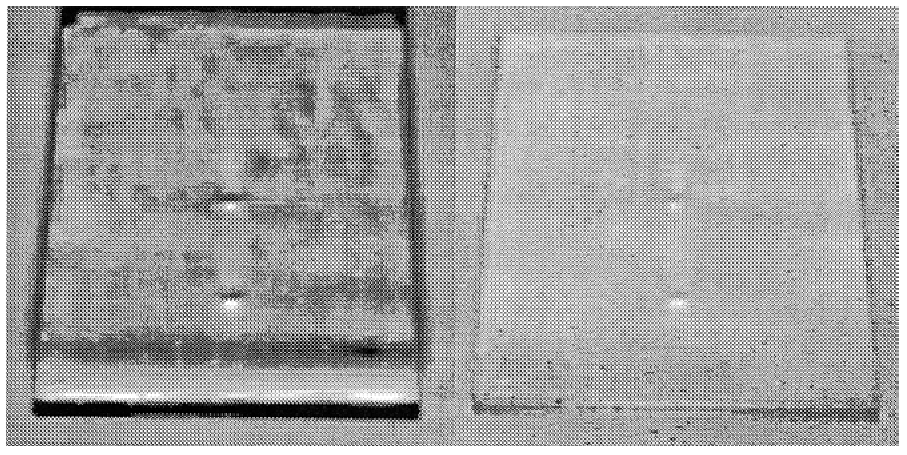
\includegraphics[width=10cm]{images/d-sight-example.PNG}
  \caption{Zdjęcia uzyskane metodą D-Sight\cite{confpaperHeida}}
  \label{fig:d-sight-ex}
\end{figure}
\par
W Polskich Siłach Powietrznych od ponad dwudziestu lat do analizy uszkodzeń stosuje się system DAIS (D-Sight Aircraft Inspection System), który umożliwia wykonanie zdjęć poszycia, ułatwiających wykrycie uszkodzeń. Nadal jednak muszą być one analizowane przez specjalistów, przez co proces jest wciąż wielogodzinny i podatny na błędy ludzkie.

\begin{figure}[h!]
    \begin{adjustbox}{minipage=1.0\paperwidth, pagecenter}
    \centering
    \subfloat[\centering zdjęcie wykonane przez DAIS]{{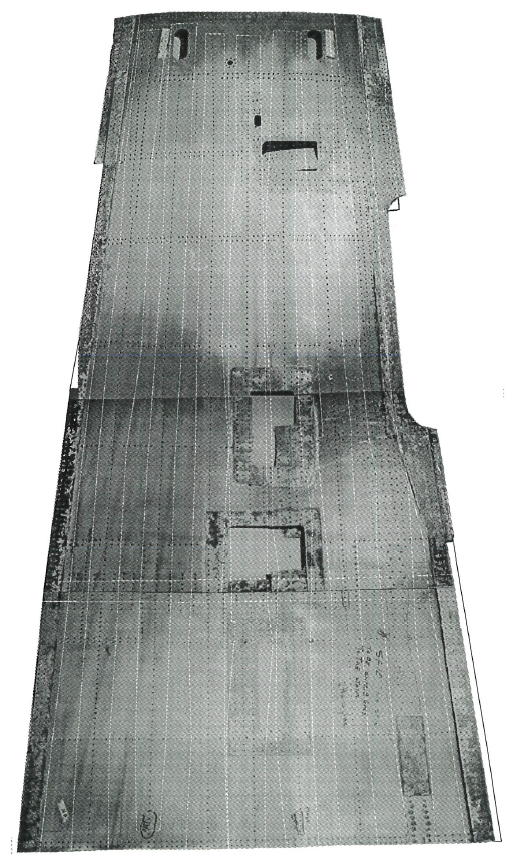
\includegraphics[width=9.9cm, height=15cm]{images/dais-orig.PNG} }}%
    \qquad
    \subfloat[\centering analiza dokonana przez inspektora]{{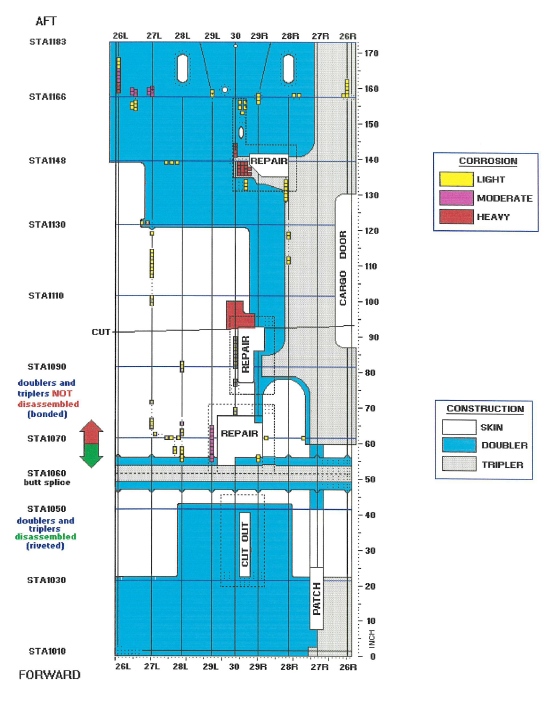
\includegraphics[width=9.9cm, height=15cm]{images/dais-analiza.PNG} }}%
    \end{adjustbox}
    \caption{Poszycie statku powietrznego Boeing 727\cite{repGould}}
    \label{fig:boeing}
\end{figure}

\par
Odpowiedzią na powyższy problem może być zautomatyzowanie procesu oceny stanu poszycia poprzez stworzenie systemu analizującego zdjęcia zrobione przy pomocy systemu DAIS. Dodatkowo, system taki oprócz kwalifikowania nitów do odpowiedniej kategorii w zależności od ich stanu, mógłby również lokalizować uszkodzenia.

\subsection{Motywacja projektu}
Katedra Informatyki uzyskała od Instytutu Technicznego Wojsk Lotniczych dostęp do bazy systemu DAIS, zawierającej ponad pół miliona fotografii fragmentów poszyć samolotów, z których w pracy wykorzystane zostało około 13 tysięcy.
\par
Korozja jest poważnym zagrożeniem, ponieważ narusza spójność poszyć statków i powiązaną z nią zdolność do lotu. Inspekcja struktur pod kątem występowania korozji, przeprowadzana przez specjalistów, jest czasochłonna i kosztowna. Mimo przeszkolenia oraz doświadczenia osób przeprowadzających analizę, może być również zawodna. Od jakości przeprowadzonej kontroli zależy bezpieczeństwo pasażerów maszyn powietrznych oraz otoczenia. O realności problemu uświadomił przemysłowi lotniczemu incydent linii lotniczych Aloha Airlines z 1988 roku, w którym korozja i inne uszkodzenia nitów doprowadziły do zerwania znacznej części poszycia kadłuba Boeinga 737. 
\begin{figure} [h!]
  \centering
  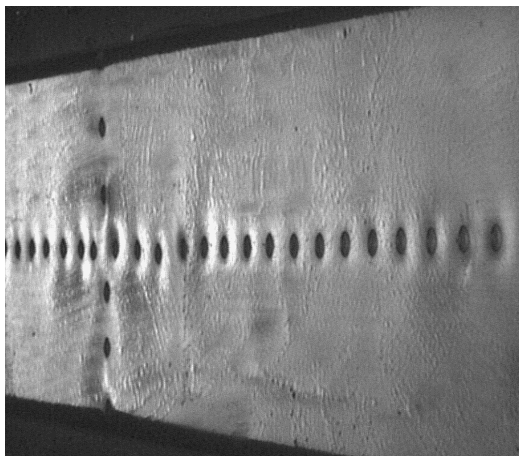
\includegraphics[width=10cm, height=8cm]{images/dais-agh.PNG}
  \caption{Przykładowe zdjęcie z bazy uzyskanej przez AGH}
  \label{fig:dais-agh}
\end{figure}
\par
Postęp technologiczny umożliwia dziś analizę obrazów przez programy komputerowe. Wykorzystanie technologii do oceny stanu poszyć statków powietrznych, wykorzystując zdjęcia zrobione przy pomocy systemu DAIS, pozwoliłoby na znaczne przyspieszenie tego procesu.

\subsection{Wizja produktu}
\par
Oczekiwanym produktem jest system do rozpoznawania korozji na podstawie dostarczonego zdjęcia poszycia.
\par
System powinien usprawniać proces analizy poszycia statków powietrznych pod kątem korozji i zastępować pracę specjalistów, dokonując skutecznej klasyfikacji. Przeznaczony jest on do użytku osób związanych z przemysłem lotniczym, szczególnie z konserwacją maszyn. Dane wejściowe dla produktu stanowią zdjęcia z systemu DAIS.
\par
System obejmuje moduł programowy do klasyfikacji zdjęć oraz umożliwiającą interakcję z nim aplikację webową. Obecność korozji powinna być rozpoznawana przez wcześniej wytrenowaną sieć neuronową. System ma za zadanie przyjąć zdjęcie w formie elektronicznej, przeprowadzić analizę i na jej podstawie zwrócić wynik określający postęp korozji zawierający się w 2-stopniowej skali: korozja - brak korozji. Pożądaną opcją jest również dostarczenie informacji dotyczących fragmentów zdjęcia odpowiadających za daną predykcję.
\vspace{5mm}
\newline Zarys wymagań:
\begin{enumerate}
    \item Określenie stopnia postępu korozji w 2-stopniowej skali: korozja - brak korozji
    \item Stworzenie aplikacji umożliwiającej proste i intuicyjne korzystanie z klasyfikatora
    \item Dostarczenie informacji o pikselach odpowiedzialnych za predykcję
\end{enumerate}
Założenia:
\begin{enumerate}
    \item Zrealizowanie osobnego modułu do klasyfikacji
    \item Przekształcenie danych do formatu odpowiedniego dla sieci
    \item Wykorzystanie do analizy nowoczesnych architektur sieci neuronowych, przeznaczonych do analizy obrazów
    \item Stworzenie interfejsu z wypisanym wynikiem analizy korozji oraz wyświetlonym zdjęciem z zaznaczonym obszarem głównie odpowiadającym za daną predykcję
\end{enumerate}


\subsection{Przegląd istniejących rozwiązań}
\par
Kosztowność, czasochłonność i zawodność metod opartych na wizualnej analizie zdjęć poszycia przez specjalistów, a także szczególnie widoczny w ostatnich latach rozwój technologiczny, zapoczątkowały poszukiwanie zautomatyzowanych sposobów realizacji tego procesu. Aktualnie istniejące metody można podzielić na dwie kategorie: metody oparte o heurystyki oraz metody wykorzystujące uczenie maszynowe. Te pierwsze szeroko wykorzystują możliwości preprocessingu obrazów, poddając je różnym modyfikacjom, takim jak detekcja krawędzi, zmiana wartości pikseli przy wykorzystaniu progowania, czy transformaty. Takie przekształcenia pomagają wyodrębnić cechy dotyczące koloru lub tekstury badanego segmentu, które dalej mogą zostać zaaplikowane do heurystyk, zdolnych do zwracania informacji o uszkodzeniach. 
\begin{figure}[ht]
    \centering
    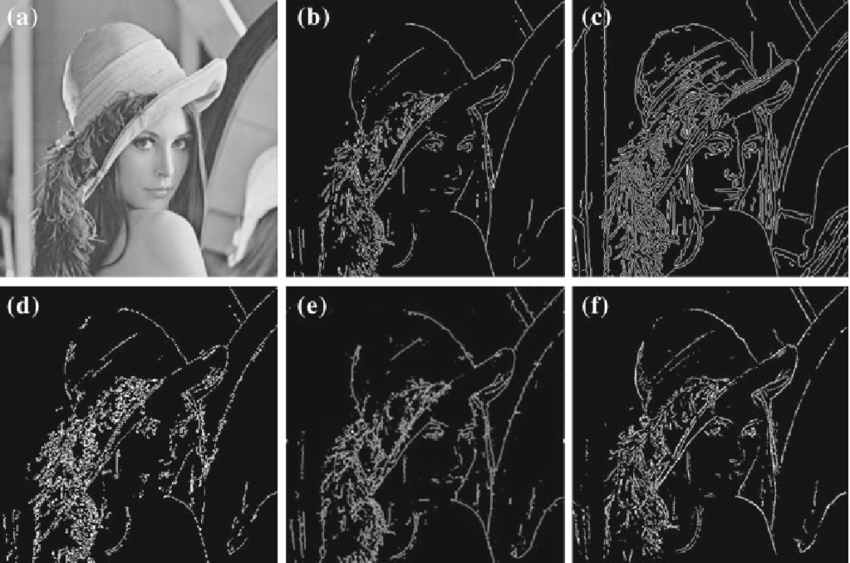
\includegraphics[width=10cm]{images/Lena.png}
    \caption{Przykładowy rezultat metody Canny'ego detekcji krawędzi\cite{artLena}}
    \label{fig:lena}
\end{figure}
\par
Przytoczone podejście do problemu zostało wykorzystane przez naukowców Lee, Chang i Skibniewskiego, którzy wykorzystali analizę kanałów zdjęć: czerwonego, zielonego i niebieskiego do wyodrębnienia cech, których następnie użyli w funkcji pozwalającej na detekcję obecności rdzy na stalowych mostach\cite{artSkib}. Naukowcy Wang i Cheng wykorzystali transformatę Hougha w wersji pozwalającej na detekcję okręgów do znajdowania korozji wżerowej, która to metoda pozwoliła osiągnąć ponad 95\% skuteczności\cite{artWang}. 
\begin{figure}[ht]
    \centering
    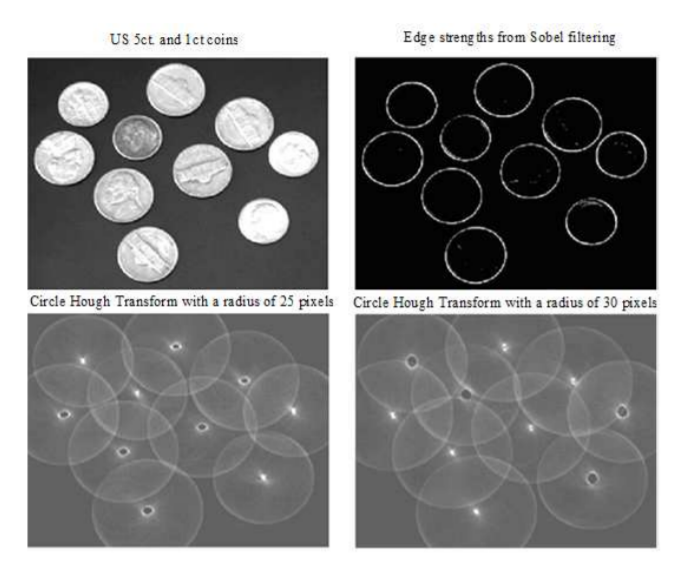
\includegraphics[width=10cm]{images/hough.PNG}
    \caption{Przykład działania transformaty Hougha - jasne punkty na dwóch dolnych zdjęciach pokazują środki wykrytych okręgów dla danej wartości promienia\cite{artHough}}
    \label{fig:hough}
\end{figure}
\par
Pierwotne podejście do tego problemu z użyciem uczenia maszynowego wykorzystywało do tworzenia algorytmów klasyfikujących cechy wyodrębnione z obrazów przy pomocy inżynierii cech. Przykładowo, naukowcy Hoang i Tran zastosowali SVM oraz przesuwane okno do lokalizacji korozji na powierzchni rur\cite{artHoang}. 
\par
Jakość obu przytoczonych rozwiązań jest jednak mocno zależna od jakości wyobrębnionych cech. Sam proces poszukiwania cech jest również trudny do przeprowadzenia, a w przypadku wielu możliwych defektów poszycia udane przedstawienie każdego z nich jako funkcji wyodrębnionych cech staje się niezwykle skomplikowane. Kolejnych trudności może przysporzyć próba przedstawienia złożonych uszkodzeń za pomocą elementarnych cech obrazu.
\par
Rozwiązaniem dla powyższych problemów może być zyskująca w ostatnich latach coraz większą popularność gałąź uczenia maszynowego - uczenie głębokie. Sieci neuronowe nie wymagają dostarczania im przygotowanych cech - są one w stanie nauczyć się tych cech same, dostając na wejściu zdjęcie. Dla danych w postaci obrazu aktualnie wykorzystywanym typem sieci neuronowych są sieci konwolucyjne. Sieci takie posiadają w swojej strukturze specjalne warstwy (filtry) konwolucyjne, pozwalające na skuteczne ekstrahowanie cech obrazu przy jednoczesnym zmniejszeniu liczby koniecznych do wyuczenia wag względem sieci posiadających wyłącznie warstwy gęste.
\par
Ze względu na swoją skuteczność w zadaniach dotyczących klasyfikacji obrazów, sieci konwolucyjne (oraz bazujące na filtrach konwolucyjnych bardziej skomplikowane architektury sieci neuronowych) uważane są za \textit{state of the art} w tej dziedzinie. Zostały one już z powodzeniem wykorzystane w zadaniach dotyczących detekcji uszkodzeń powierzchni. Należy jednak pamiętać, że to podejście wymaga bardzo dużych rozmiarów zbiorów danych - min. 1000 zdjęć przeznaczonych do treningu dla każdego rodzaju uszkodzenia.
\par
Naukowcy Li, Huang, Xie, Yao i Chen wykorzystali sieć konwolucyjną oraz sieć SSD do detekcji uszkodzeń powierzchni, osiągając 95\% poprawnych detekcji\cite{artLi}. Naukowcy Cha oraz Choi wykazali, że wykorzystanie 5-warstwowej sieci konwolucyjnej pozwala na osiągnięcie 98\% skuteczności w detekcji uszkodzeń\cite{artCha1}.
\par
Mówiąc stricte o analizie poszyć statków powietrznych, a nie analizie powierzchni w ogóle, liczba istniejących rozwiązań znacznie spada. Gunatilake, Siegel, Jordan i Podnar zaproponowali system bazujący na mobilnej platformie służacej do generowania zdjęć w czasie rzeczywistym, złożony także z konsoli umożliwiającej podgląd zdjęć oraz z biblioteki do przetwarzania obrazów i z algorytmów przygotowanych w celu detekcji uszkodzeń poszycia samolotów\cite{artSiegel}. System umożliwia zaznaczanie różnego rodzaju uszkodzeń poprzez interakcję z GUI, w którym inspektor może aplikować dedykowane filtry, dostosowując ich intensywność w zależności od potrzeb.
\begin{figure}[ht]
    \centering
    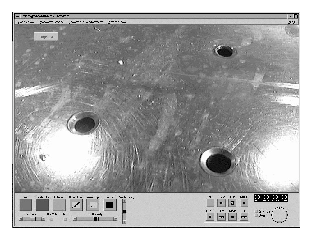
\includegraphics[width=10cm]{images/console.png}
    \caption{GUI proponowane w systemie Gunatilake i in.\cite{artSiegel}}
    \label{fig:IIW-console}
\end{figure}
Ten system nie udostępnia jednak możliwości automatycznej klasyfikacji obrazów. W kolejnej\cite{artSiegel2} publikacji Gunatilake i Siegel proponują algorytmy do detekcji uszkodzeń mechanicznych poszycia oraz korozji, silnie wykorzystujące inżynierię cech, a w ostatnim etapie uczenie maszynowe - niewielką sieć neuronową (1 warstwa ukryta) do klasyfikacji uszkodzeń (72\% skuteczności) oraz algorytm 1-nearest-neighbour do klasyfikacji korozji (wykrywający 95\% skorodowanych powierzchni ze zbioru testowego).
\par
Naukowcy Malekzadeh, Abdollahzadeh, Nejati i Cheung\cite{artMalekzadeh} wykorzystali konwolucyjne sieci neuronowe do wyodrębnienia cech obrazów, które następnie zostały sklasyfikowane przy użyciu SVM. Przeprowadzone przez autorów doświadczenia wykazały, że najlepiej spisującą się siecią spośród testowanych była sieć VGG-F. W celu skrócenia czasu przetwarzania obrazu wykorzystany został detektor SURF, wskazujący fragmenty zdjęcia podejrzane o zawieranie defektów. Powyższe podejście pozwoliło uzyskać 96-procentową skuteczność na nowych obrazach. 
\begin{figure}[ht]
    \centering
    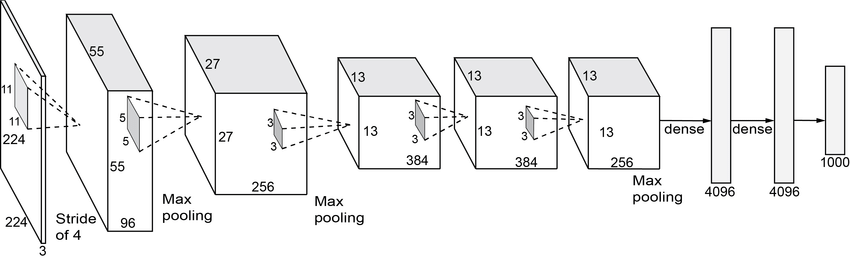
\includegraphics[width=12cm]{images/vgg-f.png}
    \caption{Architektura sieci VGG-F\cite{artVggf}}
    \label{fig:vgg-f}
\end{figure}
\par
Również manualna analiza poszycia samolotów na obrazach boroskopowych skutkuje niską wydajnością tego procesu. Dla jego usprawnienia zaproponowano specjalny framework\cite{artShen}, bazujący na uczeniu głębokim. Wykorzystuje on model Fully Convolutional Network (FCN), będący jednym ze \textit{state of the art}. Framework ten skutecznie wykrywa dwa główne rodzaje uszkodzeń znajdujących się na dostarczonych obrazach boroskopowych oraz posiada zdolność ich lokalizacji.
\par
Podejście wykorzystujące pojedyncze sieci, choć potrafi być skuteczne, podatne jest jednak na problemy dotyczące nieprawidłowej klasyfikacji zdjęć, których konkretna sieć nie nauczyła się rozpoznawać. Odpowiedzią na ten problem jest wykorzystanie \textit{ensemblingu}, czyli wypracowania pojedynczego wyniku na podstawie wyników pochodzących z kilku klasyfikatorów. Klasyfikatory te powinny się między sobą różnić - mogą być trenowane na różnych podzbiorach danych, mieć inne architektury czy też różne początkowe wagi podczas treningu. Taki sposób treningu sprawia, że popełniają one zwykle błędy na różnych zdjęciach, co pozwala na zwiększenie ogólnej jakości klasyfikacji. Podejście wykorzystujące \textit{ensemble learning} zostało wykorzystane przez Ren i in., którym udało się wykazać, że pojedynczy klasyfikator złożony z kilku podsieci uzyskuje lepsze rezultaty w wykrywaniu uszkodzeń powierzchni samolotów niż pojedyncza podsieć\cite{artRen}.


\subsection{Analiza zagrożeń}
\begin{enumerate}
    \item Fundamentalnym zagrożeniem dla prac nad produktem było ryzyko nienadawania się dostarczonych zdjęć do analizy przez sieć neuronową. W takim przypadku należałoby sprawdzić, czy problem ten da się usunąć poprzez wcześniejszą filtrację zdjęć metodami klasycznymi (ang. \textit{image processing}). W przypadku niepowodzenia, dalsze prace nad systemem byłyby niemożliwe do realizacji.
    \newline Problem ten nie wystąpił - przeprowadzone eksperymenty wykazały, że konwolucyjne sieci neuronowe są w stanie nauczyć się rozpoznawać obrazy ze zbioru. 
    \item Zagrożeniem podczas dalszych etapów mogła okazać się niemożność osiągnięcia zadowalającej precyzji podczas klasyfikacji zdjęć, czego skutkiem byłby brak możliwości praktycznego stosowania produktu. W przypadku wystąpienia tego problemu, jedyną możliwością jego wyeliminowania byłoby testowanie różnych rodzajów sieci i ich parametrów, aby znaleźć kombinację dostarczającą system o najwyższej jakości.
    \newline Problem ten miał miejsce podczas prac nad produktem, został on jednak w dużej mierze wyeliminowany poprzez znalezienie sieci o stosunkowo dobrej jakości klasyfikacji zbioru oraz zastosowanie manipulacji progiem przynależności analizowanego zdjęcia do klasy pozytywnej, skutkujące zmniejszeniem krytycznej dla systemu liczby przykładów niepoprawnie oznaczonych jako nieskorodowane. Przeprowadzenie powyższych modyfikacji pozwoliło na uzyskanie użytecznego produktu.
    \item Istniało również ryzyko, że sieć nie będzie zdolna do prawidłowej detekcji zniszczeń. Pomocne tutaj mogły się okazać informacje pochodzące z podobnych eksperymentów, przeprowadzonych wcześniej przez innych badaczy. Jeśli jednak i one nie przyniosłyby odpowiedzi, nie byłoby możliwe dołączenie tej funkcjonalności do systemu. 
    \newline Problem ten nie wystąpił. Końcowy produkt posiada sieć przystosowaną do problemu klasyfikacji a nie detekcji, została jednak dołączona do niego możliwość zastosowania Grad-CAM, którego wynik dostarcza informacji o pikselach zdjęcia odpowiedzialnych za wynik predykcji, na podstawie których można wnioskować o lokalizacji korozji.
    \item Trudność mógł stanowić także duży rozmiar planowanych do wykorzystania danych (Instytut posiada ponad pół miliona zdjęć), ponieważ przeprowadzanie analizy takiego zbioru na komputerach osobistych byłoby bardzo czasochłonne. Rozwiązaniem byłoby skorzystanie z superkomputerów, które mogłyby szybko wykonać obliczenia potrzebne do stworzenia produktu. Bez wykorzystania takiej infrastruktury czas wykonania produktu znacząco by się wydłużył.
    \newline Problem ten wystąpił częściowo - ostatecznie udostępniony zbiór danych zawierał ok. 13000 zdjęć, a nie jak początkowo planowano pół miliona. Czas konieczny do przeanalizowania takiego zbioru na komputerze osobistym mógłby wciąż jednak być zbyt długi, dodatkowo trenowanie i zapisywanie modeli wymaga dużej ilości wolnej przestrzeni dyskowej, w związku z czym podczas tworzenia systemu wykorzystano dostęp do superkomputera Prometheus.
\end{enumerate}

\newpage

\section{\SectionTitleTechnologicalAnalysis}
\label{sec:analiza-technologiczna}
\par Poniższy rozdział podsumowuje rozważania dotyczące wyboru technologii dla powstałego produktu. Zawiera opisy branych pod uwagę rozwiązań, ich użyteczność w kontekście budowy systemu oraz decyzje dotyczące wyboru konkretnych technologii.

\subsection{Wybór języka programowania}
\par
Najbardziej popularnymi językami programowania w obszarze uczenia maszynowego są Python, C++, Java oraz R. Najczęściej wykorzystywany spośród nich jest Python. Czynnikami, które dają mu przewagę nad innymi językami, są przede wszystkim prostota, za którą idą łatwość tworzenia oraz czytania programów, a także duża baza dostępnych bibliotek i frameworków dla potrzeb uczenia maszynowego. Warto również mieć na uwadze, iż Python jest językiem niezależnym od platformy. Ze względu na jego popularność istnieje dobrze rozwinięta społeczność osób używających Pythona w dziedzinie uczenia maszynowego, a więc i wiele miejsc, w których w razie napotkania problemu można znaleźć potrzebne informacje. Jedną z wad tego języka jest jego szybkość w porównaniu do również używanego w tej dziedzinie C++, jednak wiele pythonowych bibliotek wykorzystywanych w dziedzinie ML jest napisanych głównie w C++ (jak TensorFlow czy PyTorch) i udostępnia API w Pythonie, więc straty na szybkości są niewielkie.
\par
Językiem, który warto rozważyć do budowy modeli uczenia maszynowego, jest poza Pythonem również C++. Jest on językiem kompilowanym, szybszym niż Python, statycznie typowanym - a więc można dzięki niemu uniknąć problemów związanych z nieprawidłowym typem w czasie wykonania programu. Jest on jednak o wiele mniej przyjazny w użyciu niż Python, przez co jego użycie mogłoby znacznie wydłużyć czas powstawania produktu, a jego główna zaleta - szybkość - nie jest w stanie przeważyć nad wspomnianymi wadami, w związku z możliwością wykorzystania bibliotek napisanych głównie w C++, udostępniających API w Pythonie.
\par
Julia jest młodym językiem (pojawiła się w 2012 roku) zyskującym popularność w dziedzinie uczenia maszynowego. Jest to język kompilowany, którego zaletą jest szybkość. Zasoby dotyczące ML są jednak w Julii znacznie uboższe niż w Pythonie. Również społeczność używająca Julii jest zdecydowanie mniejsza niż ta używająca Pythona. Być może w ciągu kilku najbliższych lat język ten rozwinie się i popularność Julii w uczeniu maszynowym wzrośnie i będzie dorównywała Pythonowi, w tej chwili jednak nie jest to język najlepszy dla tego projektu.
\par
Językiem, którego nie można pominąć, jest także Swift. Jest to również młody język (zaczął powstawać w 2010 roku, został zaprezentowany w 2014), którego zaletą jest szybkość. Nie posiada on (jeszcze) dużej bazy dostępnych bibliotek dotyczących uczenia maszynowego, udostępnia on jednak możliwość importowania bibliotek z Pythona, C i C++. Język ten umożliwia automatyczne różniczkowanie (wprowadzone przez S4TF - Swift for TensorFlow), ułatwiające trenowanie modeli z wykorzystaniem zasady łańcuchowej (\textit{chain rule}). Posiada on zalety języka C dotyczące niskopoziomowości, dlatego w języku Swift nie jest potrzebne wykorzystanie języka C do tworzenia frameworków uczenia maszynowego. Język ten szybko się rozwija i zdobywa popularność w ML, wciąż jednak trwają prace nad umożliwieniem jego komercyjnego wykorzystania (choćby rozwijający się wspomniany wcześniej projekt S4TF) i zapewne musi minąć jeszcze kilka lat, nim będzie językiem tak popularnym w uczeniu maszynowym jak Python.
\par
Biorąc pod uwagę wady i zalety różnych języków programowania, wykorzystywanych w uczeniu maszynowym, najlepszym wyborem języka dla powstającego produktu jest Python.

\subsection{Wybór bibliotek i frameworków do stworzenia sieci neuronowej}
\begin{enumerate}
    \item Numpy
    \newline Podstawowa biblioteka języka Python do obliczania złożonych funkcji matematycznych. Oferuje zestaw funkcji do obliczeń na dużych wielowymiarowych macierzach.
    \newline Plusy:
    \begin{enumerate}
        \item open-source
        \item sieci neuronowe w Numpy buduje się od podstaw, co umożliwia większą kontrolę nad modelem
        \item dostęp do szczegółów implementacji oraz możliwość ich analizy, co pozwala zwiększyć wydajność modelu tworzonego do konkretnego zastosowania
    \end{enumerate}
    Minusy:
    \begin{enumerate}
        \item brak możliwości wykorzystania zalet programowania równoległego, ponieważ Numpy korzysta tylko z CPU
        \item konieczność samodzielnego wykonywania obliczeń gradientu
    \end{enumerate}
    \item Deep-learning frameworki
    \newline Udostępniane przez Google oraz Facebook opensourcowe frameworki stworzone do operacji na sieciach neuronowych. Z ich pomocą można łatwo budować złożone grafy opisujące modele sieci neuronowych. Dzięki automatycznemu obliczaniu gradientu oraz wbudowanych implementacjach szczegółów sieci pozwalają skupić się na ogólnej strukturze budowanej sieci. W wymienionych frameworkach możliwe jest zrównoleglenie obliczeń i wykorzystanie w pełni możliwości oferowanych przez procesory graficzne, które dzięki posiadaniu wielu rdzeni w swojej budowie przyspieszają operacje na sieciach konwolucyjnych, ponieważ przyjmując na wejściu tensor z wagami oraz tensor z danymi wejściowymi mogą rozdystrybuować dalsze obliczenia pomiędzy wiele rdzeni i na wyjściu zwrócić tensor z danymi wyjściowymi. 
    \begin{enumerate}
        \item TensorFlow (Google)
        \newline W TensorFlow wykorzystywane są statyczne grafy. Na początku programu budowany jest model sieci, a następujące później iteracje są przeprowadzane cały czas na tym samym modelu.
        \newline Plusy:
        \begin{enumerate}
            \item możliwość optymalizacji grafu przed wykonaniem obliczeń
            \item możliwość serializacji, co pozwala na zbudowanie grafu, a później jego wykorzystywanie nawet bez dostępu do kodu źródłowego. Ułatwia to proces wdrożenia (deploymentu) wytrenowanej sieci, a także pozwala na jej używanie w innych językach programowania np. C++
            \item możliwość uruchamiania z poziomu TensorFlow biblioteki Keras
            \item duża społeczność, co ułatwia poszukiwanie rozwiązań napotkanych problemów oraz zapewnia potrzebne materiały
            \item obecność TensorBoard - narzędzia do graficznej wizualizacji stworzonych modeli. Umożliwia on np. badanie zmian \textit{loss} i \textit{accuracy} w kolejnych iteracjach
        \end{enumerate}
        Minusy:
        \begin{enumerate}
            \item konieczność wprowadzania nowych ścieżek w grafie dla konstrukcji warunkowych oraz pętli do modyfikacji danych w trakcie operacji na modelu, co komplikuje strukturę. Konieczność korzystania z rozwiązań TensorFlow tj. konstrukcji cond oraz foldl
            \item konieczność zapoznania się ze strukturami, z których korzysta TensorFlow, m.in. sessions czy placeholders
            \item utrudnione zrównoleglanie przetwarzania danych. Konieczność samodzielnej, uważnej implementacji rozwiązań
        \end{enumerate}
        \item Keras
        \newline Minimalistyczna biblioteka, która może być uruchomiona z poziomu TensorFlow. Wspiera wiele różnych warstw wykorzystywanych przez sieci neuronowe (m.in. konwolucyjne), dlatego jest dobrym rozwiązaniem do rozpoznawania obrazów. 
        \newline Plusy:
        \begin{enumerate}
            \item łatwy w użyciu interfejs 
            \item szybkie tworzenie prototypów
            \item udostępnione wytrenowane sieci 
        \end{enumerate}
        Minusy:
        \begin{enumerate}
            \item wysokopoziomowy interfejs utrudnia dopasowanie sieci do wymagań tworzonego rozwiązania oraz zapewnia mniejszą kontrolę nad modelem niż TensorFlow lub PyTorch
            \item niska wydajność na dużych zbiorach danych
        \end{enumerate}
        \item PyTorch (Facebook)
        \newline PyTorch korzysta z dynamicznych grafów, co oznacza, że w każdej kolejnej iteracji wykorzystywany jest nowy graf do przeprowadzania obliczeń.
        \newline Plusy:
        \begin{enumerate}
            \item łatwe wprowadzanie konstrukcji warunkowych oraz pętli, wykorzystując składnię języka Python. Graf tworzony jest przy każdej iteracji na nowo, więc można łatwo aktualizować dane
            \item łatwy proces debugowania z uwagi na imperatywny styl wykonywania
            \item udostępnione wytrenowane sieci
            \item dostępny mechanizm deklaratywnego zrównoleglenia danych, który ułatwia operacje na wielu GPU
        \end{enumerate}
        \clearpage
        Minusy:
        \begin{enumerate}
            \item brak możliwości serializacji czy optymalizacji kodu z powodu ponownego tworzeniu modelu w każdej iteracji
            \item brak natywnego narzędzia do kontroli modelu (\textit{loss} i \textit{accuracy})
            \item trudniejszy w obsłudze niż TensorFlow
            \item mniejsza społeczność niż w przypadku TensorFlow
        \end{enumerate}
        Caffe2
        \newline Caffe2 to biblioteka dostępna w PyTorch, głównie wykorzystywana w deploymencie, także dla urządzeń mobilnych. Umożliwia eksperymentowanie z uczeniem głębokim. Biblioteka udostępnia gotowe do użytku przetrenowane modele.
    \end{enumerate}
\end{enumerate}
\par Z uwagi na łatwość budowy sieci dzięki możliwości wysokopoziomowego wybierania rodzaju używanych warstw oraz dostępność architektur stanowiących \textit{state of the art} sieci przeznaczonych do klasyfikacji obrazów, a także łatwość obsługi i dużą popularność, do budowy produktu wykorzystana zostanie biblioteka Keras, dostępna z poziomu frameworka TensorFlow.

\subsection{Przegląd istniejących architektur sieci}
\par Sieciami neuronowymi wykorzystywanymi do przetwarzania obrazów są CNN - konwolucyjne sieci neuronowe. Podstawą do budowy sieci konwolucyjnych są warstwy (filtry) konwolucyjne (o niewielkiej wysokości i szerokości, mogące za to przyjmować duże głębokości), które, ``przykładane'' do wejścia, filtrują je i produkują obraz wyjściowy. W przeciwieństwie do sieci neuronowych składających się z gęstych warstw, w CNNach neurony w kolejnych warstwach zwykle nie są połączone ze wszystkimi neuronami z warstwy poprzedniej (przez wzgląd na co regularne sieci nie nadają się do problemu klasyfikacji obrazów - ogromna ilość parametrów niepotrzebnie marnuje pamięć oraz prowadzi do \textit{overfittingu}), lecz wykorzystują wspomniane wcześniej filtry konwolucyjne. Typowa architektura sieci konwolucyjnej obejmuje bloki składające się z warstw konwolucyjnych, po których następuje warstwa Poolingu, służąca do zmniejszenia rozdzielczości obrazu, następnie może zostać wykorzystanych kilka warstw gęstych, zaś na końcu sieci znajduje się ostatnia warstwa gęsta, służąca do klasyfikacji. Dla zmniejszenia \textit{overfittingu} stosuje się warstwy Dropout.
\begin{figure}[ht]
    \centering
    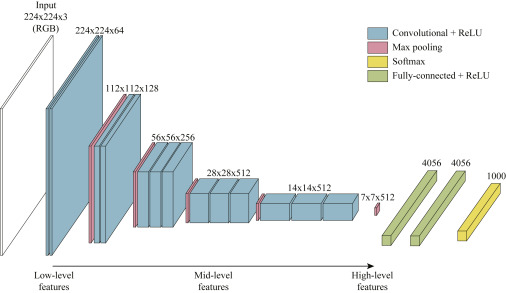
\includegraphics[width=10cm, height=5.5cm]{images/cnn.jpg}
    \caption{Przykładowa architektura konwolucyjnej sieci neuronowej\cite{artCnn}}
    \label{fig:cnn-architecture}
\end{figure}
\par
W celu dobrania odpowiedniej architektury sieci neuronowej do problemu oraz pewności wykorzystywania najbardziej nowoczesnych technik, warto śledzić wyniki międzynarodowych zawodów w dziedzinie rozpoznawania obrazów. Takim konkursem jest ImageNet Large Scale Visual Recognition Challenge (ILSVRC), odbywający się w latach 2010-2017, podczas którego zaprezentowanych zostało kilka architektur uważanych obecnie za \textit{state of the art}. 
\vspace{5mm}
\par
Wybrane architektury konwolucyjnych sieci neuronowych, odnoszące sukcesy w ImageNet ILSVRC challenge:
\begin{enumerate}
    \item AlexNet - zwycięzca z 2012 roku, dzięki któremu konwolucyjne sieci neuronowe zaczęły cieszyć się większą popularnością. Sieć ma 8 warstw, w tym 5 warstw konwolucyjnych, z czego 3 umieszczone są bezpośrednio jedna za drugą, co w momencie powstania sieci było raczej nowatorskim podejściem.
    \item VGG - sieć istniejąca w wariantach VGG16 oraz VGG19 (w zależności od liczby warstw), prezentująca podejście wykorzystujące większą liczbę mniejszych konwolucyjnych filtrów zamiast dużych warstw konwolucyjnych, prowadzące do redukcji liczby parametrów, ważnej w kontekście sieci głębokich. Wadą sieci VGG jest ogromna liczba parametrów oraz ilość używanej pamięci.
    \item GoogLeNet (Inception) - 22-warstwowa sieć wykorzystująca specjalne \textit{inception modules}, składające się ze zrównoleglonych warstw konwolucyjnych. Część z nich poprzedzona jest filtrami konwolucyjnymi o rozmiarach 1x1, pozwalającymi na zmniejszenie głębokości obrazu, a co za tym idzie liczby wykonywanych operacji. Wykorzystanie \textit{inception modules} pozwoliło również na znaczne zmniejszenie liczby parametrów.
        \begin{figure}[ht]
        \centering
        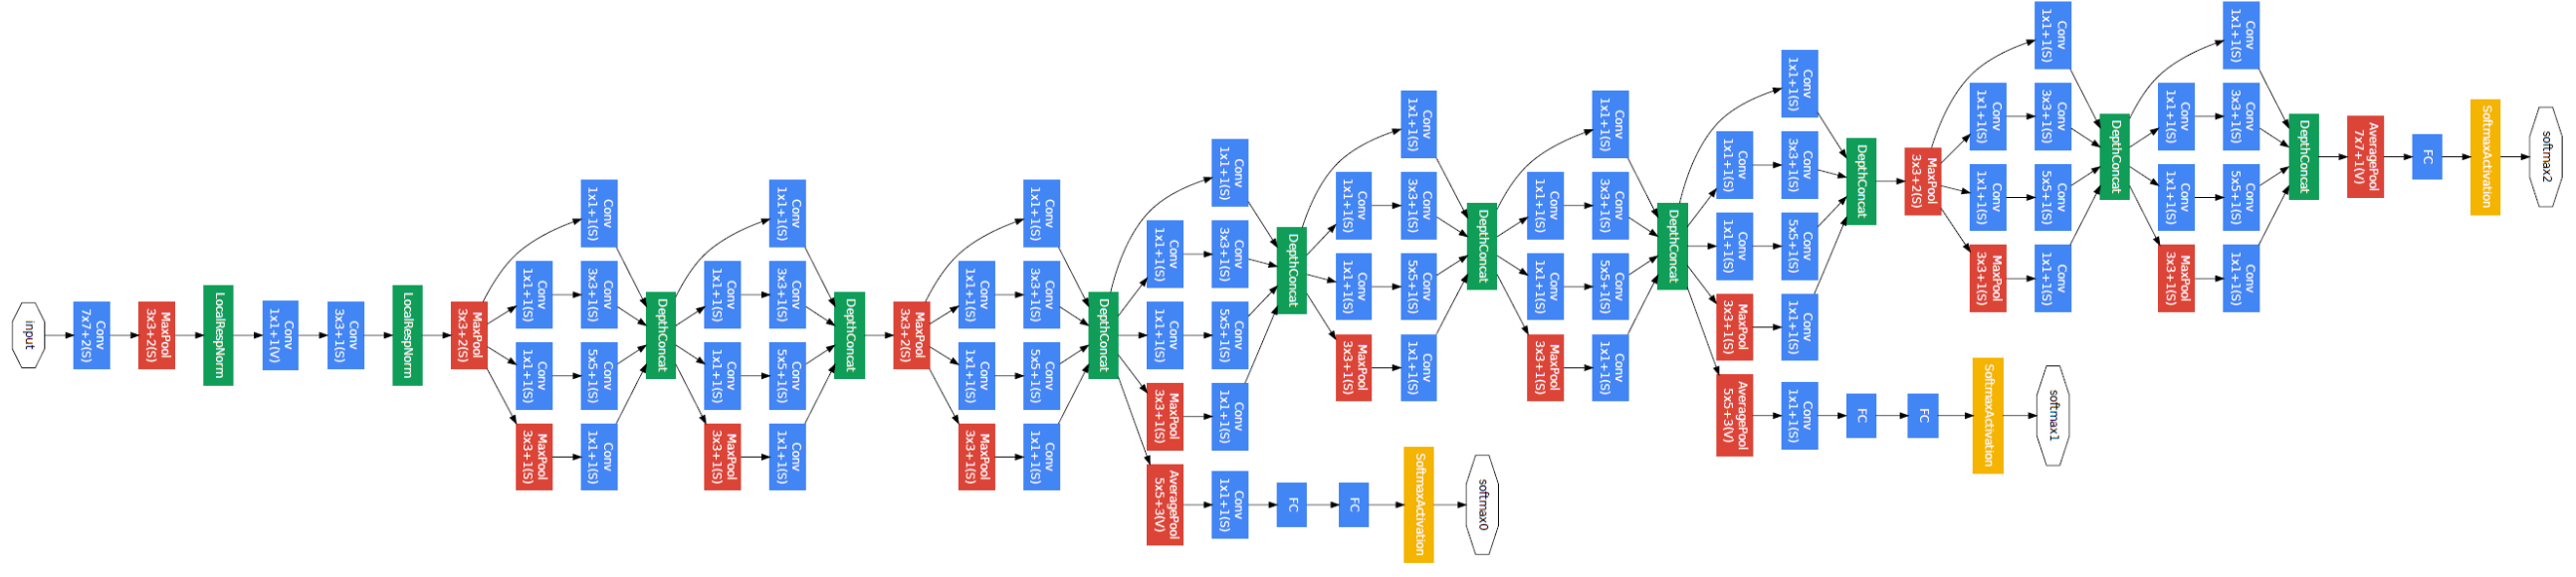
\includegraphics[width=16cm]{images/inception.png}
        \caption{Architektura sieci GoogLeNet\cite{artSzegedy}}
        \end{figure}
        \begin{figure}[ht]
        \centering
        \label{fig:googlenet-architecture}
        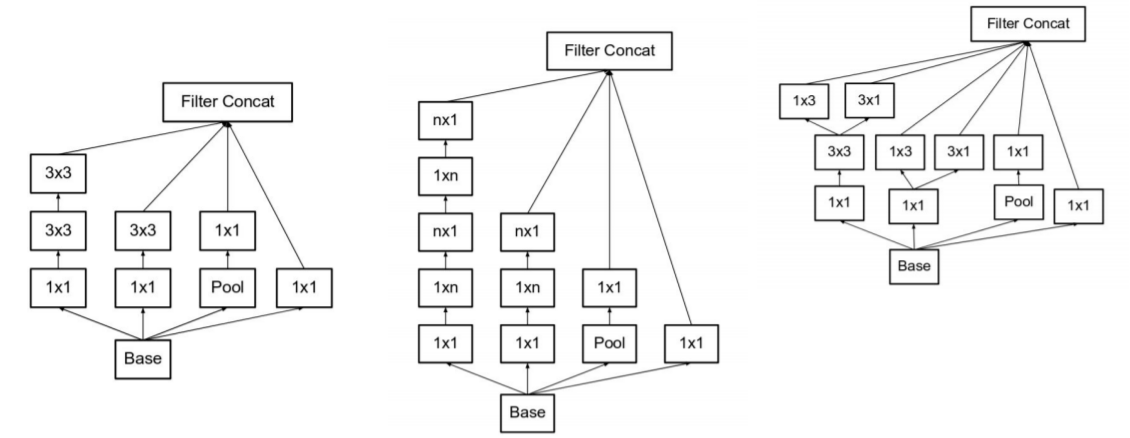
\includegraphics[width=15cm]{images/inception_module.PNG}
        \caption{Budowa pojedynczego \textit{inception module} w bardziej zaawansowanych wersjach\cite{artSzegedyRet}}
        \label{fig:inception-module}
        \end{figure}
    \item ResNet - głęboka (nawet 152 warstwy)  sieć, wykorzystująca połączenia rezydualne, które pozwalają na obliczenie zmiany na wyjściu w stosunku do parametrów wejściowych, poprzez włączenie do funkcji wyjściowej parametrów wejściowych z wagą 1. Sieć silnie wykorzystuje \textit{batch normalization} oraz nie posiada warstw \textit{fully connected} na końcu.
        \begin{figure}[ht]
        \centering
        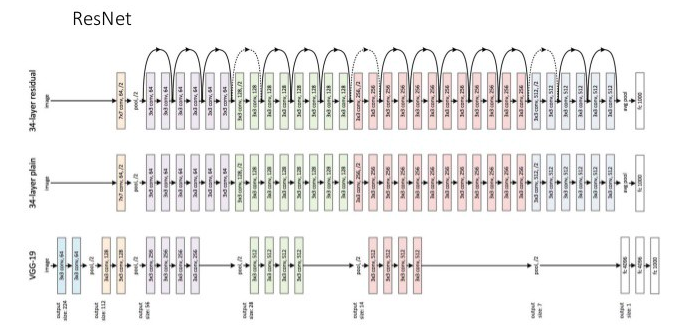
\includegraphics[width=16cm]{images/resnet.png}
        \caption{Architektura sieci ResNet\cite{artresnet}}
        \end{figure}
        \begin{figure}[ht]
        \centering
        \label{fig:resnet-architecture}
        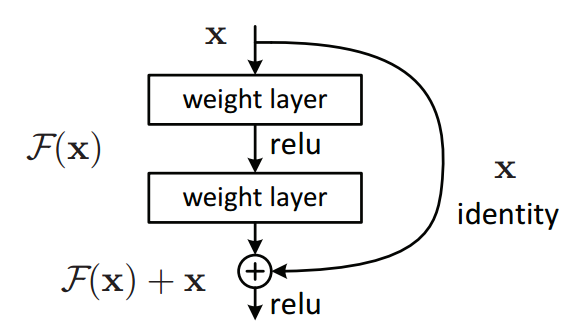
\includegraphics[width=6cm]{images/residual_block.png}
        \caption{Budowa rezydualnego połączenia\cite{artresnet}}
        \label{fig:res-block}
        \end{figure}
    \item ResNeXt - sieć będąca ulepszeniem ResNet, wprowadzająca równoległe bloki warstw konwolucyjnych w połączeniach rezydualnych.
    \item DenseNet - bardzo głęboka sieć posiadająca specjalne bloki (\textit{dense blocks}), w obrębie których każda warstwa połączona jest z wszystkimi warstwami, które znajdują się po niej.
\end{enumerate}

\par Inną architekturą, którą warto wziąć pod uwagę, jest architektura EfficientNet (dostępna z poziomu frameworka Keras). Powstała ona w 2019 roku i dzięki umiejętnemu skalowaniu głębokości i szerokości sieci oraz rozdzielczości zdjęć na wejściu, pozwoliła na uzyskanie lepszych wyników na zbiorze ImageNet w porównaniu do sieci ResNet, przy znacznym zmniejszeniu liczby parametrów i koniecznej do wykorzystania mocy obliczeniowej. Sieć posiada 8 wariantów (B0-B7), w których wraz z rosnącym numerem rośnie liczba parametrów.
\par
Ze względu na ilość dostępnych danych w momencie tworzenia modeli (kilkanaście tysięcy zdjęć), wykluczające wykorzystanie bardzo głębokich sieci, możliwość wykorzystania nowoczesnych architektur oraz kwestię dostępności tych architektur w Keras, spośród powyższych architektur w pracy zbadana zostanie jakość klasyfikacji dokonywana przez sieci ResNet, Inception oraz EfficientNet.

\subsection{Przegląd frameworków do tworzenia aplikacji webowych w języku Python}
\par Porównane zostaną dwa najbardziej popularne frameworki - Flask i Django. Ze względu na dobre wsparcie dla tworzenia aplikacji webowych w języku Python oferowane przez powyższe frameworki, a także łatwość integracji z nimi sieci trenowanej z wykorzystaniem innego frameworka języka Python, inne języki programowania nie będą brane pod uwagę.
\vspace{5mm}
\newline Flask:
\begin{enumerate}
    \item Mikro-framework dostarczający podstawowych funkcjonalności aplikacji webowej
    \item Łatwo można go poszerzać o dostępne w Pythonie biblioteki i dodatki
    \item Funkcjonalności frameworka są ograniczone i dodatkowe funkcjonalności muszą zostać dodane przy użyciu innych technologii
    \item Bardziej elastyczny niż Django - dobry dla aplikacji, w których w trakcie rozwoju będą podejmowane decyzje technologiczne
    \item Dobry do eksperymentowania z architekturą i bibliotekami, dla aplikacji składających się z nieznanej liczby wysoko wyspecjalizowanych (mikro)serwisów, dla aplikacji z wieloma małymi funkcjonalnościami
    \item Mniejszy niż Django, dobry, gdy aplikacji potrzebne są jedynie podstawowe możliwości frameworka
    \item Prostszy niż Django - szybsze wytwarzanie mniejszych funkcjonalności
\end{enumerate}
Django:
\begin{enumerate}
    \item Dostarcza system szablonów, wbudowane ORM, panel administratora
    \item “Konwencja ponad konfiguracją” - trudniejsze modyfikacje i dostosowywanie, prostsze rozwój i konserwacja
    \item Skrojony dla większych projektów wymagających dużej liczby funkcjonalności - dla mniejszych projektów może być zbyt rozbudowany
    \item Dostarcza ustandaryzowany i uproszczony proces tworzenia
    \item Szybsze niż we Flasku dopinanie frontendu - łatwiejsze tworzenie prototypów
    \item Większa społeczność używająca Django niż Flaska
\end{enumerate}
\par
Ze względu na charakterystykę tworzonej aplikacji - prostotę, dla której wystarczą podstawowe funkcjonalności aplikacji webowej, konieczność integracji aplikacji z frameworkiem TensorFlow, a także chęć pozostawienia przestrzeni na podjęcie niektórych ostatecznych decyzji technologicznych w późniejszych etapach pracy (ze względu na trudność przewidzenia jak dobrze zostanie wytrenowana sieć i przez to jaki zestaw funkcjonalności będzie ostatecznie udostępniony użytkownikowi), lepszym wyborem dla powstającego produktu jest framework Flask.

\newpage
\section{\SectionTitleScope}
\label{sec:zakres-funkcjonalnosci}
\par W poniższym rozdziale prezentowane są szczegółowe wymagania dla produktu, stanowiące podsumowanie etapu planowania. Rozdział umożliwia zapoznanie się z planowanymi użytkownikami oraz funkcjami systemu.

\subsection{Użytkownicy systemu}
\begin{enumerate}
    \item Użytkownik aplikacji webowej
    \newline Użytkowników aplikacji webowej podzielić można na dwie podkategorie:
    \begin{itemize}[noitemsep,topsep=0pt]
        \item Specjalista w dziedzinie poszyć samolotów
        \newline Główną grupą użytkowników, którym dedykowany jest powstający produkt, są specjaliści - posiadacze zdjęć z systemu DAIS, chcący szybko i skutecznie uzyskać odpowiedź na pytanie, czy na danym fragmencie poszycia znaleźć można oznaki korozji. Takich użytkowników interesować będą również wartości neuronów ostatniej warstwy sieci, odpowiedzialnych za predykcję, określające z jak dużym prawdopodobieństwem sieć przypisała zdjęciu dany wynik. Dodatkową, wartościową informacją są dla specjalistów informacje dotyczące fragmentów zdjęć głównie odpowiedzialnych za otrzymany wynik, mogące pomóc w lokalizacji rdzawych elementów. Dla tych użytkowników znaczenie mają głównie jakość oraz szybkość predykcji.
        \item Osoba zainteresowana tematyką lotniczą
        \newline Drugą grupą użytkowników, konieczną do wyszczególnienia, są osoby w mniejszym lub większym stopniu zainteresowane tematyką lotniczą, które weszły w posiadanie zdjęć poszycia samolotów (być może niepochodzących z systemu DAIS), chcące przetestować klasyfikator korozji. Dla takich użytkowników elementem zachęcającym do skorzystania z systemu będą estetyczny wygląd aplikacji oraz możliwość edycji zdjęcia poprzez zastosowanie filtrów i sprawdzenie jaki ma ona wpływ na otrzymany wynik. Ta grupa użytkowników traktuje system informacyjnie, w ramach ciekawostki, a sama jakość klasyfikacji nie ma dla nich dużego znaczenia.
    \end{itemize}
    \item Administrator systemu
    \newline Drugim rodzajem użytkowników systemu jest administrator, będący ekspertem dziedzinowym z dużą wiedzą matematyczno-informatyczną. Jego zadaniem jest aktualizacja używanego w aplikacji modelu sieci neuronowej oraz archiwizacja używanych wcześniej modeli. Administrator powinien dbać również o usuwanie zbędnych danych pochodzących od użytkowników, mogących pozostać w systemie w wyniku nieoczekiwanej przerwy w działaniu serwera, skutkującej brakiem ich usunięcia przez serwer.
\end{enumerate}

\newpage
\subsection{Przypadki użycia}
Do zaplanowania działania systemu oraz tego, jak użytkownik będzie korzystał z jego funkcji, wykorzystane zostały przypadki użycia. Z diagramu oraz opisów łatwo wywnioskować sposób interakcji użytkowników z systemem, możliwości poszczególnych aktorów oraz wewnętrzne zasady działania aplikacji, dzięki czemu można szybko zlokalizować braki czy problemy zaproponowanego układu. 

\begin{figure}[h]
    \centering
    \label{fig:use-case-diagram}    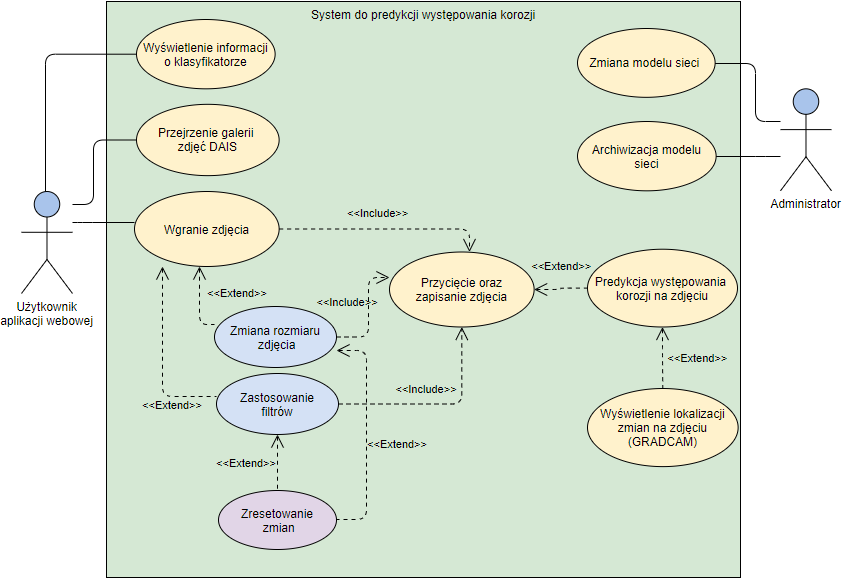
\includegraphics[width=16cm]{images/usecase-diagram-admin.PNG}
    \caption{Diagram przypadków użycia}
\end{figure}

Poniżej opisane zostały wybrane przypadki użycia. W bardziej złożonych przypadkach przedstawiono scenariusz główny oraz alternatywny. Nie wszystkie przypadki zostały zamieszczone ze względu na oczywisty przebieg interakcji między aktorem a systemem w niektórych sytuacjach.

\begin{table}[h!]
\centering
 \begin{tabular}{|m{4cm}|m{11cm}|} 
 \hline
 Tytuł & Wyświetlenie informacji o klasyfikatorze\\
 \hline
 Aktor główny & Użytkownik aplikacji webowej\\
 \hline
 Cel & Uzyskanie informacji o klasyfikatorze\\ 
 \hline
 Kontekst użycia & Użytkownik systemu chce uzyskać informacje na temat klasyfikatora, który jest używany przez aplikację\\ 
 \hline
 Warunek początkowy & Użytkownik uruchomił aplikację webową\\
 \hline
 Zdarzenie inicjujące & Użytkownik naciska przycisk prowadzący do informacji o klasyfikatorze\\
 \hline
\end{tabular}
\caption{Przypadek użycia: Wyświetlenie informacji o klasyfikatorze}
\label{table:1}
\end{table}

\newpage
\begin{table}[h!]
\centering
 \begin{tabular}{|m{4cm}|m{11cm}|} 
 \hline
 Tytuł & Przejrzenie galerii zdjęć DAIS\\
 \hline
 Aktor główny & Użytkownik aplikacji webowej\\
 \hline
 Cel & Obejrzenie zdjęć wykonanych w ramach systemu DAIS\\ 
 \hline
 Kontekst użycia & Użytkownik systemu chce zobaczyć, na jakich zdjęciach można dokonać predykcji\\ 
 \hline
 Warunek początkowy & Użytkownik uruchomił aplikację webową\\
 \hline
 Zdarzenie inicjujące & Użytkownik uruchamia aplikację webową\\
 \hline
\end{tabular}
\caption{Przypadek użycia: Przejrzenie galerii zdjęć DAIS}
\label{table:2}
\end{table}

\begin{table}[h!]
\centering
 \begin{tabular}{|m{4cm}|m{11cm}|} 
 \hline
 Tytuł & Wgranie zdjęcia\\
 \hline
 Aktor główny & Użytkownik aplikacji webowej\\
 \hline
 Cel & Załadowanie zdjęcia z dysku do aplikacji\\ 
 \hline
 Kontekst użycia & Użytkownik systemu chce uzyskać informacje na temat występowania korozji na obiekcie przedstawionym na zdjęciu, przechowywanym na dysku swojego komputera\\ 
 \hline
 Warunek początkowy & Użytkownik uruchomił aplikację webową oraz posiada zdjęcie obiektu do predykcji\\
 \hline
 Zdarzenie inicjujące & Użytkownik naciska przycisk służący do wgrania zdjęcia\\
 \hline
\end{tabular}
\caption{Przypadek użycia: Wgranie zdjęcia}
\label{table:3}
\end{table}

\noindent
Główny scenariusz powodzenia:
\begin{enumerate}
    \item System wyświetla pole do wgrania zdjęcia
    \item Użytkownik wybiera zdjęcie z dysku w jednym z formatów: jpg, jpeg, png, bmp
    \item System wyświetla okno do dalszej edycji wgranego zdjęcia
\end{enumerate}
Scenariusz alternatywny:
\begin{itemize}
    \item Format pliku wgranego przez użytkownika jest inny niż obsługiwane przez aplikację $\,\to\,$ System zamyka pole do wyboru zdjęcia
\end{itemize}

\begin{table}[h!]
\centering
 \begin{tabular}{|m{4cm}|m{11cm}|} 
 \hline
 Tytuł & Zastosowanie filtrów\\
 \hline
 Aktor główny & Użytkownik aplikacji webowej\\
 \hline
 Cel & Zastosowanie filtrów na wgranym zdjęciu\\ 
 \hline
 Kontekst użycia & Użytkownik systemu chce zmodyfikować oryginalne zdjęcie stosując filtry\\ 
 \hline
 Warunek początkowy & Użytkownik wgrał zdjęcie w odpowiednim formacie\\
 \hline
 Zdarzenie inicjujące & Użytkownik naciska przycisk przy nazwie filtra, który chce zastosować\\
 \hline
\end{tabular}
\caption{Przypadek użycia: Zastosowanie filtrów}
\label{table:4}
\end{table}

\noindent
Główny scenariusz powodzenia:
\begin{enumerate}
    \item Użytkownik zaznacza filtr, który chce zastosować
    \item System sprawdza, jakie filtry są zaznaczone i wyświetla obraz z zastosowanymi filtrami
\end{enumerate}

\FloatBarrier\clearpage
\begin{table}[h!]
\centering
 \begin{tabular}{|m{4cm}|m{11cm}|} 
 \hline
 Tytuł & Predykcja występowania korozji na zdjęciu\\
 \hline
 Aktor główny & Użytkownik aplikacji webowej\\
 \hline
 Cel & Uzyskanie predykcji dot. występowania korozji na wgranym z dysku zdjęciu\\ 
 \hline
 Kontekst użycia & Użytkownik systemu chce uzyskać informacje na temat występowania korozji na obiekcie przedstawionym na przetworzonym zdjęciu\\ 
 \hline
 Warunek początkowy & Użytkownik przyciął i zapisał wgrane zdjęcie\\
 \hline
 Zdarzenie inicjujące & Użytkownik naciska przycisk służący do predykcji\\
 \hline
\end{tabular}
\caption{Przypadek użycia: Predykcja występowania korozji na zdjęciu}
\label{table:5}
\end{table}

\noindent
Główny scenariusz powodzenia:
\begin{enumerate}
    \item Użytkownik naciska przycisk do predykcji
    \item System wyświetla wyniki predykcji występowania korozji uzyskane za pomocą modelu sieci: etykietę prawdziwej klasy, etykietę przewidzianej klasy oraz stopień przynależności do klasy korozji i klasy braku korozji
\end{enumerate}
Scenariusz alternatywny:
\begin{itemize}
    \item Nazwa zdjęcia nie zawiera informacji o prawdziwej klasie obiektu $\,\to\,$ System nie wyświetla informacji o prawdziwej klasie obiektu
\end{itemize}

\begin{table}[h!]
\centering
 \begin{tabular}{|m{4cm}|m{11cm}|} 
 \hline
 Tytuł & Zmiana modelu sieci\\
 \hline
 Aktor główny & Administrator\\
 \hline
 Cel & Zmiana modelu sieci używanego do predykcji występowania korozji\\ 
 \hline
 Kontekst użycia & Administrator chce wprowadzić do aplikacji inny model sieci neuronowej\\ 
 \hline
 Warunek początkowy & Uwierzytelnienie administratora zakończone sukcesem oraz posiadanie przez administratora na dysku modelu, który chce wgrać do aplikacji\\
 \hline
 Zdarzenie inicjujące & Administrator wybrał przycisk do zmiany modelu\\
 \hline
\end{tabular}
\caption{Przypadek użycia: Zmiana modelu sieci}
\label{table:6}
\end{table}

\noindent
Główny scenariusz powodzenia:
\begin{enumerate}
    \item System wyświetla pole do wgrania modelu
    \item Administrator wybiera model sieci z dysku
    \item System aktualizuje model wykorzystywany do predykcji
\end{enumerate}

\newpage
\subsection{Ustalony zakres prac}
\par Ustalony zakres prac obejmuje realizację następujących wymagań funkcjonalnych i niefunkcjonalnych:
\vspace{5mm}
\par\noindent Wymagania funkcjonalne:
\begin{enumerate}
    \item Wgranie zdjęcia
    \item Możliwość aplikacji różnych filtrów dla wgrywanego zdjęcia: szumu gaussowskiego, transformaty Fouriera, konturowania, wyostrzenia, transformacji do skali szarości
    \item Możliwość zmiany rozmiaru wgrywanego zdjęcia
    \item Prezentacja wyników predykcji wraz z podaniem konkretnych wartości neuronów wyjściowych dla każdej klasy oraz (jeśli została podana) oryginalnej etykiety zdjęcia
    \item Prezentacja pikseli głównie odpowiedzialnych za wynik predykcji w postaci heatmapy
\end{enumerate}

\noindent
Wymagania niefunkcjonalne:
\begin{enumerate}
    \item Akceptowanie przez system zdjęć w dowolnym spośród najpopularniejszych formatów przeznaczonych dla obrazów: jpg, jpeg, png, bmp
    \item Możliwość jednoczesnego korzystania z systemu przez wielu użytkowników
    \item Interfejs dostosowany do użytku przez użytkowników niemających wcześniej styczności z tematyką sieci neuronowych i klasyfikacji przez nie zdjęć
    \item Realizacja systemu w formie aplikacji webowej
    \item Nieprzechowywanie przesyłanych przez użytkowników zdjęć po zakończeniu interakcji użytkownika z systemem
\end{enumerate}

\vspace{5mm}
\par Przewiduje się, że (przynajmniej na początku swojego działania) system nie będzie wymagał obsługi bardzo dużej liczby jednoczesnych użytkowników, a także zakłada się brak konieczności dodatkowego zabezpieczania przesyłanych przez nich zdjęć. Dodatkowo ustalono, że nie będzie tworzona osobna część systemu przewidziana dla administratora, zaś przewidziane funkcjonalności podmiany modelu sieci i archiwizacji modeli oraz usuwania niepotrzebnych danych pochodzących od użytkowników będą realizowane na poziomie kodu źródłowego i systemu plików.

\newpage
\subsection{Opis procesów biznesowych}

\par\noindent Wyszczególniono następujące procesy biznesowe:
\vspace{5mm}
\newline Proces przygotowania zdjęcia:

\begin{figure}[h]
    \centering
    \label{fig:prepare-image-proccess}    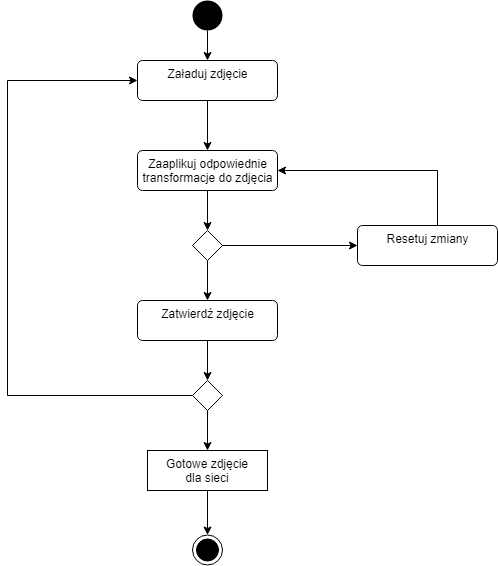
\includegraphics[width=12cm]{images/proces_przygotowania.png}
    \caption{Diagram aktywności dla procesu przygotowania zdjęcia}
\end{figure}

\par W typowym przebiegu procesu przygotowania zdjęcia użytkownik załadowuje zdjęcie, aplikuje do niego odpowiednie transformacje i zatwierdza zdjęcie, w wyniku czego powstaje obraz gotowy do wykorzystania przez sieć neuronową. Proces ten przewiduje jednak również w swoim przebiegu możliwość wystąpienia pewnych odstępstw. Po aplikacji transformacji użytkownik może je wycofać, resetując zdjęcie do początkowej postaci, a następnie zaaplikować transformacje ponownie i postępować dalej zgodnie z możliwym przebiegiem procesu. Drugim odstępstwem od typowego przygotowania zdjęcia jest decyzja o ponownym załadowaniu zdjęcia (tego samego lub innego) po wykonaniu kroków związanych z aplikacją transformacji i zatwierdzeniu obrazu. Przewiduje się, że powyższe alternatywne przebiegi omawianego procesu będą występowały znacznie rzadziej niż przebieg uznany za typowy.

\newpage

Proces zbierania wyników:

\begin{figure}[h]
    \centering
    \label{fig:predict-proccess}    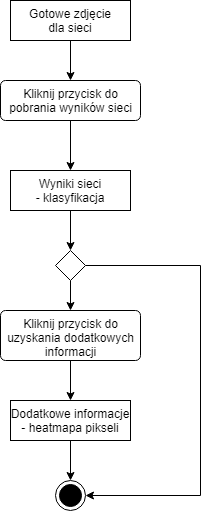
\includegraphics[width=5.5cm]{images/proces_zbierania_wynikow.png}
    \caption{Diagram aktywności dla procesu zbierania wyników}
\end{figure}

\par Punktem wyjścia dla procesu zbierania wyników jest obraz powstały w procesie przygotowania zdjęcia. W omawianym procesie użytkownik otrzymuje wyniki sieci dotyczące klasyfikacji zdjęcia po kliknięciu odpowiedniego przycisku do ich pobrania. W typowym przebiegu procesu kolejnym wykonywanym przez użytkownika krokiem jest kliknięcie przycisku do uzyskania dodatkowych informacji, skutkujące wyświetleniem heatmapy ukazującej piksele głównie odpowiadające za wynik klasyfikacji oraz tej samej heatmapy nałożonej na oryginalne zdjęcie. Krok ten może jednak zostać pominięty - wtedy proces pobierania wyników kończy się uzyskaniem wyniku klasyfikacji (przewiduje się jednak, że jest to ścieżka, która wystąpi rzadziej niż ta uznana za typową).

\newpage
\section{\SectionTitleRealizationAspects}
\label{sec:wybrane-aspekty-realizacji}
\par Rozdział zawiera informacje dotyczące sposobu realizacji stworzonego systemu, a więc zarówno dane dotyczące aplikacji webowej, jak i drogę przebytą w celu uzyskania sieci neuronowej, możliwej do wykorzystania w końcowym produkcie. Zawarte w tym rozdziale informacje mogą być przydatne dla osób chcących dalej rozwijać produkt.

\subsection{Ogólny rzut na sposób działania systemu}
W systemie zdarzenia są inicjowane przez użytkownika aplikacji, który wykonuje działania w przeglądarce internetowej. Przeglądarka, jako klient, wysyła zapytania HTTP do serwera, którego funkcję pełni aplikacja, zbudowana w oparciu o framework Flask. 

\begin{figure}[h]
    \centering
    \label{fig:sequence-diagram}    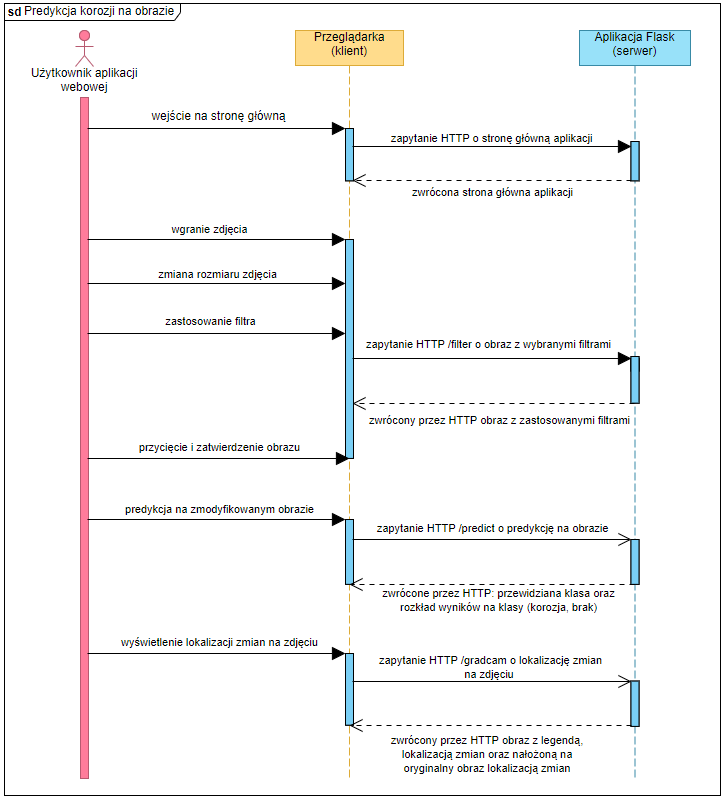
\includegraphics[width=15cm]{images/diagram_sekwencji.PNG}
    \caption{Diagram sekwencji}
\end{figure}

Aplikacja to HTTP API z serwerem działającym na zasadzie RPC - klient wysyła zapytanie z potrzebnymi do wywołania procedury argumentami, a w odpowiedzi uzyskuje wynik wywołania procedury na serwerze (zdjęcie, tekst do wyświetlenia). Strona klienta odpowiedzialna jest za odpowiednie wyświetlenie dostarczonych przez protokół danych. Zgodnie z założeniami protokołu HTTP o bezstanowości, żadne dane z zapytań nie są przechowywane przez serwer i za każdym razem przesyłane są wszystkie potrzebne do zrealizowania żądania informacje (m.in. zdjęcie, na którym przeprowadzana jest predykcja). W przypadku strony głównej oraz filtrów wysyłane są zapytania synchroniczne. Użytkownik, wybierając różne filtry oczekuje, że otrzyma wyniki w takiej kolejności, w jakiej zostały wybierane. Asynchronicznie wysyłane są zapytania o predykcję występowania korozji oraz lokalizację zmian na zdjęciu. Niektóre z działań użytkownika nie wymagają uzyskania informacji od serwera, np. zmiana rozmiaru zdjęcia.

\subsection{Struktura systemu}
\par W tym podrozdziale zawarte zostały informacje dotyczące implementacji systemu - struktura kodu źródłowego oraz opisy części serwerowej i klienckiej powstałej aplikacji. Przedstawiono aspekty szczególnie przydatne osobom chcącym dalej rozwijać projekt na poziomie aplikacji webowej.

\subsubsection{Struktura kodu źródłowego}
\par Na poniższym rysunku przedstawiona została struktura kodu źródłowego aplikacji:

\begin{figure}[h!]
    \centering
    \label{fig:source-code-structure}    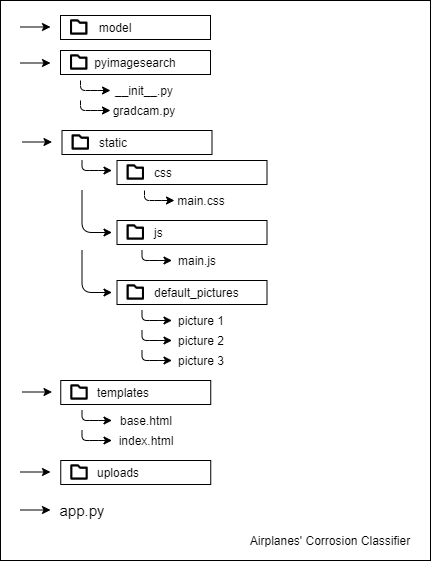
\includegraphics[width=8.6cm]{images/struktura_systemu.png}
    \caption{Struktura kodu źródłowego stworzonego projektu}
\end{figure}

\par\noindent Opis poszczególnych elementów:
\begin{itemize}
    \item model: katalog zawierający zapisany model sieci (struktura, wagi), wykorzystywany podczas predykcji oraz do tworzenia heatmapy pikseli
    \item pyimagesearch: pakiet zawierający implementację fragmentu aplikacji odpowiedzialnego za tworzenie heatmapy pikseli głównie odpowiedzialnych za predykcję
    \item static: katalog zawierający elementy statyczne aplikacji webowej, tzn. kod css i javascript, a także zdjęcia z galerii DAIS
    \item templates: katalog zawierający kod html strony
    \item uploads: katalog do chwilowego przechowywania zdjęć użytkownika i tworzonych w odpowiedzi dla klienta obrazów
    \item app.py: plik w języku Python, zawierający logikę serwerowej części aplikacji
\end{itemize}

\subsubsection{Serwer i klient}
\par Serwer:
\newline Część serwerowa aplikacji udostępnia szereg usług, dostępnych poprzez zapytania HTTP:
\renewcommand{\arraystretch}{1.75}
\begin{table}[h!]
\centering
 \begin{tabular}{|m{5cm}|m{3.5cm}|m{3.7cm}|m{2cm}|} 
 \hline
 Usługa & Nazwa funkcji & Nazwa metody HTTP & URI\\
 \hline
 Wyświetlenie strony & index & GET & /\\
 \hline
 Przesłanie zdjęcia do predykcji i zwrócenie wyników & upload & GET, POST & /predict\\
 \hline
 Aplikacja filtra do zadanego zdjęcia i zwrócenie wyników & filters & GET, POST & /filter\\
 \hline
 Przygotowanie heatmapy dla spredykowanego zdjęcia i zwrócenie wyników & gradcam\_info & GET, POST & /gradcam\\
 \hline
\end{tabular}
\caption{Opis udostępnianych przez serwer usług}
\label{table:7}
\end{table}

\par\noindent Dodatkowe informacje o zaimplementowanych w części serwerowej funkcjach:
\begin{itemize}
    \item upload: 
    \begin{itemize}
        \item pobranie obrazu z żądania HTTP
        \item zapisanie obrazu na czas dokonywanej predykcji - nazwa pliku generowana z UUID
        \item jeśli nazwa obrazu zawiera informację dotyczącą poprawnej etykiety obrazu - pobranie tej etykiety
        \item przeprowadzenie odpowiedniego dla sieci neuronowej preprocessingu obrazu
        \item przeprowadzenie predykcji na modelu
        \item usunięcie obrazu z systemu plików
        \item przygotowanie odpowiedzi
        \item zwrócenie przygotowanej odpowiedzi w formacie JSON
    \end{itemize}
    \item filters:
    \begin{itemize}
        \item pobranie obrazu z żądania HTTP
        \item zapisanie obrazu na czas dokonywanej transformacji - nazwa pliku generowana z UUID
        \item pobranie z żądania HTTP rodzajów filtrów z informacją, czy mają zostać zastosowane. Dla podstawowych filtrów jest to określone binarnie. W przypadku rozmycia Gaussowskiego i transformaty Fouriera otrzymywana jest sigma - liczba naturalna. 
        \item zastosowanie po kolei filtrów z nadpisaniem oryginalnego obrazu w systemie plików obrazem wynikowym
        \item przygotowanie odpowiedzi - kodowanie obrazu do base64
        \item usunięcie obrazu z systemu plików
        \item zwrócenie przygotowanej odpowiedzi 
    \end{itemize}
    \item gradcam\_info:
    \begin{itemize}
        \item pobranie obrazu z żądania HTTP
        \item zapisanie obrazu na czas tworzenia heatmapy - nazwa pliku generowana z UUID
        \item przygotowanie wyjściowego obrazu z nadpisaniem oryginalnego obrazu w systemie plików obrazem wynikowym
        \item przygotowanie odpowiedzi - kodowanie do base64
        \item usunięcie obrazu z systemu plików
        \item zwrócenie przygotowanej odpowiedzi 
    \end{itemize}
\end{itemize}

\par\noindent Klient:
\par Klientem w wytworzonym systemie jest przeglądarka internetowa, za pośrednictwem której użytkownik dokonuje interakcji z serwerem. Klient zbiera dane od użytkownika. We wszystkich zapytaniach przesyłany jest obraz, natomiast w zapytaniach o zastosowanie filtra wysyłane są nazwy wszystkich filtrów z informacją, czy należy je nałożyć na obraz (w przypadku filtrów skali szarości, wyostrzania oraz uzyskania konturów informacja przekazywana jest binarnie, zaś poziomy transformaty Fouriera i rozmycia gaussowskiego opisane są liczbami naturalnymi). W kolejnym kroku klient konstruuje formularz, do którego wprowadza dane (obrazy wprowadzane są w postaci BLOB), a następnie przesyła je serwerowi przy pomocy zapytań HTTP. Serwer odsyła klientowi odpowiedź, którą klient wyświetla na ekranie w przyjaznej użytkownikowi formie.
\par Część kliencka aplikacji napisana została przy użyciu HTML, CSS i JavaScript (interakcja użytkownika z aplikacją możliwa jest dzięki kodowi javascriptowemu).
\par W celu skrócenia i ułatwienia procesu tworzenia kodu w JavaScripcie, podczas tworzenia aplikacji wykorzystano bibliotekę JQuery. Umożliwia ona uproszczone w stosunku do czystego JavaScriptu manipulacje kodem HTML i CSS, obsługę \textit{eventów}, tworzenie animacji oraz obsługę AJAX.
\par Zapytania dla serwera wysyłane są przy użyciu AJAX. Technika ta umożliwia pobieranie informacji z serwera i asynchroniczne wyświetlanie ich bez konieczności przeładowywania strony. Sposób działania AJAX można przedstawić w następujących punktach\cite{ajax}:
\begin{enumerate}
    \item Wystąpienie zdarzenia na stronie (kliknięty przycisk, załadowanie strony)
    \item Stworzenie obiektu XMLHttpRequest przez JavaScript
    \item Wysłanie zapytania do serwera przez XMLHttpRequest
    \item Przetworzenie zapytania przez serwer
    \item Przesłanie odpowiedzi od serwera do strony
    \item Przeczytanie odpowiedzi przez JavaScript
    \item Wykonanie odpowiedniej akcji przez JavaScript (np. aktualizacja strony)
\end{enumerate}
Zapytania do serwera takie jak zapytanie o wynik predykcji na zdjęciu oraz zapytanie o heatmapę pikseli wykonywane są asynchronicznie, natomiast zapytania dotyczące aplikacji filtrów do zdjęcia wykonywane są synchronicznie w celu zapewnienia użytkownikowi właściwej odpowiedzi.

\subsection{Droga poszukiwania sieci neuronowej dla systemu}

\par Najważniejszym elementem, wokół którego zbudowana jest aplikacja, jest wykorzystana sieć neuronowa. W tym podrozdziale pokazano drogę poszukiwania sieci użytecznej dla tworzonego systemu, a więc odznaczającej się nie tylko możliwie wysokim poziomem \textit{accuracy}, ale również jak najmniejszą liczbą przykładów fałszywie negatywnych.

\subsubsection{Superkomputer Prometheus}
\par Trenowanie sieci neuronowych jest procesem czasochłonnym, dodatkowo modele z dużą ilością parametrów wymagają odpowiednio dużej przestrzeni dyskowej. Sam proces uczenia najlepiej jest przeprowadzać na procesorach graficznych, umożliwiających silne zrównoleglenie tego procesu, pozwalające znacznie skrócić czas konieczny do wytrenowania sieci. Ze względu na przewidywaną dużą liczbę trenowanych modeli, wielkość ich architektur oraz rozmiar wykorzystywanych danych, koniecznym okazało się wykorzystanie maszyn udostępnianych przez organizacje zewnętrzne.
\par W projekcie wykorzystany został dostęp do Infrastruktury PLGrid, dokładniej do klastra Prometheus (326-te miejsce w rankingu superkomputerów Top 500 - stan na 11.2020) znajdującego się w Akademickim Centrum Komputerowym CYFRONET AGH w Krakowie. W celu wykorzystania jego zasobów konieczne było uzyskanie grantu obliczeniowego PLGrid oraz dostępu do klastra. 
\par Superkomputer Prometheus umożliwił dostęp do kart GPGPU, w tym kart Nvidia v100, co pozwoliło na skuteczne i możliwie wydajne przeprowadzenie treningów sieci neuronowych. W grancie wynegocjowane zostało również 1000GB przestrzeni dyskowej, co umożliwiało przeprowadzanie treningów bez konieczności przenoszenia wytrenowanych modeli na inne dyski w celu zwolnienia miejsca na nowe modele.
\par Zlecanie zadań na superkomputerze Prometheus odbywa się poprzez system kolejkowy SLURM. Do uruchomienia zadania konieczne było przygotowanie odpowiedniego skryptu. Dostęp do Prometheusa realizowany był poprzez łączenie się z maszyną dostępową za pomocą SSH, do czego wykorzystywany był program PuTTY.


\subsubsection{Zbiór danych}

\par\noindent Zbiór danych wykorzystany w pracy obejmował 13075 zdjęć poszycia statków powietrznych (o rozmiarach 640x480 pikseli), wykonanych w latach 2002-2020, pochodzących z 37 maszyn. Zdjęcia te zostały opisane przez specjalistów, którzy podzielili je na 5 klas:
\begin{itemize}
    \item brak korozji: 6431 zdjęć
    \item korozja lekka: 6040 zdjęć
    \item korozja średnia: 578 zdjęć
    \item korozja silna: 0 zdjęć
    \item niewielkie zniszczenia: 26 zdjęć
\end{itemize}
Ze względu na stosunkowo niedużą liczbę dostępnych zdjęć oraz niezrównoważenie liczby przykładów pomiędzy klasami, zdecydowano się podejść do problemu jako zadania binarnej klasyfikacji zdjęć dla klas: ``korozja'', ``brak korozji''.
\par Dla możliwie najlepszej symulacji wykorzystania sieci na nowych danych, podczas podziału zdjęć na zbiory: treningowy, walidacyjny i testowy zdecydowano się na utworzenie tych zbiorów ze zdjęć pochodzących z różnych maszyn. W ten sposób zbiór treningowy złożony był ze zdjęć maszyn 1-30 i obejmował 10343 zdjęcia (79\% zbioru danych), zbiór walidacyjny złożony był ze zdjęć maszyn 31-34 i zawierał 1448 zdjęć (11\% zbioru danych), zaś zbiór testowy zawierał zdjęcia pochodzące z maszyn 35-37, tj. 1284 zdjęcia (10\% zbioru). Podczas treningu, w celu zwiększenia zbioru treningowego, zastosowano augmentację danych polegającą na losowym przerzucaniu zdjęć względem osi X lub Y.
\par Ze względu na stosunkowo niewielką liczbę zdjęć oraz duży rozmiar pojedynczego zdjęcia, został stworzony drugi zbiór, posiadający zdjęcia o dwukrotnie zmniejszonej rozdzielczości (tj. 320x240 pikseli).

\subsubsection{Miary oceny klasyfikatora}
\par\noindent Jakość klasyfikacji oceniana była na podstawie poniższych metryk:
\begin{itemize}
    \item Accuracy (Acc) - liczba poprawnych predykcji podzielona przez liczbę wszystkich predykcji
    \item Loss - różnica między rzeczywistymi wartościami etykiet i prognozą dokonaną przez model
    \item True Positives (TP) - liczba poprawnie sklasyfikowanych przykładów dla klasy pozytywnej, w tym przypadku dla klasy ``korozja''
    \item False Positives (FP) - liczba niepoprawnie przydzielonych pozytywnych etykiet dla klasy negatywnej, w tym przypadku etykiet  ``korozja'' dla przykładów z klasy ``brak korozji''
    \item True Negatives (TN) - liczba poprawnie sklasyfikowanych przykładów dla klasy negatywnej, w tym przypadku dla klasy ``brak korozji''
    \item False Negatives (FN) - liczba niepoprawnie przydzielonych negatywnych etykiet dla klasy pozytywnej, w tym przypadku etykiet ``brak korozji'' dla przykładów z klasy ``korozja''
    \item Precision (Prec) - stosunek liczby przykładów poprawnie zaklasyfikowanych jako pozytywne do liczby wszystkich przykładów zaklasyfikowanych jako pozytywne (TP / (TP+FP))
    \item Recall (Rec) - stosunek liczby przykładów poprawnie zaklasyfikowanych jako pozytywne do liczby wszystkich przykładów rzeczywiście należących do klasy pozytywnej (TP / (TP+FN))
\end{itemize}

\subsubsection{Prosta architektura z warstwami konwolucyjnymi}

\par\noindent Początkowe podejście do problemu polegało na próbie wytrenowania sieci złożonej samodzielnie z warstw dostępnych we frameworku Keras. Zaproponowana architektura składała się z 5 bloków konwolucyjnych. Podstawą pojedynczego bloku były warstwy konwolucyjne z filtrem konwolucyjnym $3\times3$ i funkcją aktywacji ReLU. Do każdej takiej warstwy była dołączona warstwa normalizująca (Batch Normalization). W blokach znajdowały się jedna lub dwie tak złożone warstwy, a za nimi ustawiona była warstwa Max Pooling, redukująca rozmiar poprzednich warstw sieci. Po pięciu takich blokach, w celu otrzymania końcowego wyniku, dołożone zostały warstwy Global Average Pooling oraz Sigmoid.

\begin{figure}[h!]
    \centering
    \label{fig:simple-architecture-schema}    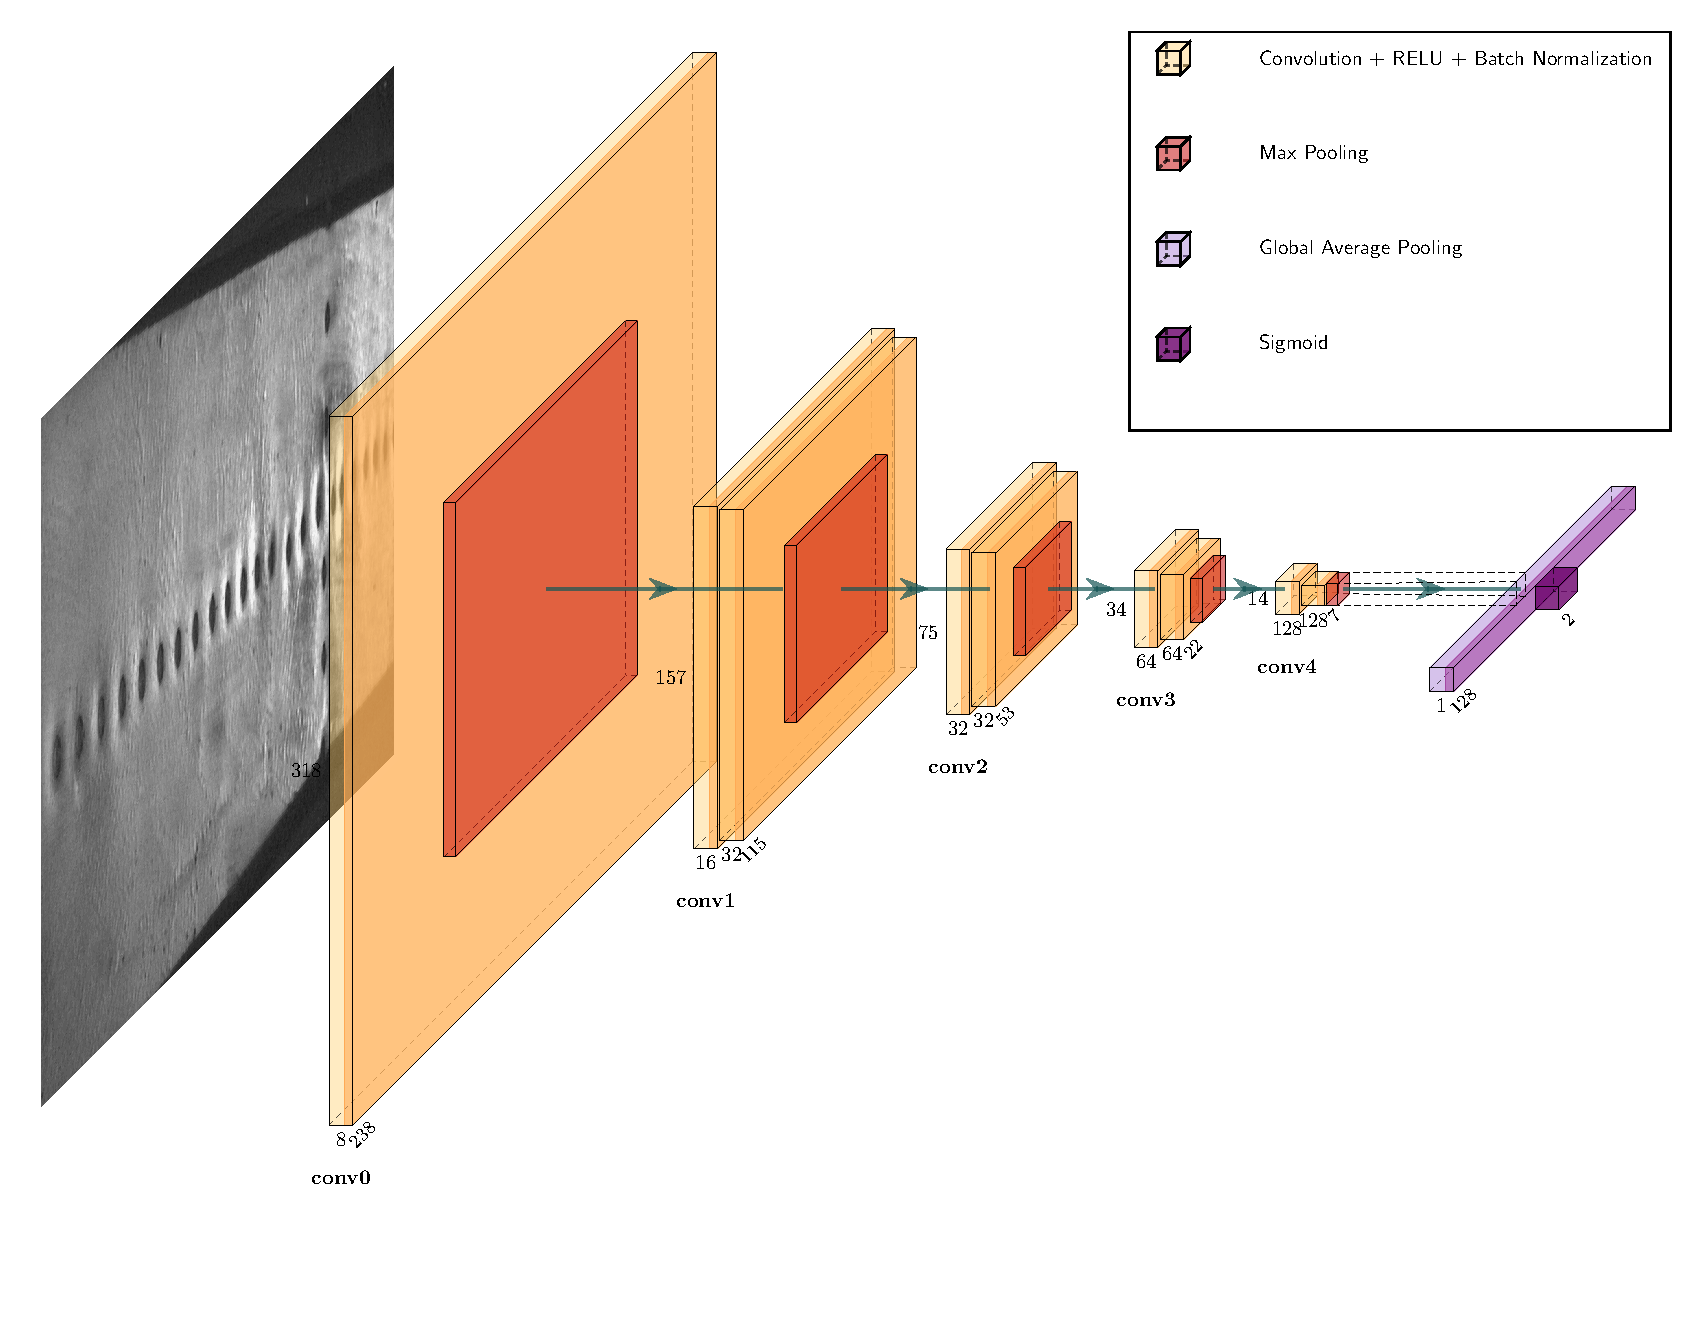
\includegraphics[width=16cm]{images/SimpleArchSchema.pdf}
    \caption{Schemat samodzielnie złożonej architektury}
\end{figure}

Tak zbudowana architektura była trenowana na zbiorze treningowym przez 20 epok. Biorąc pod uwagę małą liczbę warstw, uzyskane \textit{accuracy} wynoszące 76\% jest dobrym wynikiem. Wartość \textit{precision} wyniosła 84\%, jednak \textit{recall} wyniósł 69\%. Specyfika projektu wymaga minimalizacji wyników fałszywie negatywnych, ponieważ poważniejsze zagrożenie wynika ze złego przyporządkowania skorodowanego zdjęcia do klasy negatywnej niż na odwrót. Z tego powodu niski wynik \textit{recall} dla prostej sieci był niezadowalający. 


\begin{table}[h!]
\centering
 \begin{tabular}{|m{1.2cm}|m{1.2cm}|m{1.2cm}|m{1.2cm}|m{1.2cm}|m{1.2cm}|m{1.2cm}|m{1.2cm}|}
 \hline
 Acc & Loss & TP & FP & TN & FN & Prec & Rec\\
 \hline
 0.76 & 0.5 & 498 & 93 & 473 & 220 & 0.84 & 0.69\\
 \hline
 \end{tabular}
 \caption{Miary jakości sieci dla samodzielnie wykonanej architektury na zbiorze zdjęć o rozmiarze 320x240 pikseli}
 \label{table:8}
\end{table}

\begin{figure}[h!]%
    \begin{adjustbox}{minipage=1.0\paperwidth, pagecenter}
    \centering
    \subfloat{{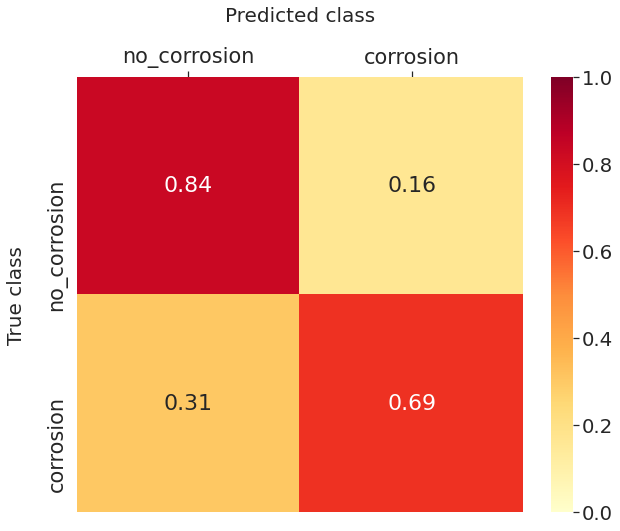
\includegraphics[width=9cm]{images/SimpleArchMatrix.png} }}%
    \end{adjustbox}
    \label{fig:simple-arch-matrix}
    \caption{\textit{Confusion Matrix} dla samodzielnie stworzonej sieci i zdjęć o rozmiarach 320x240 pikseli}
\end{figure}

\par\noindent Uzyskane wyniki pozwoliły przypuszczać, że sieci konwolucyjne są w stanie nauczyć się rozpoznawać zdjęcia ze zbioru. Były one jednak zbyt niskie, by sieć ta mogła być wykorzystana w końcowym produkcie (przede wszystkim ze względu na liczbę wyników fałszywie negatywnych, stanowiących 31\% wyników sieci dla klasy pozytywnej), dlatego zdecydowano się na próbę wytrenowania znanych architektur, których skuteczność została potwierdzona na innych zbiorach danych.


\subsubsection{Pierwsze wykorzystanie znanych architektur}

\par\noindent W pracy zdecydowano się wykorzystać architektury ResNet, Inception oraz EfficientNet. Sieć ResNet dostępna jest w wersjach posiadających różną liczbę warstw konwolucyjnych: 50, 101 oraz 152 - w pracy wykorzystano sieć posiadającą 50 warstw w wersji drugiej (V2). Sieć EfficientNet dostępna jest w wersjach B0-B7, w zależności od liczby parametrów - w pracy zbadano jakość klasyfikacji dokonywanej przez architektury B0, B3 i B7. Sieć Inception dostępna jest w wersji V3.
\par Zdjęcia znajdujące się w zbiorze danych początkowo posiadały rozdzielczość 640x480 pikseli. Został stworzony drugi zbiór, zawierający zdjęcia 2 razy mniejsze, tj. o rozdzielczości 320x240 pikseli. W początkowym podejściu do treningów z wykorzystaniem znanych architektur postanowiono zbadać, który rozmiar zdjęć skutkuje lepszą jakością klasyfikacji.
\par Każda z sieci trenowana była przez 40 epok. Podczas treningu zapisywane były wagi sieci, przy których osiągnięte zostały najwyższe do danego momentu wyniki miar jakości (accuracy, loss, precision, recall, auc) na zbiorze walidacyjnym. Po zakończeniu treningu wybierany był najlepszy model spośród zapisanych (ze względu na losową inicjalizację wag czasami uzyskane wyniki były niezadowalające - w takim przypadku trening sieci był powtarzany. Treningi powtarzano maksymalnie 3 razy i wybierano najlepszą sieć spośród wytrenowanych). Prezentowane wyniki dla wybranego modelu zostały uzyskane na zbiorze testowym.
\par Wykorzystano implementacje sieci z \textit{tf.keras.applications} z parametrem \textit{include\_top}=False. Za tym fragmentem sieci umieszczono warstwę GlobalMaxPooling2D, a następnie pojedynczą warstwę Dense. Funkcją aktywacji użytą w ostatniej warstwie był w tym przypadku sigmoid. Zdjęcie przydzielane było do klasy, która uzyskała wyższą wartość neuronu na wyjściu z ostatniej warstwy.
\vspace{3mm}
\par\noindent Zdjęcia o rozmiarach 640x480 pikseli:
\renewcommand{\arraystretch}{1.75}
 \begin{longtable}[h!]{|m{2.6cm}|m{1.2cm}|m{1.2cm}|m{1.2cm}|m{1.2cm}|m{1.2cm}|m{1.2cm}|m{1.2cm}|m{1.2cm}|}
 \hline
 Architektura & Acc & Loss & TP & FP & TN & FN & Prec & Rec\\
 \hline
 ResNet & 0.69 & 0.62 & 570 & 246 & 320 & 148 & 0.70 & 0.80\\
 \hline
 Inception & 0.73 & 0.53 & 490 & 119 & 447 & 228 & 0.80 & 0.68\\
 \hline
 EfficientNetB0 & 0.44 & 0.69 & 0 & 0 & 566 & 718 & - & 0\\
 \hline
 EfficientNetB3 & 0.44 & 0.69 & 0 & 0 & 566 & 718 & - & 0\\
 \hline
 EfficientNetB7 & 0.44 & 0.69 & 0 & 0 & 566 & 718 & - & 0\\
 \hline
 \caption{Miary jakości sieci dla różnych architektur trenowanych na zbiorze zdjęć o rozmiarach 640x480 pikseli}
 \label{table:9}
\end{longtable}

\par\noindent Znormalizowane tabele \textit{confusion matrix} dla powyższych sieci:
\begin{figure}[h!]%
    \begin{adjustbox}{minipage=1.0\paperwidth, pagecenter}
    \centering
    \subfloat[\centering ResNet]{{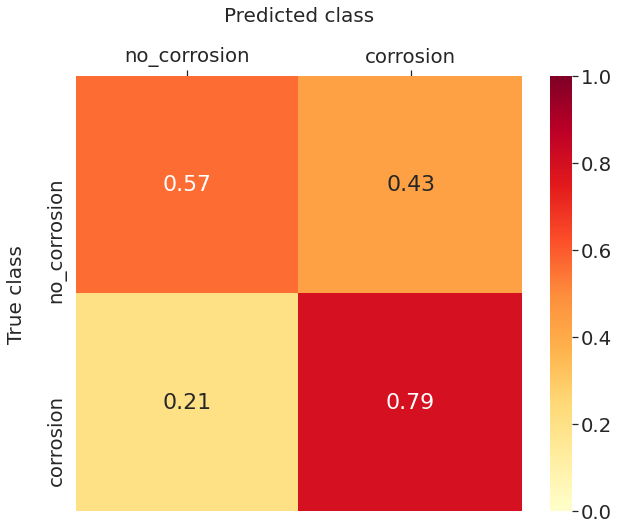
\includegraphics[width=9.cm]{images/ResNet_sigmoid_640.png} }}%
    \qquad
    \subfloat[\centering Inception]{{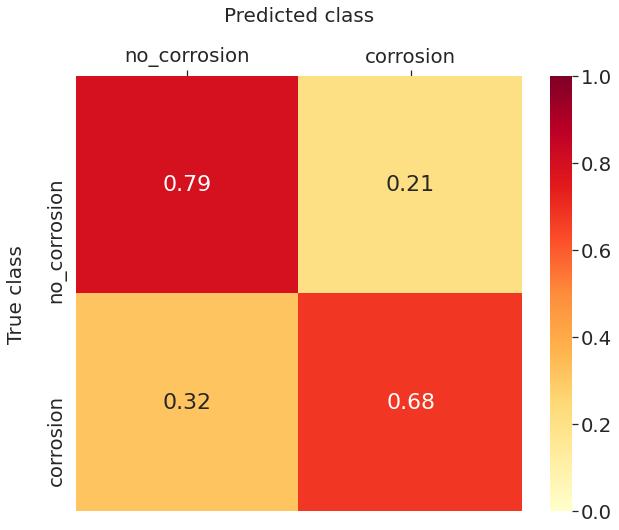
\includegraphics[width=9cm]{images/Inception_sigmoid_640.png} }}%
    \end{adjustbox}
\end{figure}
\begin{figure}[h!]%
    \ContinuedFloat
    \begin{adjustbox}{minipage=1.0\paperwidth, pagecenter}
    \centering
    \subfloat[\centering EfficientNetB0, EfficientNetB3, EfficientNetB7 (takie same wyniki)]{{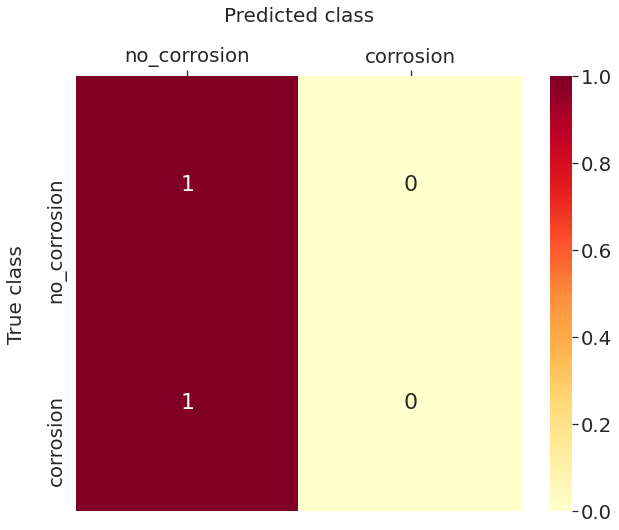
\includegraphics[width=9cm]{images/EfficientNets_sigmoid_640.png} }}%
    \end{adjustbox}
    \label{fig:sigmoid-640-480-matrices}
    \caption{Tabele \textit{confusion matrix} dla różnych architektur trenowanych na zbiorze zdjęć o rozmiarach 640x480 pikseli}
\end{figure}

\par\noindent Zdjęcia o rozmiarach 320x240 pikseli:
\renewcommand{\arraystretch}{1.6}
 \begin{longtable}[h!]{|m{2.6cm}|m{1.2cm}|m{1.2cm}|m{1.2cm}|m{1.2cm}|m{1.2cm}|m{1.2cm}|m{1.2cm}|m{1.2cm}|}
 \hline
 Architektura & Acc & Loss & TP & FP & TN & FN & Prec & Rec\\
 \hline
 ResNet & 0.77 & 0.48 & 572 & 155 & 411 & 146 & 0.79 & 0.80\\
 \hline
 Inception & 0.76 & 0.48 & 539 & 130 & 436 & 179 & 0.81 & 0.75\\
 \hline
 EfficientNetB0 & 0.75 & 0.50 & 546 & 149 & 417 & 172 & 0.79 & 0.76\\
 \hline
 EfficientNetB3 & 0.69 & 0.57 & 545 & 230 & 336 & 173 & 0.70 & 0.76 \\
 \hline
 EfficientNetB7 & 0.44 & 0.69 & 0 & 0 & 566 & 718 & - & 0 \\
 \hline
\caption{Miary jakości sieci dla różnych architektur trenowanych na zbiorze zdjęć o rozmiarach 320x240 pikseli}
\label{table:10}
\end{longtable}

\noindent Znormalizowane tabele \textit{confusion matrix} dla powyższych sieci:
\begin{figure}[H]%
    \begin{adjustbox}{minipage=1.0\paperwidth, pagecenter}
    \centering
    \subfloat[\centering ResNet]{{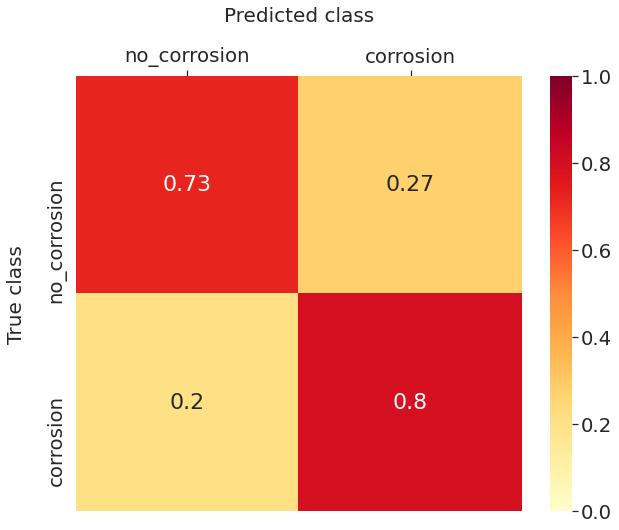
\includegraphics[width=9cm]{images/ResNet_sigmoid_320.png} }}%
    \qquad
    \subfloat[\centering Inception]{{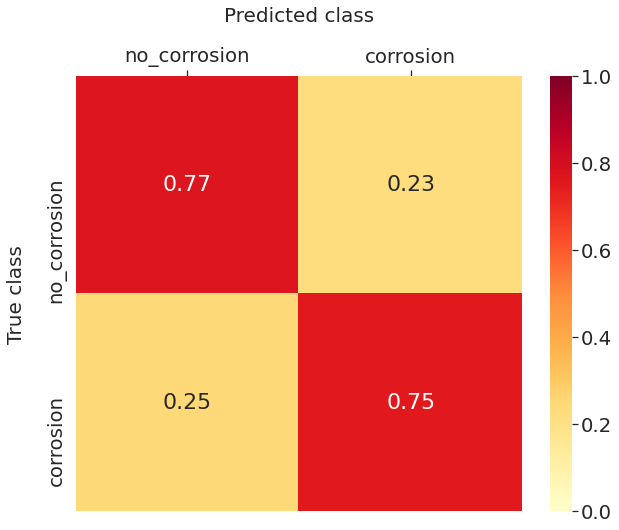
\includegraphics[width=9cm]{images/Inception_sigmoid_320.png} }}%
    \end{adjustbox}
\end{figure}
\begin{figure}[H]%
    \ContinuedFloat
    \begin{adjustbox}{minipage=1.0\paperwidth, pagecenter}
    \centering
    \subfloat[\centering EfficientNetB0]{{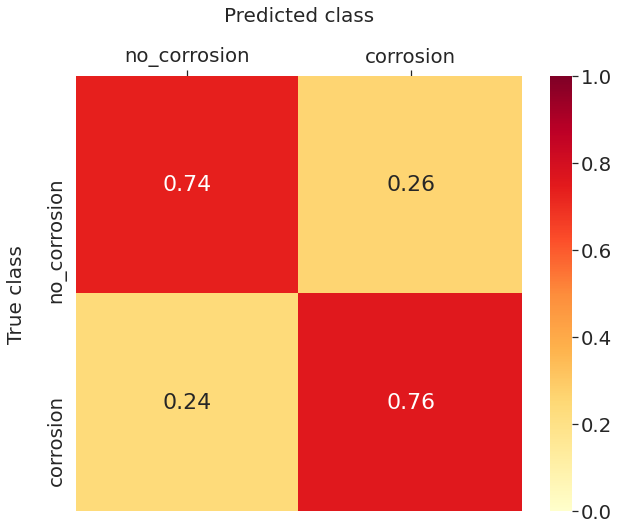
\includegraphics[width=9cm]{images/EfficientNetB0_sigmoid_320.png} }}%
    \qquad
    \subfloat[\centering EfficientNetB3]{{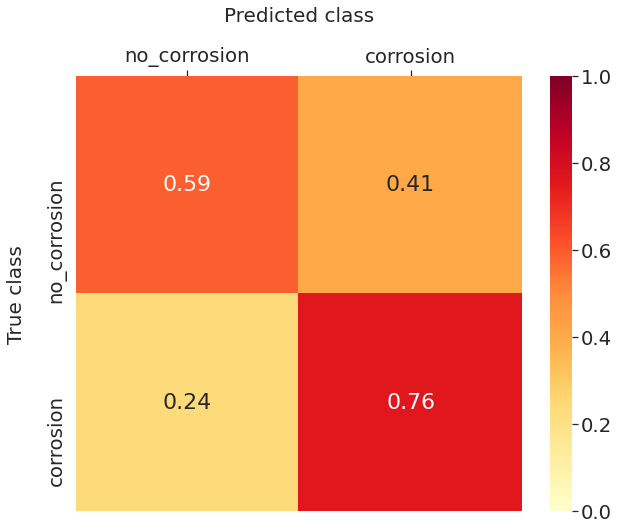
\includegraphics[width=9cm]{images/EfficientNetB3_sigmoid_320.png} }}%
    \end{adjustbox}
\end{figure}
\begin{figure}[h!]%
    \ContinuedFloat
    \begin{adjustbox}{minipage=1.0\paperwidth, pagecenter}
    \centering
    \subfloat[\centering EfficientNetB7]{{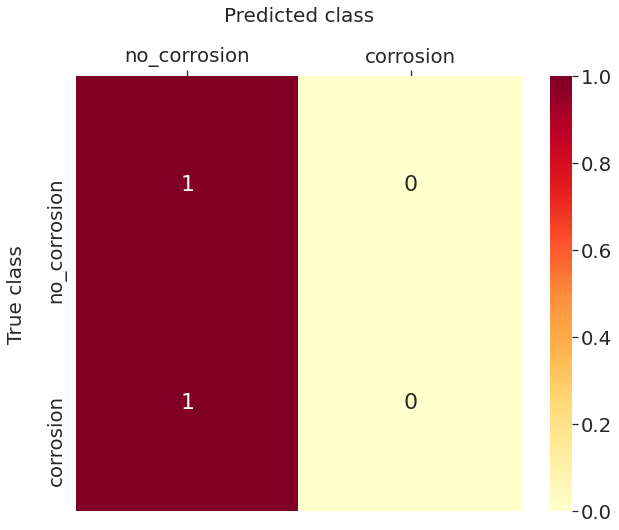
\includegraphics[width=9cm]{images/EfficientNetB7_sigmoid_320.png} }}%
    \end{adjustbox}
    \label{fig:sigmoid-320-240-matrices}
    \caption{Tabele \textit{confusion matrix} dla różnych architektur trenowanych na zbiorze zdjęć o rozmiarach 320x240 pikseli}
\end{figure}

\par Jak wynika z porównania miar jakości dla sieci trenowanych na zdjęciach o rozmiarach 640x480 pikseli względem sieci trenowanych na zdjęciach o rozmiarach 320x240 pikseli, lepszą jakość klasyfikacji uzyskano dla zdjęć o mniejszych rozmiarach. Takie rezultaty są konsekwencją niedużych rozmiarów zbioru treningowego. Sieci przy większych zdjęciach ulegają przeuczeniu się na zbiorze treningowym, w związku z czym maleje ich zdolność do generalizacji, czego skutkiem są słabe wyniki miar jakości na zbiorze testowym.
\par W przypadku zdjęć o rozmiarach 640x480 pikseli uzyskane wyniki są niezadowalające. Wszystkie testowane architektury EfficientNet podczas testów przydzieliły cały zbiór testowy do klasy ``brak korozji''. Lepszą jakość klasyfikacji pozwoliły uzyskać sieci ResNet i Inception, są to jednak również wyniki słabe - najwyższe accuracy uzyskano dla sieci Inception (73\%), jednak sieć ta zaklasyfikowała 32\% przykładów z klasy ``korozja'' do klasy ``brak korozji'', co w przypadku problemu klasyfikacji poszycia samolotów dyskwalifikuje sieć dla praktycznego wykorzystania. Wytrenowana sieć ResNet lepiej poradziła sobie z klasyfikacją zdjęć należących do klasy pozytywnej (79\% vs 21\%), jednak 21\% źle zaklasyfikowanych zdjęć z korozją to wciąż zdecydowanie zbyt duża liczba. Dodatkowo, sieć gorzej poradziła sobie z klasyfikacją przykładów należących do klasy negatywnej, zaś końcowe \textit{accuracy} (69\%) jest również niezadowalające.
\par W przypadku zdjęć o rozmiarach 320x240 pikseli wyniki są lepsze. Najlepiej z zadaniem poradziły sobie sieci ResNet, Inception oraz EfficientNetB0. W przypadku architektur EfficientNet wzrost liczby parametrów (oznaczany rosnącymi indeksami: 0, 3, 7) powodował spadek jakości klasyfikacji - parametrów było zbyt dużo względem rozmiaru zbioru treningowego i sieć ulegała przeuczeniu na tym zbiorze, co skutkowało niską jakością klasyfikacji na zbiorze testowym. Osiągnięte wyniki w przypadku pozostałych architektur dobrze rokowały na przyszłość w kwestii ich wykorzystania w ostatecznie wybranym klasyfikatorze, jednak zarówno osiągnięte \textit{accuracy} (odpowiednio 77\%, 76\% i 75\% dla sieci ResNet, Inception i EfficientNetB0) jak i znormalizowana liczba wyników fałszywie negatywnych (odpowiednio 20\%, 25\%, 24\%) nie były zadowalające. Warto dodać, że wymienione sieci porównywalnie radzą sobie z rozpoznawaniem zarówno klasy pozytywnej jak i negatywnej.
\par Należy podkreślić, że problem minimalizacji liczby wyników fałszywie negatywnych (lewa dolna ćwiartka w tabelach \textit{confusion matrix}) ma krytyczne znaczenie w problemie klasyfikacji poszycia statków powietrznych pod kątem występowania na nim korozji. Pominięcie naprawy zniszczonego fragmentu samolotu może mieć tragiczne skutki dla bezpieczeństwa pasażerów maszyny. Ponieważ powyższe modele generują zbyt dużą liczbę wyników fałszywie negatywnych, kolejnym sposobem podejścia do problemu została próba dostosowania progu, od którego zdjęcie było przydzielane do klasy pozytywnej.

\subsubsection{Manipulacja progiem przydzielania zdjęć do klasy pozytywnej}
\par\noindent  
W celu zmniejszenia liczby wyników fałszywie negatywnych ponownie wytrenowano sieci bazujące na najlepiej sprawujących się w poprzednim doświadczeniu architekturach (ResNet, Inception, EfficientNetB0) oraz zdjęciach o rozmiarze dostarczającym lepszej jakości klasyfikacji - 320x240 pikseli, tym razem używając funkcji softmax jako funkcji aktywacji neuronów ostatniej warstwy (softmax dostarcza prawdopodobieństwa przynależności klasyfikowanego wejścia do każdej klasy, a ich suma wynosi 1.0. Używany jest, gdy klasy się wzajemnie wykluczają, tak jak w przypadku analizowanego zbioru, w którym zdjęcie jest jednoznacznie klasyfikowane jako skorodowane albo nieskorodowane. Zwiększenie prawdopodobieństwa przynależności do jednej z klas automatycznie zmniejsza prawdopodobieństwo pozostałych). Podczas ewaluacji modeli na zbiorze testowym zdjęcia przydzielane były do klasy pozytywnej, gdy wartość neuronu z ostatniej warstwy dla klasy pozytywnej była większa niż zdefiniowany próg (domyślnie jest to 0.5), zaś pozostałe zdjęcia trafiały do klasy negatywnej (brak korozji). Do analizy wpływu przesunięcia progu na poprawę klasyfikacji przetestowano wartości: 0.5, 0.45, 0.4, 0.35, 0.3 oraz 0.25.

Do oceny jakości wybranego progu pod uwagę zostały wzięte: \textit{accuracy}, \textit{precision}, \textit{recall} oraz \textit{F1 score}. \textit{F1 score} jest średnią harmoniczną \textit{precision} oraz \textit{recall}. Przy zmniejszaniu progu dla klasy pozytywnej osiągany jest pożądany efekt zmniejszenia się liczby wyników fałszywie negatywnych, jednak możliwe, że w takim procesie gwałtownie obniżona zostanie wartość \textit{precision}, dlatego ważne jest kontrolowanie wartości obu miar klasyfikacji \textit{precision} i \textit{recall}, co umożliwia miara \textit{F1 score}.

\vspace{3mm}
\par\noindent Poniżej przedstawiono wyniki tego eksperymentu:
\vspace{3mm}
\par\noindent ResNet:
 \begin{longtable}[h!]{|m{2.0cm}|m{1.2cm}|m{1.2cm}|m{1.2cm}|m{1.2cm}|m{1.2cm}|m{1.2cm}|m{1.2cm}|m{1.6cm}|}
 \hline
 Próg & Acc & TP & FP & TN & FN & Prec & Rec & F1 score\\
 \hline
 0.5 & 0.71 & 429 & 84 & 482 & 289 & 0.84 & 0.60 & 0.70\\
 \hline
 0.45 & 0.71 & 467 & 117 & 449 & 251 & 0.80 & 0.65 & 0.72\\
 \hline
 0.4 & 0.71 & 498 & 150 & 416 & 220 & 0.77 & 0.69 & 0.73\\
 \hline
 0.35 & 0.70 & 530 & 192 & 374 & 188 & 0.73 & 0.74 & 0.74 \\
 \hline
 0.3 & 0.71 & 568 & 228 & 338 & 150 & 0.71 & 0.79 & 0.75\\
 \hline
 0.25 & 0.69 & 605 & 286 & 280 & 113 & 0.68 & 0.84 & 0.75\\
 \hline
\caption{Miary jakości sieci ResNet dla różnych progów dla klasy pozytywnej na zbiorze zdjęć o rozmiarach 320x240 pikseli}
\label{table:11}
\end{longtable}

\begin{figure}[h!]
    \begin{adjustbox}{minipage=1.0\paperwidth, pagecenter}
    \centering
    \subfloat[\centering Confusion matrix dla sieci ResNet dla domyślnego progu - 0.5]{{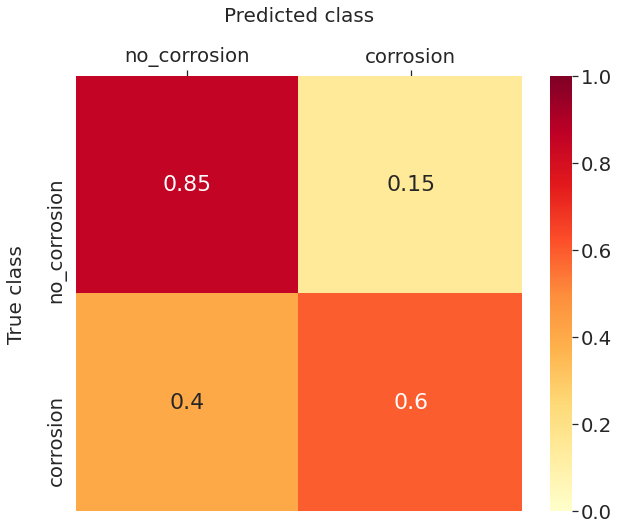
\includegraphics[width=9cm, height=8cm]{images/ResNet_softmax_0,5.png} }}%
    \qquad
    \subfloat[\centering Confusion matrix dla sieci ResNet dla progu 0.3]{{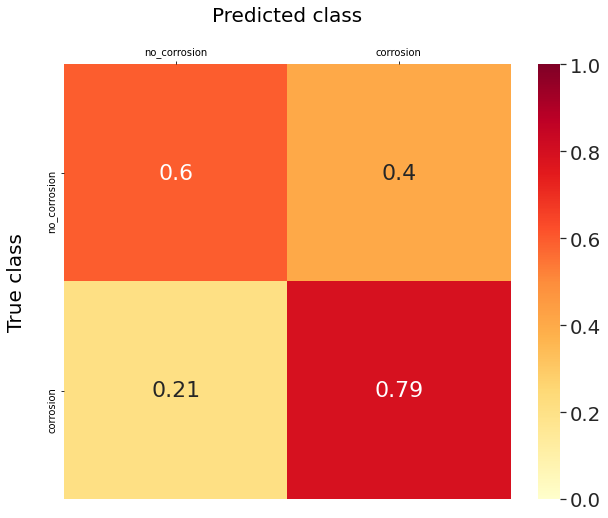
\includegraphics[width=9cm, height=8cm]{images/ResNet_softmax_0,3.png} }}%
    \end{adjustbox}
    \label{fig:resnet-softmax-matrices}
    \caption{Znormalizowane tabele \textit{confusion matrix} dla sieci ResNet}
\end{figure}

\par\noindent Inception:
 \begin{longtable}[h!]{|m{2.0cm}|m{1.2cm}|m{1.2cm}|m{1.2cm}|m{1.2cm}|m{1.2cm}|m{1.2cm}|m{1.2cm}|m{1.6cm}|}
 \hline
 Próg & Acc & TP & FP & TN & FN & Prec & Rec & F1 score\\
 \hline
 0.5 & 0.73 & 603 & 231 & 335 & 115 & 0.72 & 0.84 & 0.78\\
 \hline
 0.45 & 0.73 & 631 & 256 & 310 & 87 & 0.71 & 0.88 & 0.79\\
 \hline
 0.4 & 0.72 & 642 & 278 & 288 & 76 & 0.70 & 0.89 & 0.78\\
 \hline
 0.35 & 0.72 & 659 & 304 & 262 & 59 & 0.68 & 0.92 & 0.78 \\
 \hline
 0.3 & 0.70 & 670 & 337 & 229 & 48 & 0.67 & 0.93 & 0.78\\
 \hline
 0.25 & 0.69 & 690 & 366 & 200 & 28 & 0.65 & 0.96 & 0.78\\
 \hline
\caption{Miary jakości sieci Inception dla różnych progów dla klasy pozytywnej na zbiorze zdjęć o rozmiarach 320x240 pikseli}
\label{table:12}
\end{longtable}

\begin{figure}[h!]
    \begin{adjustbox}{minipage=1.0\paperwidth, pagecenter}
    \centering
    \subfloat[\centering Confusion matrix dla sieci Inception dla domyślnego progu - 0.5]{{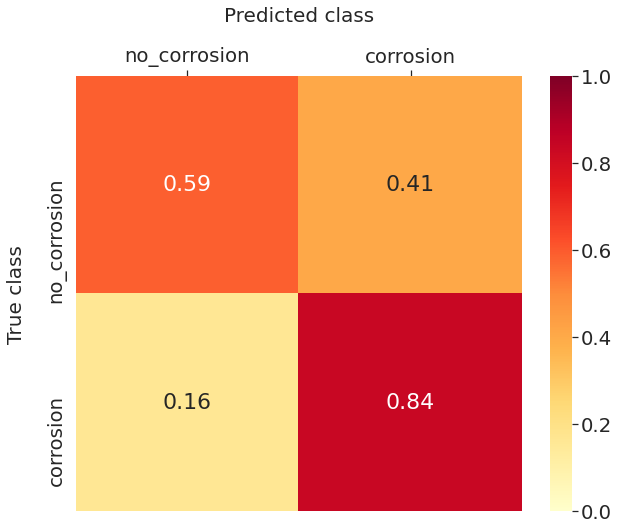
\includegraphics[width=9cm]{images/Inc_softmax_0,5.png} }}%
    \qquad
    \subfloat[\centering Confusion matrix dla sieci Inception dla najlepszego progu - 0.35]{{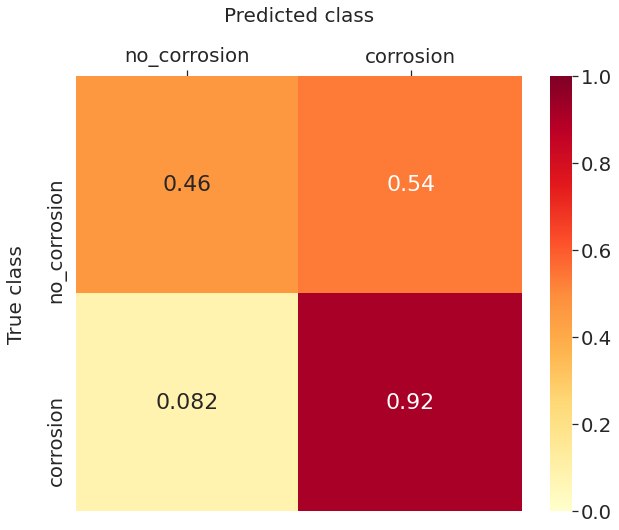
\includegraphics[width=9cm]{images/Inc_softmax_0,35.png} }}%
    \end{adjustbox}
    \label{fig:inception-softmax-matrices}
    \caption{Znormalizowane tabele \textit{confusion matrix} dla sieci Inception}
\end{figure}

\par\noindent EfficientNetB0:
 \begin{longtable}[h!]{|m{2.0cm}|m{1.2cm}|m{1.2cm}|m{1.2cm}|m{1.2cm}|m{1.2cm}|m{1.2cm}|m{1.2cm}|m{1.6cm}|}
 \hline
 Próg & Acc & TP & FP & TN & FN & Prec & Rec & F1 score\\
 \hline
 0.5 & 0.71 & 445 & 93 & 473 & 273 & 0.83 & 0.62 & 0.71\\
 \hline
 0.45 & 0.73 & 485 & 119 & 447 & 233 & 0.80 & 0.68 & 0.73\\
 \hline
 0.4 & 0.73 & 520 & 149 & 417 & 198 & 0.78 & 0.72 & 0.75\\
 \hline
 0.35 & 0.73 & 558 & 190 & 376 & 160 & 0.75 & 0.78 & 0.76 \\
 \hline
 0.3 & 0.72 & 584 & 228 & 338 & 134 & 0.72 & 0.81 & 0.76\\
 \hline
 0.25 & 0.72 & 634 & 274 & 292 & 84 & 0.70 & 0.88 & 0.78\\
 \hline
\caption{Miary jakości sieci EfficientNetB0 dla różnych progów dla klasy pozytywnej na zbiorze zdjęć o rozmiarach 320x240 pikseli}
\end{longtable}

\begin{figure}[h!]
    \begin{adjustbox}{minipage=1.0\paperwidth, pagecenter}
    \centering
    \subfloat[\centering Confusion matrix dla sieci EfficientNetB0 dla domyślnego progu - 0.5]{{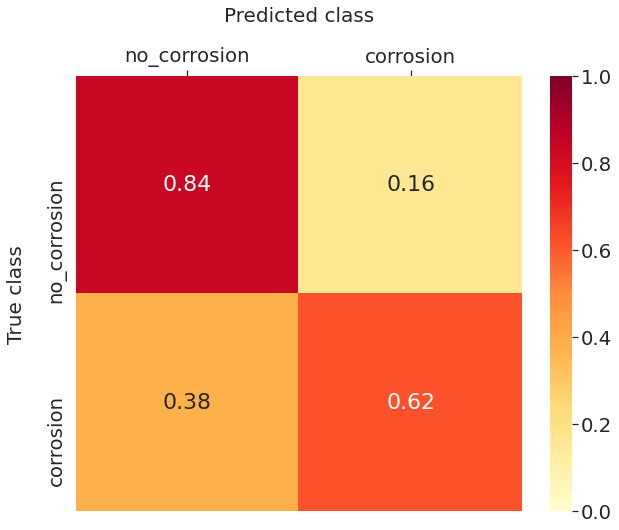
\includegraphics[width=9cm]{images/EffB0_softmax_0,5.png} }}%
    \qquad
    \subfloat[\centering Confusion matrix dla sieci EfficientNetB0 dla najlepszego progu - 0.25]{{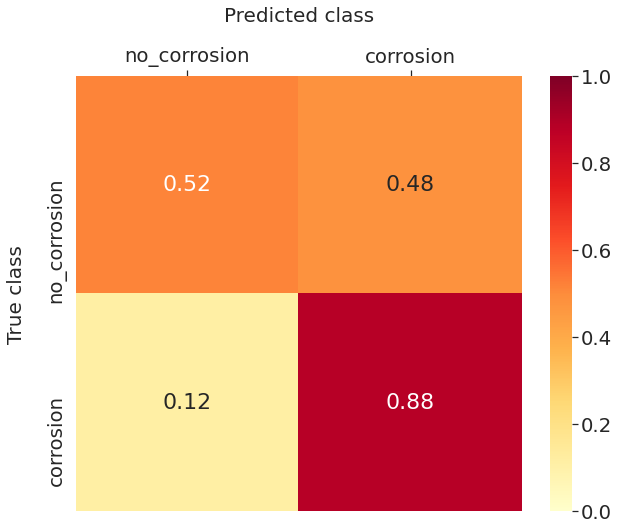
\includegraphics[width=9cm]{images/EffB0_softmax_0,25.png} }}%
    \end{adjustbox}
    \label{fig:effnetb0-softmax-matrices}
    \caption{Znormalizowane tabele \textit{confusion matrix} dla sieci EfficientNetB0}
    \label{table:13}
\end{figure}

\par Powyższa manipulacja progiem przydzielania zdjęć do klasy pozytywnej pozwoliła na wykazanie, że jest to skuteczna metoda redukcji liczby zdjęć zaklasyfikowanych niepoprawnie do klasy negatywnej. W przypadku EfficientNetB0 obniżanie progu przynależności do klasy pozytywnej zwiększyło \textit{accuracy} w stosunku do domyślnego progu 0.5. W przypadku wszystkich testowanych sieci manipulacja zwiększała \textit{recall} przy jednoczesnym obniżeniu \textit{precision}, co było oczekiwanym efektem. Dla sieci Inception zmiana wartości \textit{recall} i \textit{precision} była najmniejsza - dla najlepszego wybranego progu 0.35 \textit{precision} zmalało o 4 p.p., a \textit{recall} zwiększył się o 8 p.p. Sieć ResNet przy progu 0.3 uzyskała \textit{precision} zmniejszone o 13 p.p., a \textit{recall} zwiększony o 19 p.p. W przypadku EfficientNetB0 przy progu 0.25 wartość \textit{precision} zmniejszyła się o tyle samo, co dla sieci ResNet (13 p.p.), a \textit{recall} zwiększył się o 26 p.p. 

ResNet oraz EfficientNetB0 przy domyślnym progu miały porównywalne wartości \textit{precision} oraz \textit{recall}, a po manipulacji progiem lepsze miary jakości uzyskiwał EfficientNetB0 (poprawiło się również \textit{accuracy}). 
Z trzech modeli Inception był jedynym, dla którego \textit{recall} był większy od \textit{precision} przy domyślnym progu, dlatego dalsza manipulacja powiększyła \textit{recall} do dużych wartości - dla najlepszego progu 0.35 wyniósł on 92\%.

Dla testowanych modeli nie udało się znaleźć progu, przy którym jednocześnie liczba \textit{false negativów} będzie niska i nie zwiększy się drastycznie liczba \textit{false positivów}.

\subsubsection{Ekstrakcja cech obrazów i klasyfikacja z wykorzystaniem SVM}

\par W pracy postanowiono również przeprowadzić eksperyment polegający na potraktowaniu fragmentu wytrenowanej sieci neuronowej (wziętej od jej wejścia do wyjścia aktywacji za ostatnią warstwą konwolucyjną) jako ekstraktora cech obrazów, które następnie klasyfikowane były przy pomocy SVM na podstawie wyekstrahowanych cech.
\par Zbiór treningowy został przepuszczony przez wybraną część sieci w 1000-elementowych batchach, następnie zmniejszono wymiarowość zbioru do 100 (ze względu na bardzo dużą pierwotną liczbę wymiarów: 8*10*2048=163840 dla sieci ResNet, 6*8*2048=98304 dla sieci Inception i 8*10*1280=102400 dla EfficientNetB0, powodującą przekroczenie dostępnej pamięci przy jednoczesnej alokacji całego zbioru) za pomocą PCA i tak przetworzony zbiór (po połączeniu poszczególnych batchy w jeden zbiór) został podany klasyfikatorowi SVM do treningu. Podobnie przetworzono zbiór testowy.
\par Do ekstrakcji cech wykorzystano wytrenowane wcześniej sieci o architekturach ResNet, Inception i EfficientNetB0, wykorzystujące jako funkcję aktywacji neuronów ostatniej, gęstej warstwy (znajdującej się już poza fragmentem sieci wykorzystywanym do ekstrakcji cech) sigmoid albo softmax.
\par Wykorzystano implementację SVM z biblioteki sklearn, przetestowano kernele linear, poly, rbf i sigmoid. Pozostałe parametry posiadały domyślne wartości.
\vspace{3mm}
\par\noindent Poniżej znajdują się wyniki ewaluacji klasyfikatorów na zbiorze testowym:
\vspace{3mm}
\newline\noindent ResNet:
 \begin{longtable}[h!]{|m{1.9cm}|m{1.5cm}|m{1.2cm}|m{1.2cm}|m{1.2cm}|m{1.2cm}|m{1.2cm}|m{1.2cm}|m{1.2cm}|m{1.2cm}|}
 \hline
 Aktywacja & Kernel & Acc & TP & FP & TN & FN & Prec & Rec\\
 \hline
 Sigmoid & RBF & 0.56 & 717 & 565 & 1 & 1 & 0.56 & 1.0\\
 \hline
 Sigmoid & Linear & 0.74 & 455 & 66 & 500 & 263 & 0.87 & 0.63\\
 \hline
 Sigmoid & Poly & 0.56 & 718 & 566 & 0 & 0 & 0.56 & 1.0\\
 \hline
 Sigmoid & Sigmoid & 0.56 & 717 & 564 & 2 & 1 & 0.56 & 1.0\\
 \hline
 Softmax & RBF & 0.58 & 202 & 19 & 547 & 516 & 0.91 & 0.28\\
 \hline
 Softmax & Linear & 0.68 & 381 & 70 & 496 & 337 & 0.84 & 0.53\\
 \hline
 Softmax & Poly & 0.56 & 718 & 566 & 0 & 0 & 0.56 & 1.0\\
 \hline
 Softmax & Sigmoid & 0.46 & 34 & 3 & 563 & 684 & 0.92 & 0.05\\
 \hline
\caption{Miary jakości sieci klasyfikatora SVM dla ekstraktora cech opartego o sieć ResNet}
\label{table:14}
\end{longtable}

\noindent Inception:
 \begin{longtable}[h!]{|m{1.9cm}|m{1.5cm}|m{1.2cm}|m{1.2cm}|m{1.2cm}|m{1.2cm}|m{1.2cm}|m{1.2cm}|m{1.2cm}|m{1.2cm}|}
 \hline
 Aktywacja & Kernel & Acc & TP & FP & TN & FN & Prec & Rec\\
 \hline
 Sigmoid & RBF & 0.74 & 491 & 110 & 456 & 227 & 0.82 & 0.68\\
 \hline
 Sigmoid & Linear & 0.75 & 509 & 110 & 456 & 209 & 0.82 & 0.71\\
 \hline
 Sigmoid & Poly & 0.71 & 385 & 43 & 523 & 333 & 0.90 & 0.54\\
 \hline
 Sigmoid & Sigmoid & 0.66 & 451 & 165 & 401 & 267 & 0.73 & 0.63\\
 \hline
 Softmax & RBF & 0.75 & 508 & 116 & 450 & 210 & 0.81 & 0.71\\
 \hline
 Softmax & Linear & 0.75 & 498 & 104 & 462 & 220 & 0.83 & 0.69\\
 \hline
 Softmax & Poly & 0.72 & 412 & 50 & 516 & 306 & 0.89 & 0.57\\
 \hline
 Softmax & Sigmoid & 0.68 & 469 & 159 & 407 & 249 & 0.75 & 0.65\\
 \hline
\caption{Miary jakości sieci klasyfikatora SVM dla ekstraktora cech opartego o sieć Inception}
\label{table:15}
\end{longtable}

\noindent EfficientNetB0:
 \begin{longtable}[h!]{|m{1.9cm}|m{1.5cm}|m{1.2cm}|m{1.2cm}|m{1.2cm}|m{1.2cm}|m{1.2cm}|m{1.2cm}|m{1.2cm}|m{1.2cm}|}
 \hline
 Aktywacja & Kernel & Acc & TP & FP & TN & FN & Prec & Rec\\
 \hline
 Sigmoid & RBF & 0.73 & 453 & 87 & 479 & 265 & 0.84 & 0.63\\
 \hline
 Sigmoid & Linear & 0.74 & 482 & 99 & 467 & 236 & 0.83 & 0.67\\
 \hline
 Sigmoid & Poly & 0.56 & 718 & 566 & 0 & 0 & 0.56 & 1.0\\
 \hline
 Sigmoid & Sigmoid & 0.74 & 491 & 108 & 458 & 227 & 0.82 & 0.68\\
 \hline
 Softmax & RBF & 0.73 & 457 & 80 & 486 & 261 & 0.85 & 0.64\\
 \hline
 Softmax & Linear & 0.74 & 473 & 88 & 478 & 245 & 0.84 & 0.66\\
 \hline
 Softmax & Poly & 0.56 & 718 & 566 & 0 & 0 & 0.56 & 1.0\\
 \hline
 Softmax & Sigmoid & 0.74 & 478 & 90 & 476 & 240 & 0.84 & 0.67\\
 \hline
\caption{Miary jakości sieci klasyfikatora SVM dla ekstraktora cech opartego o sieć EfficientNetB0}
\label{table:16}
\end{longtable}

\par Klasyfikatory, które uzyskały wysokie \textit{accuracy} i jednocześnie najwyższe wartości \textit{recall}, to klasyfikatory z ekstraktorami cech opartymi o sieć Inception: Inception-Sigmoid-Linear oraz Inception-Softmax-RBF (architektura sieci będącej ekstraktorem cech-funkcja aktywacji ostatniej warstwy pełnej sieci-kernel klasyfikatora SVM).

\noindent Znormalizowane tablice confusion matrix dla powyższych klasyfikatorów:
\begin{figure}[H]%
    \begin{adjustbox}{minipage=1.0\paperwidth, pagecenter}
    \centering
    \subfloat[\centering Confusion matrix dla klasyfikatora Inception-Sigmoid-Linear]{{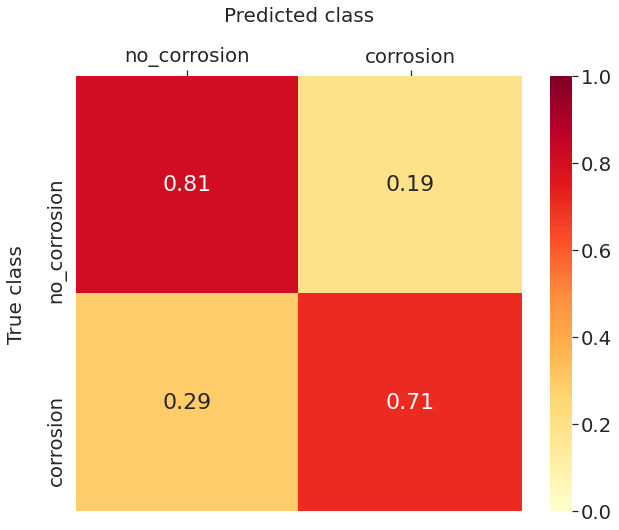
\includegraphics[width=9cm]{images/incSigmLin.png} }}%
    \qquad
    \subfloat[\centering Confusion matrix dla klasyfikatora Inception-Softmax-RBF]{{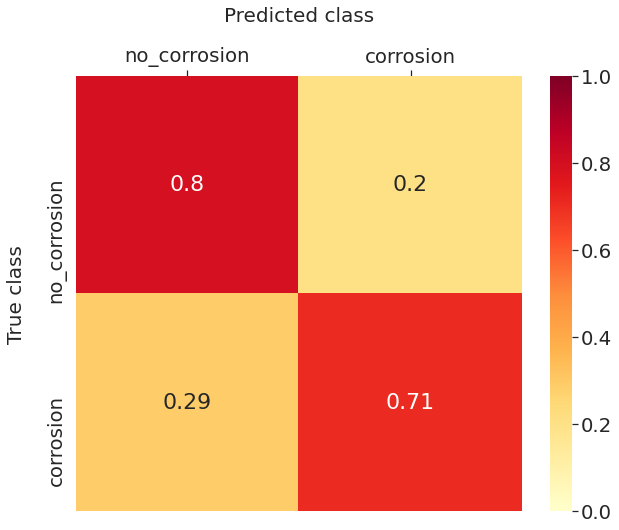
\includegraphics[width=9cm]{images/incSoftRBF.png} }}%
    \end{adjustbox}
    \label{fig:svm-matrices}
    \caption{Tabele \textit{confusion matrix} dla klasyfikacji z wykorzystaniem SVM}
\end{figure}

\par Niektóre klasyfikatory osiągnęły \textit{accuracy} porównywalne z wynikami sieci, na bazie których powstały wykorzystane przez nie ekstraktory cech - najwyższe poziomy \textit{accuracy} uzyskane w eksperymencie to 74-75\%, zaś dla pełnych sieci są to odpowiednio 75-77\% dla sieci z sigmoidą oraz 71-73\% dla sieci z softmaxem. 
\par Żaden z klasyfikatorów nie radzi sobie dobrze z klasyfikacją zdjęć zawierających fragmenty skorodowane - dla najlepiej sprawujących się klasyfikatorów wyniki fałszywe stanowią 29\% wyników dla zdjęć z korozją.
\par Ze względu na niezadowalające wyniki, eksperyment z ekstrakcją cech obrazów za pomocą sieci neuronowych i klasyfikacją obrazów na podstawie wyekstrahowanych cech za pomocą klasyfikatora SVM został na tym etapie zakończony.


\subsubsection{Klasyfikatory zespołowe}
\par\noindent Ponieważ podejście wykorzystujące klasyfikator złożony z kilku podklasyfikatorów zostało udokumentowane jako przynoszące lepsze wyniki niż podejście wykorzystujące pojedynczy klasyfikator\cite{artRen}, w pracy zbadano również możliwość wykorzystania \textit{ensemble learningu} do stworzenia końcowego klasyfikatora. Zbadano architektury ResNet, Inception i EfficientNetB0 oraz klasyfikatory złożone z 3 albo 5 podsieci tego samego rodzaju. 
\newline Każda z podsieci trenowana była na innym zbiorze danych (takim samym pomiędzy podklasyfikatorami). Sprawdzono 3 różne poziomy pokrywania się ze sobą zbiorów uczących w podklasyfikatorach, oznaczone jako parametr \textit{coverage}, gdzie:
\begin{itemize}
    \item coverage=None - zbiory zdjęć przeznaczone do treningu dla podklasyfikatorów są rozłączne
    \item coverage=0.5 - każdy ze zbiorów przeznaczonych do treningu dla danego podklasyfikatora pokrywa 50\% pełnego zbioru uczącego (a więc zbiory te przecinają się)
    \item coverage=0.7 - każdy ze zbiorów przeznaczonych do treningu dla danego podklasyfikatora pokrywa 70\% pełnego zbioru uczącego (a więc zbiory te przecinają się)
\end{itemize}
Zbiór danych, podzielony na zdjęcia pochodzące z konkretnych maszyn, został podzielony tak, by każdy podklasyfikator otrzymał porównywalną liczbę zdjęć przeznaczonych do treningu. Konkretny podział na maszyny zdjęć przeznaczonych do treningu dla danego klasyfikatora przedstawiał się następująco: 
\begin{itemize}
    \item dla klasyfikatora złożonego z 3 sieci:
    \begin{itemize}
        \item Coverage=None:
        \begin{itemize}
            \item Klasyfikator 1: maszyny nr 2, 5, 6, 8, 9, 11, 12, 14, 15, 22, 23, 27
            \item Klasyfikator 2: maszyny nr 1, 3, 4, 7, 10, 18, 19, 20, 21, 25
            \item Klasyfikator 3: maszyny nr 13, 16, 17, 24, 26, 28, 29, 30
        \end{itemize}
        \item Coverage=0.5:
        \begin{itemize}
            \item Klasyfikator 1: maszyny nr 2, 5, 8, 13, 15, 17, 18, 19, 22, 23, 26, 30
            \item Klasyfikator 2: maszyny nr 1, 3, 4, 5, 6, 8, 9, 10, 17, 18, 20, 21, 22, 27, 29
            \item Klasyfikator 3: maszyny nr 1, 2, 4, 7, 9, 11, 12, 14, 16, 19, 20, 23, 24, 25, 28, 29, 30
        \end{itemize}
        \item Coverage=0.7:
        \begin{itemize}
            \item Klasyfikator 1: maszyny nr 1, 2, 3, 4, 6, 8, 9, 11, 12, 14, 17, 18, 19, 20, 21, 22, 23, 24, 27, 28, 29
            \item Klasyfikator 2: maszyny nr 1, 3, 4, 5, 7, 8, 9, 10, 11, 13, 15, 16, 17, 18, 20, 23, 24, 25, 26, 28, 29, 30
            \item Klasyfikator 3: maszyny nr 2, 4, 5, 6, 7, 9, 10, 12, 13, 14, 15, 16, 19, 21, 22, 24, 25, 26, 27, 29, 30
        \end{itemize}
    \end{itemize}
    \item dla klasyfikatora złożonego z 5 sieci:
    \begin{itemize}
        \item Coverage=None:
        \begin{itemize}
            \item Klasyfikator 1: maszyny nr 6, 8, 17, 20, 24, 25, 27
            \item Klasyfikator 2: maszyny nr 12, 15, 16, 22, 28
            \item Klasyfikator 3: maszyny nr 2, 3, 4, 18, 19, 30
            \item Klasyfikator 4: maszyny nr 7, 9, 10, 11, 13, 21, 29
            \item Klasyfikator 5: maszyny nr 1, 5, 14, 23, 26
        \end{itemize}
        \item Coverage=0.5:
        \begin{itemize}
            \item Klasyfikator 1: maszyny nr 1, 2, 3, 4, 5, 6, 8, 9, 10, 12, 14, 15, 18, 19, 20, 21, 22, 23, 26, 30
            \item Klasyfikator 2: maszyny nr 1, 3, 5, 6, 7, 8, 10, 11, 13, 15, 16, 17, 18, 19, 20, 21, 23, 24, 25, 27, 28
            \item Klasyfikator 3: maszyny nr 3, 4, 5, 7, 9, 10, 12, 13, 14, 15, 16, 17, 19, 21, 22, 23, 24, 26, 28, 29, 30
            \item Klasyfikator 4: maszyny nr 2, 3, 4, 5, 7, 8, 9, 11, 13, 14, 15, 18, 19, 20, 21, 25, 26, 27, 28, 29, 30
            \item Klasyfikator 5: maszyny nr 1, 2, 4, 5, 6, 7, 9, 11, 12, 13, 14, 15, 16, 18, 22, 23, 24, 25, 26, 27, 30
        \end{itemize}
        \item Coverage=0.7:
        \begin{itemize}
            \item Klasyfikator 1: maszyny nr 1, 2, 3, 6, 7, 8, 9, 10, 11, 12, 13, 14, 15, 18, 19, 21, 23, 26, 27, 28, 30
            \item Klasyfikator 2: maszyny nr 1, 2, 3, 4, 6, 7, 8, 10, 11, 12, 13, 15, 17, 19, 20, 21, 22, 23, 24, 25, 27, 28, 29
            \item Klasyfikator 3: maszyny nr 1, 2, 3, 4, 5, 6, 8, 9, 10, 12, 13, 14, 15, 16, 18, 20, 21, 24, 25, 28, 29, 30
            \item Klasyfikator 4: maszyny nr 1, 3, 4, 6, 7, 8, 9, 10, 11, 12, 13, 14, 16, 17, 18, 20, 22, 23, 25, 26, 27, 29, 30
            \item Klasyfikator 5: maszyny nr 4, 7, 9, 11, 12, 14, 15, 16, 19, 21, 22, 23, 24, 25, 26, 27, 29, 30
        \end{itemize}
    \end{itemize}
\end{itemize}

\par\noindent Do fuzji decyzji podklasyfikatorów wykorzystano average voting (zespół average) oraz majority voting (zespół majority).
\par\noindent Po przeprowadzeniu odpowiednich treningów uzyskano następujące wyniki:
\vspace{3mm}
\newline\noindent ResNet:
\vspace{3mm}
\newline\noindent Zespół 3 podklasyfikatorów, coverage=None:
\renewcommand{\arraystretch}{1.75}
 \begin{longtable}[h!]{|m{2.6cm}|m{1.2cm}|m{1.2cm}|m{1.2cm}|m{1.2cm}|m{1.2cm}|m{1.2cm}|m{1.2cm}|m{1.2cm}|}
 \hline
 Klasyfikator & Acc & Loss & TP & FP & TN & FN & Prec & Rec\\
 \hline
 Klasyfikator 1 & 0.65 & 0.62 & 439 & 175 & 391 & 279 & 0.71 & 0.61\\
 \hline
 Klasyfikator 2 & 0.69 & 0.89 & 182 & 217 & 349 & 536 & 0.71 & 0.75\\
 \hline
 Klasyfikator 3 & 0.62 & 0.65 & 453 & 220 & 346 & 265 & 0.67 & 0.63\\
 \hline
 Zespół average & 0.71 & 0.55 & 530 & 189 & 377 & 188 & 0.74 & 0.74\\ 
 \hline
 Zespół \newline majority & 0.70 & 1.38 & 493 & 160 & 406 & 225 & 0.75 & 0.69\\
 \hline
\caption{Miary jakości sieci dla klasyfikatorów zespołowych oraz wchodzących w ich skład podklasyfikatorów dla sieci ResNet, zespołu 3 podklasyfikatorów oraz parametru coverage=None}
\label{table:17}
\end{longtable}

\noindent Znormalizowane tabele \textit{confusion matrix} dla powyższych klasyfikatorów zespołowych:
\begin{figure}[H]%
    \begin{adjustbox}{minipage=1.0\paperwidth, pagecenter}
    \centering
    \subfloat[\centering Zespół average]{{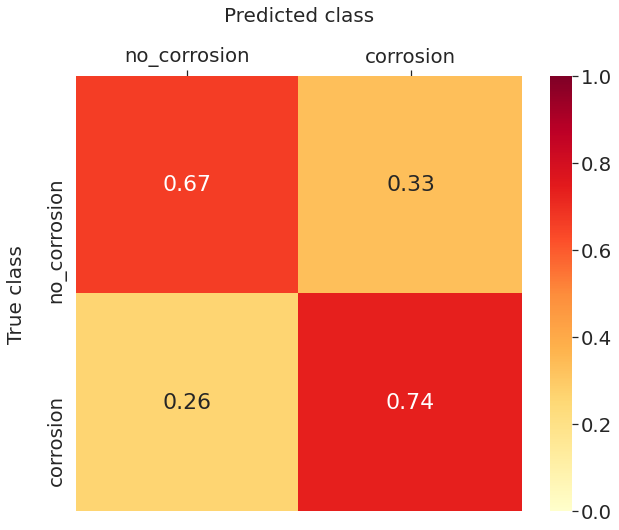
\includegraphics[width=8.7cm]{images/ResNet_ensemble_3_None_average.png} }}%
    \qquad
    \subfloat[\centering Zespół majority]{{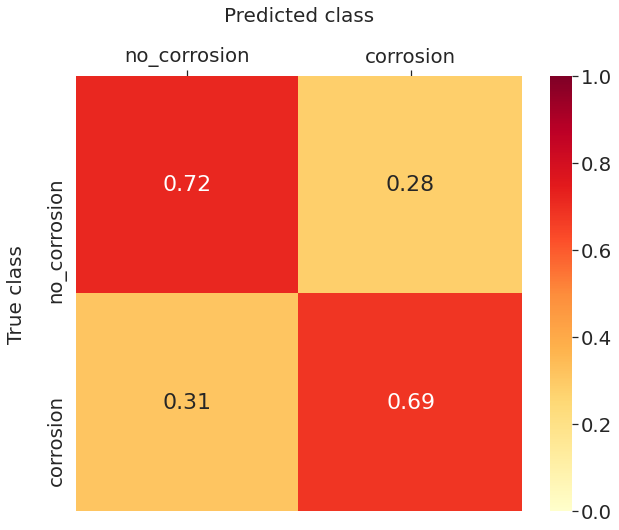
\includegraphics[width=8.7cm]{images/ResNet_ensemble_3_None_majority.png} }}%
    \end{adjustbox}
    \label{fig:resnet-ens-3-None-matrices}
    \caption{Tabele \textit{confusion matrix} dla zespołu 3 klasyfikatorów opartych o architekturę ResNet, z parametrem coverage=None}
\end{figure}
\newpage
\noindent Zespół 3 podklasyfikatorów, coverage=0.5:
 \begin{longtable}[h!]{|m{2.6cm}|m{1.2cm}|m{1.2cm}|m{1.2cm}|m{1.2cm}|m{1.2cm}|m{1.2cm}|m{1.2cm}|m{1.2cm}|}
 \hline
 Klasyfikator & Acc & Loss & TP & FP & TN & FN & Prec & Rec\\
 \hline
 Klasyfikator 1 & 0.70 & 0.57 & 527 & 193 & 373 & 191 & 0.73 & 0.73\\
 \hline
 Klasyfikator 2 & 0.67 & 0.90 & 487 & 187 & 379 & 231 & 0.72 & 0.68\\
 \hline
 Klasyfikator 3 & 0.71 & 0.59 & 588 & 247 & 319 & 130 & 0.70 & 0.82\\
 \hline
 Zespół average & 0.72 & 0.56 & 567 & 204 & 362 & 151 & 0.74 & 0.79\\ 
 \hline
 Zespół \newline majority & 0.71 & 2.95 & 551 & 204 & 362 & 167 & 0.73 & 0.77\\
 \hline
\caption{Miary jakości sieci dla klasyfikatorów zespołowych oraz wchodzących w ich skład podklasyfikatorów dla sieci ResNet, zespołu 3 podklasyfikatorów oraz parametru coverage=0.5}
\label{table:18}
\end{longtable}

\noindent Znormalizowane tabele \textit{confusion matrix} dla powyższych klasyfikatorów zespołowych:
\begin{figure}[H]%
    \begin{adjustbox}{minipage=1.0\paperwidth, pagecenter}
    \centering
    \subfloat[\centering Zespół average]{{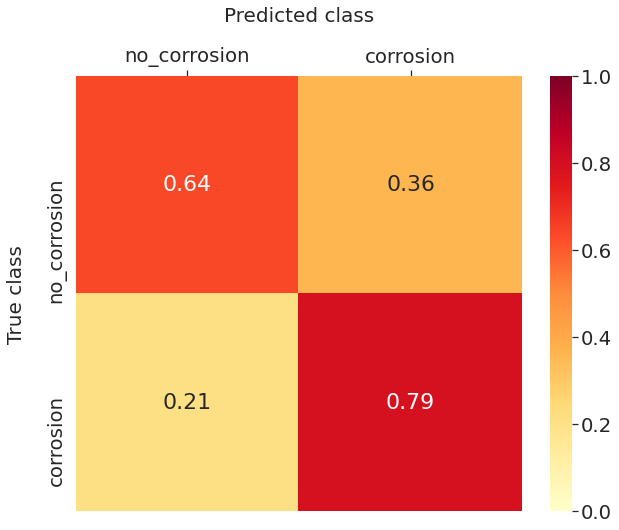
\includegraphics[width=9cm]{images/ResNet_ensemble_3_0,5_average.png} }}%
    \qquad
    \subfloat[\centering Zespół majority]{{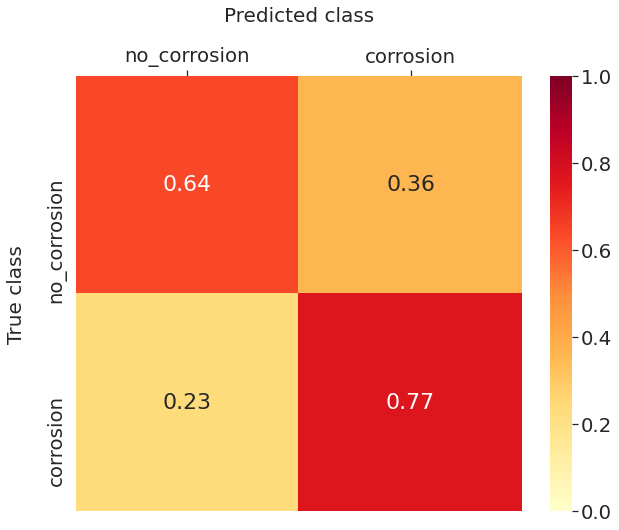
\includegraphics[width=9cm]{images/ResNet_ensemble_3_0,5_majority.png} }}%
    \end{adjustbox}
    \label{fig:resnet-ens-3-0.5-matrices}
    \caption{Tabele \textit{confusion matrix} dla zespołu 3 klasyfikatorów opartych o architekturę ResNet, z parametrem coverage=0.5}
\end{figure}

\noindent Zespół 3 podklasyfikatorów, coverage=0.7:
 \begin{longtable}[h!]{|m{2.6cm}|m{1.2cm}|m{1.2cm}|m{1.2cm}|m{1.2cm}|m{1.2cm}|m{1.2cm}|m{1.2cm}|m{1.2cm}|}
 \hline
 Klasyfikator & Acc & Loss & TP & FP & TN & FN & Prec & Rec\\
 \hline
 Klasyfikator 1 & 0.67 & 0.60 & 655 & 360 & 206 & 63 & 0.64 & 0.91\\
 \hline
 Klasyfikator 2 & 0.61 & 0.64 & 408 & 189 & 377 & 310 & 0.68 & 0.57\\
 \hline
 Klasyfikator 3 & 0.56 & 0.69 & 297 & 133 & 433 & 421 & 0.69 & 0.41\\
 \hline
 Zespół average & 0.67 & 0.60 & 523 & 234 & 332 & 195 & 0.69 & 0.73\\ 
 \hline
 Zespół \newline majority & 0.65 & 1.55 & 490 & 220 & 346 & 228 & 0.69 & 0.68\\
 \hline
\caption{Miary jakości sieci dla klasyfikatorów zespołowych oraz wchodzących w ich skład podklasyfikatorów dla sieci ResNet, zespołu 3 podklasyfikatorów oraz parametru coverage=0.7}
\label{table:19}
\end{longtable}

\noindent Znormalizowane tabele \textit{confusion matrix} dla powyższych klasyfikatorów zespołowych:
\begin{figure}[h!]%
    \begin{adjustbox}{minipage=1.0\paperwidth, pagecenter}
    \centering
    \subfloat[\centering Zespół average]{{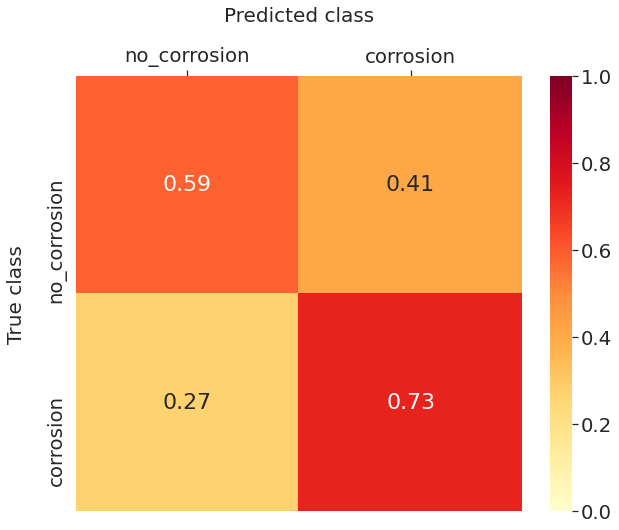
\includegraphics[width=8.7cm]{images/ResNet_ensemble_3_0,7_average.png} }}%
    \qquad
    \subfloat[\centering Zespół majority]{{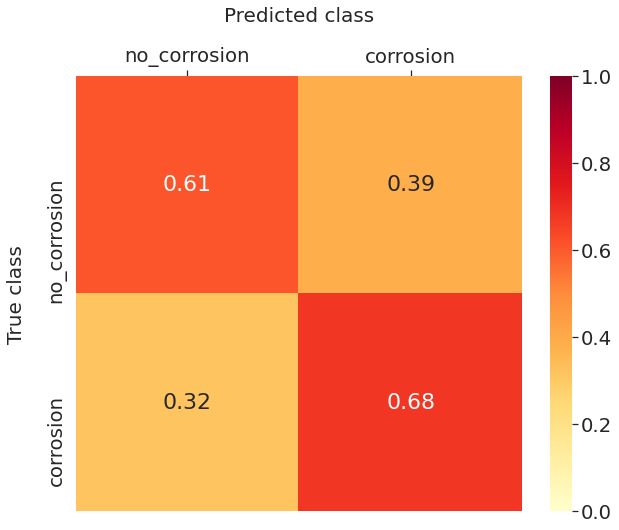
\includegraphics[width=8.7cm]{images/ResNet_ensemble_3_0,7_majority.png} }}%
    \end{adjustbox}
    \label{fig:resnet-ens-3-0.7-matrices}
    \caption{Tabele \textit{confusion matrix} dla zespołu 3 klasyfikatorów opartych o architekturę ResNet, z parametrem coverage=0.7}
\end{figure}

\vspace{3mm}
\noindent Zespół 5 podklasyfikatorów, coverage=None:
 \begin{longtable}[h!]{|m{2.6cm}|m{1.2cm}|m{1.2cm}|m{1.2cm}|m{1.2cm}|m{1.2cm}|m{1.2cm}|m{1.2cm}|m{1.2cm}|}
 \hline
 Klasyfikator & Acc & Loss & TP & FP & TN & FN & Prec & Rec\\
 \hline
 Klasyfikator 1 & 0.68 & 0.58 & 436 & 126 & 440 & 282 & 0.78 & 0.61\\
 \hline
 Klasyfikator 2 & 0.71 & 0.55 & 506 & 155 & 411 & 212 & 0.77 & 0.70\\
 \hline
 Klasyfikator 3 & 0.61 & 0.73 & 533 & 314 & 252 & 185 & 0.63 & 0.74\\
 \hline
 Klasyfikator 4 & 0.61 & 0.78 & 458 & 247 & 319 & 260 & 0.65 & 0.64\\
 \hline
 Klasyfikator 5 & 0.62 & 0.64 & 404 & 171 & 395 & 314 & 0.70 & 0.56\\
 \hline
 Zespół average & 0.71 & 0.57 & 517 & 166 & 400 & 201 & 0.76 & 0.72\\ 
 \hline
 Zespół \newline majority & 0.69 & 1.55 & 494 & 169 & 397 & 224 & 0.75 & 0.69\\
 \hline
\caption{Miary jakości sieci dla klasyfikatorów zespołowych oraz wchodzących w ich skład podklasyfikatorów dla sieci ResNet, zespołu 5 podklasyfikatorów oraz parametru coverage=None}
\label{table:20}
\end{longtable}

\noindent Znormalizowane tabele \textit{confusion matrix} dla powyższych klasyfikatorów zespołowych:
\begin{figure}[h!]%
    \begin{adjustbox}{minipage=1.0\paperwidth, pagecenter}
    \centering
    \subfloat[\centering Zespół average]{{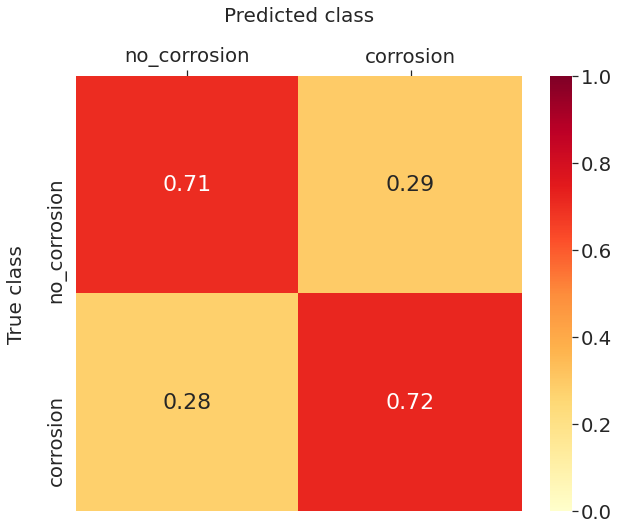
\includegraphics[width=8.7cm]{images/ResNet_ensemble_5_None_average.png} }}%
    \qquad
    \subfloat[\centering Zespół majority]{{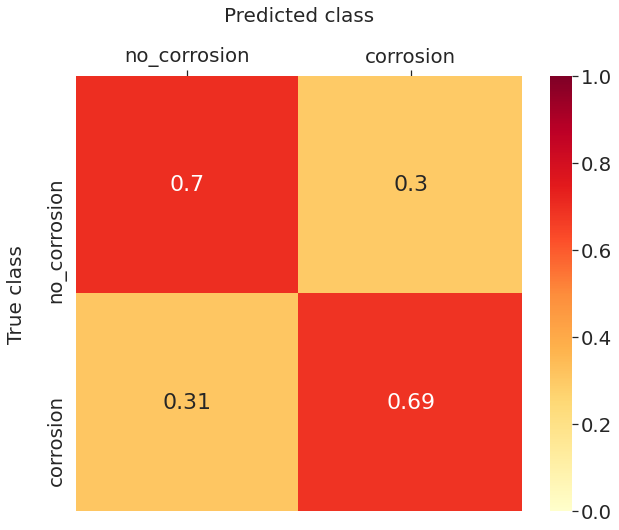
\includegraphics[width=8.7cm]{images/ResNet_ensemble_5_None_majority.png} }}%
    \end{adjustbox}
    \label{fig:resnet-ens-5-None-matrices}
    \caption{Tabele \textit{confusion matrix} dla zespołu 5 klasyfikatorów opartych o architekturę ResNet, z parametrem coverage=None}
\end{figure}

\noindent Zespół 5 podklasyfikatorów, coverage=0.5:
\renewcommand{\arraystretch}{1.75}
 \begin{longtable}[h!]{|m{2.6cm}|m{1.2cm}|m{1.2cm}|m{1.2cm}|m{1.2cm}|m{1.2cm}|m{1.2cm}|m{1.2cm}|m{1.2cm}|}
 \hline
 Klasyfikator & Acc & Loss & TP & FP & TN & FN & Prec & Rec\\
 \hline
 Klasyfikator 1 & 0.71 & 0.57 & 627 & 283 & 283 & 91 & 0.69 & 0.87\\
 \hline
 Klasyfikator 2 & 0.64 & 0.61 & 414 & 157 & 409 & 304 & 0.73 & 0.58\\
 \hline
 Klasyfikator 3 & 0.68 & 0.58 & 390 & 77 & 489 & 328 & 0.84 & 0.54\\
 \hline
 Klasyfikator 4 & 0.68 & 0.63 & 505 & 199 & 367 & 213 & 0.72 & 0.70\\
 \hline
 Klasyfikator 5 & 0.70 & 0.58 & 464 & 132 & 434 & 254 & 0.78 & 0.65\\
 \hline
 Zespół average & 0.73 & 0.54 & 529 & 155 & 411 & 189 & 0.77 & 0.74\\ 
 \hline
 Zespół \newline majority & 0.72 & 1.57 & 475 & 121 & 445 & 243 & 0.80 & 0.66\\
 \hline
\caption{Miary jakości sieci dla klasyfikatorów zespołowych oraz wchodzących w ich skład podklasyfikatorów dla sieci ResNet, zespołu 5 podklasyfikatorów oraz parametru coverage=0.5}
\label{table:21}
\end{longtable}

\noindent Znormalizowane tabele \textit{confusion matrix} dla powyższych klasyfikatorów zespołowych:
\begin{figure}[H]%
    \begin{adjustbox}{minipage=1.0\paperwidth, pagecenter}
    \centering
    \subfloat[\centering Zespół average]{{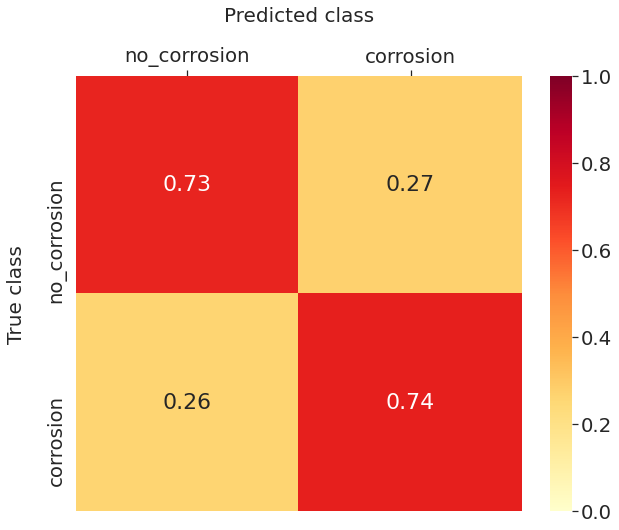
\includegraphics[width=9cm]{images/ResNet_ensemble_5_0,5_average.png} }}%
    \qquad
    \subfloat[\centering Zespół majority]{{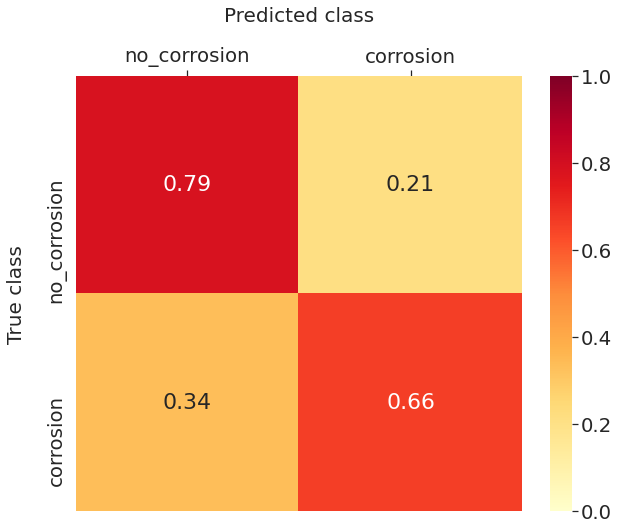
\includegraphics[width=9cm]{images/ResNet_ensemble_5_0,5_majority.png} }}%
    \end{adjustbox}
    \label{fig:resnet-ens-5-0.5-matrices}
    \caption{Tabele \textit{confusion matrix} dla zespołu 5 klasyfikatorów opartych o architekturę ResNet, z parametrem coverage=0.5}
\end{figure}

\vspace{4mm}
\noindent Zespół 5 podklasyfikatorów, coverage=0.7:
\renewcommand{\arraystretch}{1.75}
 \begin{longtable}[h!]{|m{2.6cm}|m{1.2cm}|m{1.2cm}|m{1.2cm}|m{1.2cm}|m{1.2cm}|m{1.2cm}|m{1.2cm}|m{1.2cm}|}
 \hline
 Klasyfikator & Acc & Loss & TP & FP & TN & FN & Prec & Rec\\
 \hline
 Klasyfikator 1 & 0.74 & 0.54 & 522 & 141 & 425 & 196 & 0.79 & 0.73\\
 \hline
 Klasyfikator 2 & 0.71 & 0.64 & 480 & 129 & 437 & 238 & 0.79 & 0.67\\
 \hline
 Klasyfikator 3 & 0.73 & 0.57 & 552 & 185 & 381 & 166 & 0.75 & 0.77\\
 \hline
 Klasyfikator 4 & 0.71 & 0.57 & 634 & 292 & 274 & 84 & 0.68 & 0.88\\
 \hline
 Klasyfikator 5 & 0.68 & 0.58 & 610 & 297 & 269 & 108 & 0.67 & 0.85\\
 \hline
 Zespół average & 0.73 & 0.52 & 561 & 187 & 379 & 157 & 0.75 & 0.78\\ 
 \hline
 Zespół \newline majority & 0.74 & 1.81 & 580 & 192 & 374 & 138 & 0.75 & 0.81\\
 \hline
\caption{Miary jakości sieci dla klasyfikatorów zespołowych oraz wchodzących w ich skład podklasyfikatorów dla sieci ResNet, zespołu 5 podklasyfikatorów oraz parametru coverage=0.7}
\label{table:22}
\end{longtable}

\noindent Znormalizowane tabele \textit{confusion matrix} dla powyższych klasyfikatorów zespołowych:
\begin{figure}[H]%
    \begin{adjustbox}{minipage=1.0\paperwidth, pagecenter}
    \centering
    \subfloat[\centering Zespół average]{{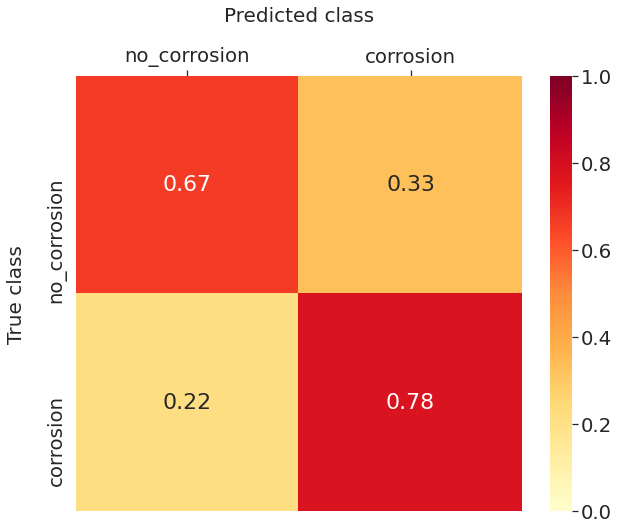
\includegraphics[width=9cm]{images/ResNet_ensemble_5_0,7_average.png} }}%
    \qquad
    \subfloat[\centering Zespół majority]{{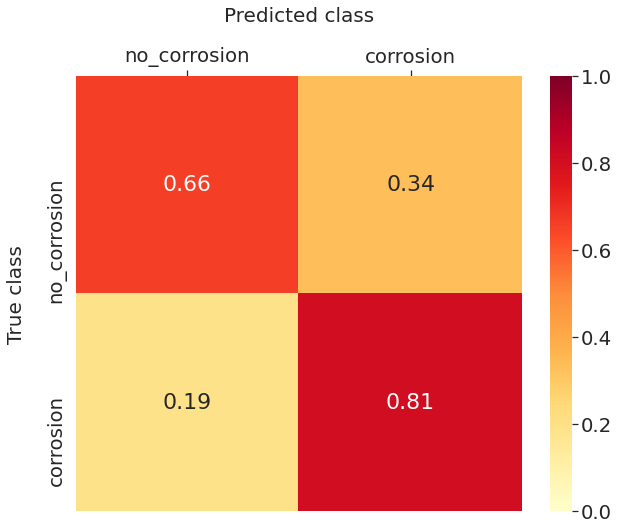
\includegraphics[width=9cm]{images/ResNet_ensemble_5_0,7_majority.png} }}%
    \end{adjustbox}
    \label{fig:resnet-ens-5-0.7-matrices}
    \caption{Tabele \textit{confusion matrix} dla zespołu 5 klasyfikatorów opartych o architekturę ResNet, z parametrem coverage=0.7}
\end{figure}

\vspace{3mm}
\par\noindent Inception:
\vspace{3mm}
\newline\noindent Zespół 3 podklasyfikatorów, coverage=None:
\renewcommand{\arraystretch}{1.55}
 \begin{longtable}[h!]{|m{2.6cm}|m{1.2cm}|m{1.2cm}|m{1.2cm}|m{1.2cm}|m{1.2cm}|m{1.2cm}|m{1.2cm}|m{1.2cm}|}
 \hline
 Klasyfikator & Acc & Loss & TP & FP & TN & FN & Prec & Rec\\
 \hline
 Klasyfikator 1 & 0.71 & 0.57 & 445 & 105 & 461 & 273 & 0.81 & 0.62\\
 \hline
 Klasyfikator 2 & 0.72 & 0.54 & 502 & 142 & 424 & 216 & 0.78 & 0.70\\
 \hline
 Klasyfikator 3 & 0.68 & 0.61 & 627 & 316 & 250 & 91 & 0.66 & 0.87\\
 \hline
 Zespół average & 0.75 & 0.51 & 568 & 166 & 400 & 150 & 0.77 & 0.79\\ 
 \hline
 Zespół \newline majority & 0.74 & 1.60 & 554 & 165 & 401 & 164 & 0.77 & 0.77\\
 \hline
\caption{Miary jakości sieci dla klasyfikatorów zespołowych oraz wchodzących w ich skład podklasyfikatorów dla sieci Inception, zespołu 3 podklasyfikatorów i parametru coverage=None}
\label{table:23}
\end{longtable}

\noindent Znormalizowane tabele \textit{confusion matrix} dla powyższych klasyfikatorów zespołowych:
\begin{figure}[H]%
    \begin{adjustbox}{minipage=1.0\paperwidth, pagecenter}
    \centering
    \subfloat[\centering Zespół average]{{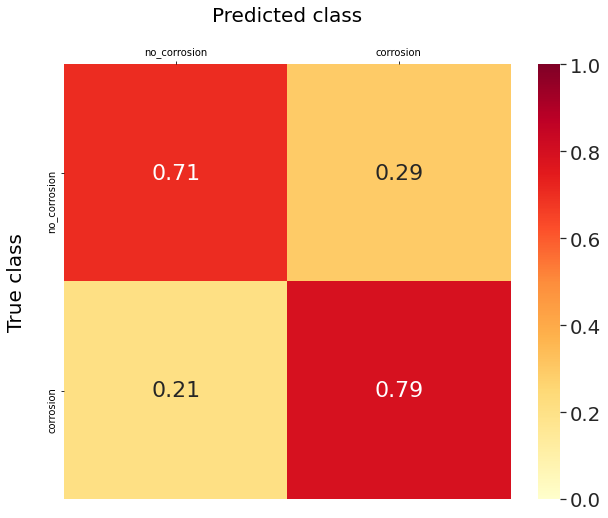
\includegraphics[width=9.2cm]{images/Inception_ensemble_3_None_average.png} }}%
    \qquad
    \subfloat[\centering Zespół majority]{{\includegraphics[width=9.2cm]{images/Inception_ensemble_3_None_majority.png} }}%
    \end{adjustbox}
    \label{fig:inc-ens-3-None-matrices}
    \caption{Tabele \textit{confusion matrix} dla zespołu 3 klasyfikatorów opartych o architekturę Inception, z parametrem coverage=None}
\end{figure}

\noindent Zespół 3 podklasyfikatorów, coverage=0.5:
\renewcommand{\arraystretch}{1.75}
 \begin{longtable}[h!]{|m{2.6cm}|m{1.2cm}|m{1.2cm}|m{1.2cm}|m{1.2cm}|m{1.2cm}|m{1.2cm}|m{1.2cm}|m{1.2cm}|}
 \hline
 Klasyfikator & Acc & Loss & TP & FP & TN & FN & Prec & Rec\\
 \hline
 Klasyfikator 1 & 0.71 & 0.54 & 548 & 199 & 367 & 170 & 0.73 & 0.76\\
 \hline
 Klasyfikator 2 & 0.74 & 0.54 & 527 & 144 & 422 & 191 & 0.79 & 0.73\\
 \hline
 Klasyfikator 3 & 0.69 & 0.59 & 532 & 209 & 357 & 186 & 0.72 & 0.74\\
 \hline
 Zespół average & 0.73 & 0.53 & 536 & 171 & 395 & 182 & 0.76 & 0.75\\ 
 \hline
 Zespół \newline majority & 0.72 & 2.74 & 542 & 178 & 388 & 176 & 0.75 & 0.75\\
 \hline
\caption{Miary jakości sieci dla klasyfikatorów zespołowych oraz wchodzących w ich skład podklasyfikatorów dla sieci Inception, zespołu 3 podklasyfikatorów oraz parametru coverage=0.5}
\label{table:24}
\end{longtable}
\newpage
\noindent Znormalizowane tabele \textit{confusion matrix} dla powyższych klasyfikatorów zespołowych:
\begin{figure}[h!]%
    \begin{adjustbox}{minipage=1.0\paperwidth, pagecenter}
    \centering
    \subfloat[\centering Zespół average]{{\includegraphics[width=9.2cm]{images/Inception_ensemble_3_0,5_average.png} }}%
    \qquad
    \subfloat[\centering Zespół majority]{{\includegraphics[width=9.2cm]{images/Inception_ensemble_3_0,5_majority.png} }}%
    \end{adjustbox}
    \label{fig:inc-ens-3-0.5-matrices}
    \caption{Tabele \textit{confusion matrix} dla zespołu 3 klasyfikatorów opartych o architekturę Inception, z parametrem coverage=0.5}
\end{figure}

\noindent Zespół 3 podklasyfikatorów, coverage=0.7:
\renewcommand{\arraystretch}{1.75}
 \begin{longtable}[h!]{|m{2.6cm}|m{1.2cm}|m{1.2cm}|m{1.2cm}|m{1.2cm}|m{1.2cm}|m{1.2cm}|m{1.2cm}|m{1.2cm}|}
 \hline
 Klasyfikator & Acc & Loss & TP & FP & TN & FN & Prec & Rec\\
 \hline
 Klasyfikator 1 & 0.73 & 0.57 & 598 & 224 & 342 & 120 & 0.73 & 0.83\\
 \hline
 Klasyfikator 2 & 0.72 & 0.63 & 583 & 230 & 336 & 135 & 0.72 & 0.81\\
 \hline
 Klasyfikator 3 & 0.76 & 0.48 & 586 & 172 & 394 & 132 & 0.77 & 0.82\\
 \hline
 Zespół average & 0.74 & 0.50 & 594 & 215 & 351 & 124 & 0.73 & 0.83\\ 
 \hline
 Zespół \newline majority & 0.73 & 2.66 & 587 & 213 & 353 & 131 & 0.73 & 0.82\\
 \hline
\caption{Miary jakości sieci dla klasyfikatorów zespołowych oraz wchodzących w ich skład podklasyfikatorów dla sieci Inception, zespołu 3 podklasyfikatorów oraz parametru coverage=0.7}
\label{table:25}
\end{longtable}
\newpage
\noindent Znormalizowane tabele \textit{confusion matrix} dla powyższych klasyfikatorów zespołowych:
\begin{figure}[H]%
    \begin{adjustbox}{minipage=1.0\paperwidth, pagecenter}
    \centering
    \subfloat[\centering Zespół average]{{\includegraphics[width=9cm]{images/Inception_ensemble_3_0,7_average.png} }}%
    \qquad
    \subfloat[\centering Zespół majority]{{\includegraphics[width=9cm]{images/Inception_ensemble_3_0,7_majority.png} }}%
    \end{adjustbox}
    \label{fig:inc-ens-3-0.7-matrices}
    \caption{Tabele \textit{confusion matrix} dla zespołu 3 klasyfikatorów opartych o architekturę Inception, z parametrem coverage=0.7}
\end{figure}

\vspace{3mm}
\noindent Zespół 5 podklasyfikatorów, coverage=None:
\renewcommand{\arraystretch}{1.75}
 \begin{longtable}[h!]{|m{2.6cm}|m{1.2cm}|m{1.2cm}|m{1.2cm}|m{1.2cm}|m{1.2cm}|m{1.2cm}|m{1.2cm}|m{1.2cm}|}
 \hline
 Klasyfikator & Acc & Loss & TP & FP & TN & FN & Prec & Rec\\
 \hline
 Klasyfikator 1 & 0.72 & 0.57 & 498 & 146 & 420 & 220 & 0.77 & 0.69\\
 \hline
 Klasyfikator 2 & 0.72 & 0.54 & 543 & 179 & 387 & 175 & 0.75 & 0.76\\
 \hline
 Klasyfikator 3 & 0.62 & 0.78 & 492 & 257 & 309 & 226 & 0.66 & 0.69\\
 \hline
 Klasyfikator 4 & 0.69 & 0.57 & 601 & 282 & 284 & 117 & 0.68 & 0.84\\
 \hline
 Klasyfikator 5 & 0.66 & 0.70 & 537 & 255 & 311 & 181 & 0.68 & 0.75\\
 \hline
 Zespół average & 0.72 & 0.54 & 562 & 198 & 368 & 156 & 0.74 & 0.78\\ 
 \hline
 Zespół \newline majority & 0.73 & 1.74 & 568 & 200 & 366 & 150 & 0.74 & 0.79\\
 \hline
\caption{Miary jakości sieci dla klasyfikatorów zespołowych oraz wchodzących w ich skład podklasyfikatorów dla sieci Inception, zespołu 5 podklasyfikatorów oraz parametru coverage=None}
\label{table:26}
\end{longtable}

\newpage
\noindent Znormalizowane tabele \textit{confusion matrix} dla powyższych klasyfikatorów zespołowych:
\begin{figure}[h!]%
    \begin{adjustbox}{minipage=1.0\paperwidth, pagecenter}
    \centering
    \subfloat[\centering Zespół average]{{\includegraphics[width=9cm]{images/Inception_ensemble_5_None_average.png} }}%
    \qquad
    \subfloat[\centering Zespół majority]{{\includegraphics[width=9cm]{images/Inception_ensemble_5_None_majority.png} }}%
    \end{adjustbox}
    \label{fig:inc-ens-5-None-matrices}
    \caption{Tabele \textit{confusion matrix} dla zespołu 5 klasyfikatorów opartych o architekturę Inception, z parametrem coverage=None}
\end{figure}

\vspace{3mm}
\noindent Zespół 5 podklasyfikatorów, coverage=0.5:
\renewcommand{\arraystretch}{1.75}
 \begin{longtable}[h!]{|m{2.6cm}|m{1.2cm}|m{1.2cm}|m{1.2cm}|m{1.2cm}|m{1.2cm}|m{1.2cm}|m{1.2cm}|m{1.2cm}|}
 \hline
 Klasyfikator & Acc & Loss & TP & FP & TN & FN & Prec & Rec\\
 \hline
 Klasyfikator 1 & 0.74 & 0.51 & 556 & 170 & 396 & 162 & 0.77 & 0.77\\
 \hline
 Klasyfikator 2 & 0.71 & 0.53 & 552 & 211 & 355 & 166 & 0.72 & 0.77\\
 \hline
 Klasyfikator 3 & 0.73 & 0.67 & 606 & 229 & 337 & 112 & 0.73 & 0.84\\
 \hline
 Klasyfikator 4 & 0.67 & 0.63 & 562 & 274 & 292 & 156 & 0.67 & 0.78\\
 \hline
 Klasyfikator 5 & 0.66 & 0.66 & 544 & 265 & 301 & 174 & 0.67 & 0.76\\
 \hline
 Zespół average & 0.73 & 0.51 & 600 & 223 & 343 & 118 & 0.73 & 0.84\\ 
 \hline
 Zespół \newline majority & 0.73 & 1.50 & 583 & 207 & 359 & 135 & 0.74 & 0.81\\
 \hline
\caption{Miary jakości sieci dla klasyfikatorów zespołowych oraz wchodzących w ich skład podklasyfikatorów dla sieci Inception, zespołu 5 podklasyfikatorów oraz parametru coverage=0.5}
\label{table:27}
\end{longtable}

\newpage
\noindent Znormalizowane tabele \textit{confusion matrix} dla powyższych klasyfikatorów zespołowych:
\begin{figure}[h!]%
    \begin{adjustbox}{minipage=1.0\paperwidth, pagecenter}
    \centering
    \subfloat[\centering Zespół average]{{\includegraphics[width=9cm]{images/Inception_ensemble_5_0,5_average.png} }}%
    \qquad
    \subfloat[\centering Zespół majority]{{\includegraphics[width=9cm]{images/Inception_ensemble_5_0,5_majority.png} }}%
    \end{adjustbox}
    \label{fig:inc-ens-5-0.5-matrices}
    \caption{Tabele \textit{confusion matrix} dla zespołu 5 klasyfikatorów opartych o architekturę Inception, z parametrem coverage=0.5}
\end{figure}

\vspace{3mm}
\noindent Zespół 5 podklasyfikatorów, coverage=0.7:
\renewcommand{\arraystretch}{1.75}
 \begin{longtable}[h!]{|m{2.6cm}|m{1.2cm}|m{1.2cm}|m{1.2cm}|m{1.2cm}|m{1.2cm}|m{1.2cm}|m{1.2cm}|m{1.2cm}|}
 \hline
 Klasyfikator & Acc & Loss & TP & FP & TN & FN & Prec & Rec\\
 \hline
 Klasyfikator 1 & 0.71 & 0.55 & 523 & 176 & 390 & 195 & 0.75 & 0.73\\
 \hline
 Klasyfikator 2 & 0.75 & 0.51 & 571 & 175 & 391 & 147 & 0.77 & 0.80\\
 \hline
 Klasyfikator 3 & 0.75 & 0.52 & 529 & 136 & 430 & 189 & 0.80 & 0.74\\
 \hline
 Klasyfikator 4 & 0.73 & 0.53 & 581 & 213 & 353 & 137 & 0.73 & 0.81\\
 \hline
 Klasyfikator 5 & 0.72 & 0.55 & 552 & 200 & 366 & 166 & 0.73 & 0.77\\
 \hline
 Zespół average & 0.75 & 0.50 & 572 & 170 & 396 & 146 & 0.77 & 0.80\\ 
 \hline
 Zespół \newline majority & 0.74 & 1.77 & 574 & 185 & 381 & 144 & 0.76 & 0.80\\
 \hline
\caption{Miary jakości sieci dla klasyfikatorów zespołowych oraz wchodzących w ich skład podklasyfikatorów dla sieci Inception, zespołu 5 podklasyfikatorów oraz parametru coverage=0.7}
\label{table:28}
\end{longtable}
\newpage
\noindent Znormalizowane tabele \textit{confusion matrix} dla powyższych klasyfikatorów zespołowych:
\begin{figure}[h!]%
    \begin{adjustbox}{minipage=1.0\paperwidth, pagecenter}
    \centering
    \subfloat[\centering Zespół average]{{\includegraphics[width=9cm]{images/Inception_ensemble_5_0,7_average.png} }}%
    \qquad
    \subfloat[\centering Zespół majority]{{\includegraphics[width=9cm]{images/Inception_ensemble_5_0,7_majority.png} }}%
    \end{adjustbox}
    \label{fig:inc-ens-5-0.7-matrices}
    \caption{Tabele \textit{confusion matrix} dla zespołu 5 klasyfikatorów opartych o architekturę Inception, z parametrem coverage=0.5}
\end{figure}

\vspace{3mm}
\par\noindent EfficientNetB0:
\vspace{3mm}
\newline\noindent Zespół 3 podklasyfikatorów, coverage=None:
\renewcommand{\arraystretch}{1.75}
 \begin{longtable}[h!]{|m{2.6cm}|m{1.2cm}|m{1.2cm}|m{1.2cm}|m{1.2cm}|m{1.2cm}|m{1.2cm}|m{1.2cm}|m{1.2cm}|}
 \hline
 Klasyfikator & Acc & Loss & TP & FP & TN & FN & Prec & Rec\\
 \hline
 Klasyfikator 1 & 0.67 & 0.70 & 500 & 205 & 361 & 218 & 0.71 & 0.70\\
 \hline
 Klasyfikator 2 & 0.67 & 0.60 & 514 & 226 & 340 & 204 & 0.69 & 0.72\\
 \hline
 Klasyfikator 3 & 0.61 & 0.78 & 393 & 178 & 388 & 325 & 0.69 & 0.55\\
 \hline
 Zespół average & 0.69 & 0.57 & 512 & 190 & 376 & 206 & 0.73 & 0.71\\ 
 \hline
 Zespół \newline majority & 0.69 & 2.19 & 514 & 196 & 370 & 204 & 0.72 & 0.72\\
 \hline
\caption{Miary jakości sieci dla klasyfikatorów zespołowych oraz wchodzących w ich skład podklasyfikatorów dla sieci EfficientNetB0, zespołu 3 podklasyfikatorów oraz parametru coverage=None}
\label{table:29}
\end{longtable}

\newpage
\noindent Znormalizowane tabele \textit{confusion matrix} dla powyższych klasyfikatorów zespołowych:
\begin{figure}[h!]%
    \begin{adjustbox}{minipage=1.0\paperwidth, pagecenter}
    \centering
    \subfloat[\centering Zespół average]{{\includegraphics[width=9.2cm]{images/EfficientNetB0_ensemble_3_None_average.png} }}%
    \qquad
    \subfloat[\centering Zespół majority]{{\includegraphics[width=9.2cm]{images/EfficientNetB0_ensemble_3_None_majority.png} }}%
    \end{adjustbox}
    \label{fig:eff-ens-3-None-matrices}
    \caption{Tabele \textit{confusion matrix} dla zespołu 3 klasyfikatorów opartych o architekturę EfficientNetB0, z parametrem coverage=None}
\end{figure}

\vspace{3mm}
\noindent Zespół 3 podklasyfikatorów, coverage=0.5:
\renewcommand{\arraystretch}{1.75}
 \begin{longtable}[h!]{|m{2.6cm}|m{1.2cm}|m{1.2cm}|m{1.2cm}|m{1.2cm}|m{1.2cm}|m{1.2cm}|m{1.2cm}|m{1.2cm}|}
 \hline
 Klasyfikator & Acc & Loss & TP & FP & TN & FN & Prec & Rec\\
 \hline
 Klasyfikator 1 & 0.73 & 0.54 & 519 & 149 & 417 & 199 & 0.78 & 0.72\\
 \hline
 Klasyfikator 2 & 0.71 & 0.55 & 523 & 176 & 390 & 195 & 0.75 & 0.73\\
 \hline
 Klasyfikator 3 & 0.73 & 0.56 & 511 & 140 & 426 & 207 & 0.78 & 0.71\\
 \hline
 Zespół average & 0.75 & 0.51 & 528 & 129 & 437 & 190 & 0.80 & 0.74\\ 
 \hline
 Zespół \newline majority & 0.74 & 2.18 & 527 & 146 & 420 & 191 & 0.78 & 0.73\\
 \hline
\caption{Miary jakości sieci dla klasyfikatorów zespołowych oraz wchodzących w ich skład podklasyfikatorów dla sieci EfficientNetB0, zespołu 3 podklasyfikatorów i parametru coverage=0.5}
\label{table:30}
\end{longtable}

\newpage
\noindent Znormalizowane tabele \textit{confusion matrix} dla powyższych klasyfikatorów zespołowych:
\begin{figure}[h!]%
    \begin{adjustbox}{minipage=1.0\paperwidth, pagecenter}
    \centering
    \subfloat[\centering Zespół average]{{\includegraphics[width=9.2cm]{images/EfficientNetB0_ensemble_3_0,5_average.png} }}%
    \qquad
    \subfloat[\centering Zespół majority]{{\includegraphics[width=9.2cm]{images/EfficientNetB0_ensemble_3_0,5_majority.png} }}%
    \end{adjustbox}
    \label{fig:eff-ens-3-0.5-matrices}
    \caption{Tabele \textit{confusion matrix} dla zespołu 3 klasyfikatorów opartych o architekturę EfficientNetB0, z parametrem coverage=0.5}
\end{figure}

\vspace{3mm}
\noindent Zespół 3 podklasyfikatorów, coverage=0.7:
\renewcommand{\arraystretch}{1.75}
 \begin{longtable}[h!]{|m{2.6cm}|m{1.2cm}|m{1.2cm}|m{1.2cm}|m{1.2cm}|m{1.2cm}|m{1.2cm}|m{1.2cm}|m{1.2cm}|}
 \hline
 Klasyfikator & Acc & Loss & TP & FP & TN & FN & Prec & Rec\\
 \hline
 Klasyfikator 1 & 0.74 & 0.54 & 525 & 147 & 419 & 193 & 0.78 & 0.73\\
 \hline
 Klasyfikator 2 & 0.69 & 0.72 & 505 & 186 & 380 & 213 & 0.73 & 0.70\\
 \hline
 Klasyfikator 3 & 0.76 & 0.50 & 564 & 160 & 406 & 154 & 0.78 & 0.79\\
 \hline
 Zespół average & 0.75 & 0.50 & 535 & 139 & 427 & 183 & 0.79 & 0.75\\ 
 \hline
 Zespół \newline majority & 0.76 & 1.94 & 535 & 137 & 429 & 168 & 0.80 & 0.77\\
 \hline
\caption{Miary jakości sieci dla klasyfikatorów zespołowych oraz wchodzących w ich skład podklasyfikatorów dla sieci EfficientNetB0, zespołu 3 podklasyfikatorów oraz parametru coverage=0.7}
\label{table:31}
\end{longtable}

\newpage
\noindent Znormalizowane tabele \textit{confusion matrix} dla powyższych klasyfikatorów zespołowych:
\begin{figure}[h!]%
    \begin{adjustbox}{minipage=1.0\paperwidth, pagecenter}
    \centering
    \subfloat[\centering Zespół average]{{\includegraphics[width=9.2cm]{images/EfficientNetB0_ensemble_3_0,7_average.png} }}%
    \qquad
    \subfloat[\centering Zespół majority]{{\includegraphics[width=9.2cm]{images/EfficientNetB0_ensemble_3_0,7_majority.png} }}%
    \end{adjustbox}
    \label{fig:eff-ens-3-0.7-matrices}
    \caption{Tabele \textit{confusion matrix} dla zespołu 3 klasyfikatorów opartych o architekturę EfficientNetB0, z parametrem coverage=0.7}
\end{figure}

\vspace{3mm}
\noindent Zespół 5 podklasyfikatorów, coverage=None:
\renewcommand{\arraystretch}{1.75}
 \begin{longtable}[h!]{|m{2.6cm}|m{1.2cm}|m{1.2cm}|m{1.2cm}|m{1.2cm}|m{1.2cm}|m{1.2cm}|m{1.2cm}|m{1.2cm}|}
 \hline
 Klasyfikator & Acc & Loss & TP & FP & TN & FN & Prec & Rec\\
 \hline
 Klasyfikator 1 & 0.69 & 0.91 & 504 & 189 & 377 & 214 & 0.73 & 0.70\\
 \hline
 Klasyfikator 2 & 0.64 & 0.62 & 372 & 111 & 455 & 346 & 0.77 & 0.52\\
 \hline
 Klasyfikator 3 & 0.63 & 0.82 & 444 & 198 & 368 & 274 & 0.69 & 0.62\\
 \hline
 Klasyfikator 4 & 0.66 & 0.68 & 378 & 100 & 466 & 340 & 0.79 & 0.53\\
 \hline
 Klasyfikator 5 & 0.67 & 0.89 & 636 & 340 & 226 & 82 & 0.65 & 0.89\\
 \hline
 Zespół average & 0.70 & 0.56 & 516 & 182 & 384 & 202 & 0.74 & 0.72\\ 
 \hline
 Zespół \newline majority & 0.69 & 1.39 & 499 & 76 & 390 & 219 & 0.74 & 0.69\\
 \hline
\caption{Miary jakości sieci dla klasyfikatorów zespołowych oraz wchodzących w ich skład podklasyfikatorów dla sieci EfficientNetB0, zespołu 5 podklasyfikatorów oraz parametru coverage=None}
\label{table:32}
\end{longtable}

\newpage
\noindent Znormalizowane tabele \textit{confusion matrix} dla powyższych klasyfikatorów zespołowych:
\begin{figure}[h!]%
    \begin{adjustbox}{minipage=1.0\paperwidth, pagecenter}
    \centering
    \subfloat[\centering Zespół average]{{\includegraphics[width=9.2cm]{images/EfficientNetB0_ensemble_5_None_average.png} }}%
    \qquad
    \subfloat[\centering Zespół majority]{{\includegraphics[width=9.2cm]{images/EfficientNetB0_ensemble_5_None_majority.png} }}%
    \end{adjustbox}
    \label{fig:eff-ens-5-None-matrices}
    \caption{Tabele \textit{confusion matrix} dla zespołu 5 klasyfikatorów opartych o architekturę EfficientNetB0, z parametrem coverage=None}
\end{figure}

\vspace{3mm}
\noindent Zespół 5 podklasyfikatorów, coverage=0.5:
\renewcommand{\arraystretch}{1.75}
 \begin{longtable}[h!]{|m{2.6cm}|m{1.2cm}|m{1.2cm}|m{1.2cm}|m{1.2cm}|m{1.2cm}|m{1.2cm}|m{1.2cm}|m{1.2cm}|}
 \hline
 Klasyfikator & Acc & Loss & TP & FP & TN & FN & Prec & Rec\\
 \hline
 Klasyfikator 1 & 0.72 & 0.62 & 443 & 91 & 475 & 275 & 0.83 & 0.62\\
 \hline
 Klasyfikator 2 & 0.70 & 0.54 & 469 & 132 & 434 & 249 & 0.78 & 0.65\\
 \hline
 Klasyfikator 3 & 0.72 & 0.56 & 488 & 126 & 440 & 230 & 0.79 & 0.68\\
 \hline
 Klasyfikator 4 & 0.73 & 0.57 & 490 & 122 & 444 & 228 & 0.80 & 0.68\\
 \hline
 Klasyfikator 5 & 0.70 & 0.57 & 503 & 168 & 398 & 215 & 0.75 & 0.70\\
 \hline
 Zespół average & 0.75 & 0.51 & 491 & 95 & 471 & 227 & 0.84 & 0.68\\ 
 \hline
 Zespół \newline majority & 0.74 & 1.61 & 490 & 106 & 460 & 228 & 0.82 & 0.68\\
 \hline
\caption{Miary jakości sieci dla klasyfikatorów zespołowych oraz wchodzących w ich skład podklasyfikatorów dla sieci EfficientNetB0, zespołu 5 podklasyfikatorów oraz parametru coverage=0.5}
\label{table:33}
\end{longtable}

\newpage
\noindent Znormalizowane tabele \textit{confusion matrix} dla powyższych klasyfikatorów zespołowych:
\begin{figure}[h!]%
    \begin{adjustbox}{minipage=1.0\paperwidth, pagecenter}
    \centering
    \subfloat[\centering Zespół average]{{\includegraphics[width=9.2cm]{images/EfficientNetB0_ensemble_5_0,5_average.png} }}%
    \qquad
    \subfloat[\centering Zespół majority]{{\includegraphics[width=9.2cm]{images/EfficientNetB0_ensemble_5_0,5_majority.png} }}%
    \end{adjustbox}
    \label{fig:eff-ens-5-0.5-matrices}
    \caption{Tabele \textit{confusion matrix} dla zespołu 5 klasyfikatorów opartych o architekturę EfficientNetB0, z parametrem coverage=0.5}
\end{figure}

\vspace{3mm}
\noindent Zespół 5 podklasyfikatorów, coverage=0.7:
\renewcommand{\arraystretch}{1.75}
 \begin{longtable}[h!]{|m{2.6cm}|m{1.2cm}|m{1.2cm}|m{1.2cm}|m{1.2cm}|m{1.2cm}|m{1.2cm}|m{1.2cm}|m{1.2cm}|}
 \hline
 Klasyfikator & Acc & Loss & TP & FP & TN & FN & Prec & Rec\\
 \hline
 Klasyfikator 1 & 0.72 & 0.56 & 536 & 183 & 383 & 182 & 0.75 & 0.75\\
 \hline
 Klasyfikator 2 & 0.73 & 0.54 & 477 & 108 & 458 & 241 & 0.82 & 0.66\\
 \hline
 Klasyfikator 3 & 0.71 & 0.57 & 486 & 137 & 429 & 232 & 0.78 & 0.68\\
 \hline
 Klasyfikator 4 & 0.70 & 0.62 & 520 & 190 & 376 & 198 & 0.73 & 0.72\\
 \hline
 Klasyfikator 5 & 0.76 & 0.50 & 572 & 165 & 401 & 146 & 0.78 & 0.80\\
 \hline
 Zespół average & 0.75 & 0.50 & 537 & 140 & 426 & 181 & 0.79 & 0.75\\ 
 \hline
 Zespół \newline majority & 0.75 & 1.64 & 531 & 128 & 438 & 187 & 0.81 & 0.74\\
 \hline
\caption{Miary jakości sieci dla klasyfikatorów zespołowych oraz wchodzących w ich skład podklasyfikatorów dla sieci EfficientNetB0, zespołu 5 podklasyfikatorów oraz parametru coverage=0.7}
\label{table:34}
\end{longtable}

\newpage
\noindent Znormalizowane tabele \textit{confusion matrix} dla powyższych klasyfikatorów zespołowych:
\begin{figure}[h!]%
    \begin{adjustbox}{minipage=1.0\paperwidth, pagecenter}
    \centering
    \subfloat[\centering Zespół average]{{\includegraphics[width=9.2cm]{images/EfficientNetB0_ensemble_5_0,7_average.png} }}%
    \qquad
    \subfloat[\centering Zespół majority]{{\includegraphics[width=9.2cm]{images/EfficientNetB0_ensemble_5_0,7_majority.png} }}%
    \end{adjustbox}
     \label{fig:eff-ens-5-0.7-matrices}
    \caption{Tabele \textit{confusion matrix} dla zespołu 5 klasyfikatorów opartych o architekturę EfficientNetB0, z parametrem coverage=0.7}
\end{figure}

\par
Wykorzystanie klasyfikatorów zespołowych pozwoliło na osiągnięcie lepszych wyników miar jakości klasyfikacji niż wykorzystanie pojedynczych klasyfikatorów o takich samych architekturach. W zdecydowanej większości przypadków lepsze wyniki pozwoliła uzyskać metoda fuzji decyzji \textit{average voting}. Dla większości klasyfikatorów wyniki lepszego spośród klasyfikatorów zespołowych okazały się być lepsze niż wyniki osiągnięte przez najlepszy spośród klasyfikatorów wchodzących w skład zespołu.
\par
Zespoły klasyfikatorów oparte o architekturę ResNet nie pozwoliły na osiągnięcie wyników wyróżniających się na tle innych klasyfikatorów - najlepsze uzyskane \textit{accuracy} wynosi 74\% (dla zespołu 5 podklasyfikatorów i parametru \textit{coverage}=0.7), jednak wyniki fałszywie pozytywne stanowią w tym przypadku aż 34\% wyników dla klasy o etykietach negatywnych, co eliminuje ten klasyfikator w kontekście dalszych rozważań. Pozostałe zespoły osiągnęły znacząco niższe wyniki w kontekście \textit{accuracy} lub odsetka wyników fałszywych na tle wyników dla danej klasy.
\par
Zespoły klasyfikatorów oparte o architekturę Inception pozwoliły na osiągnięcie lepszej jakości klasyfikacji niż zespoły oparte o architekturę ResNet. Spośród tych klasyfikatorów szczególnie wyróżniają się dwa - zespół złożony z 3 podklasyfikatorów, o parametrze \textit{coverage}=None i metodzie fuzji decyzji \textit{average voting}, który pozwolił na uzyskanie \textit{accuracy} na poziomie 75\% przy wynikach fałszywie negatywnych stanowiących 21\% wyników dla klasy o etykietach pozytywnych (i wynikach fałszywie pozytywnych stanowiących 29\% wyników dla klasy o etykietach negatywnych) oraz zespół złożony z 5 podklasyfikatorów, o parametrze \textit{coverage}=0.7 i metodzie fuzji decyzji \textit{average voting}, który również uzyskał \textit{accuracy} na poziomie 75\% przy wynikach fałszywie negatywnych stanowiących 20\% wyników dla klasy o etykietach pozytywnych (i wynikach fałszywie pozytywnych stanowiących 30\% wyników dla klasy o etykietach negatywnych).
\par
Wśród zespołów klasyfikatorów opartych o architekturę EfficientNetB0 pojawił się zespół, który osiągnął najwyższe \textit{accuracy} spośród wszystkich klasyfikatorów zespołowych - był to klasyfikator złożony z 3 podklasyfikatorów, z parametrem \textit{coverage}=0.7 oraz wykorzystujący \textit{majority voting} - 76\%. Zarówno wyniki fałszywie pozytywne jak i fałszywie negatywne stanowiły 24\% wyników dla klas o etykietach odpowiednio negatywnych i pozytywnych. Wysokie wyniki osiągnął również klasyfikator złożony z 3 podklasyfikatorów z parametrem \textit{coverage}=0.5, wykorzystujący \textit{average voting} - pozwolił na uzyskanie 75\% \textit{accuracy} przy wynikach fałszywie negatywnych stanowiących 26\% wyników dla klasy o etykietach pozytywnych oraz wynikach fałszywie pozytywnych stanowiących 23\% wyników dla klasy negatywnej. Klasyfikatorem wyróżniającym się w klasyfikacji zdjęć należących do klasy negatywnej (i jednocześnie osiągającym jedno z najwyższych \textit{accuracy}, tzn. na poziomie 75\%) był klasyfikator złożony z 5 podklasyfikatorów, o parametrze \textit{coverage}=0.5 i metodzie fuzji decyzji \textit{average voting} - niepoprawnie sklasyfikował 17\% zdjęć należących do klasy negatywnej (oraz 32\% zdjęć należących do klasy pozytywnej). Warto również przyjrzeć się wynikom klasyfikatorów złożonych z 5 podklasyfikatorów, o parametrze \textit{coverage}=0.7 - zarówno klasyfikator wykorzystujący \textit{average voting} jak i ten wykorzystujący \textit{majority voting} osiągnął \textit{accuracy} na poziomie 75\%, przy niepoprawnej klasyfikacji 25\% zdjęć z klasy negatywnej i 25\% z klasy pozytywnej przez pierwszy oraz niepoprawnej klasyfikacji 23\% zdjęć z klasy negatywnej i 26\% zdjęć z klasy pozytywnej przez drugi zespół.
\par
Uzyskane wyniki są lepsze niż wyniki osiągnięte przez pojedyncze klasyfikatory o tych samych architekturach, jednak liczby wyników fałszywie negatywnych są zbyt wysokie w kontekście wykorzystania tych sieci w końcowym produkcie. Wyróżnione zostały klasyfikatory osiągające zarówno odznaczające się wyniki klasyfikacji klasy pozytywnej jak i negatywnej (przy jednocześnie osiągniętym wysokim \textit{accuracy}), w celu ich dalszej analizy pod kątem manipulacji progiem przynależności zdjęć do klasy pozytywnej w celu zmniejszenia liczby wyników fałszywie negatywnych.


\subsubsection{Manipulacja progiem przydzielania zdjęć dla klasyfikatorów zespołowych}

\par Klasyfikatory zespołowe osiągające najlepsze wyniki miar jakości klasyfikacji poddano próbie dostosowania progu przydzielania zdjęć do klasy pozytywnej dla zmniejszenia liczby wyników fałszywie negatywnych. Ponownie wykorzystano progi: 0.5, 0.45, 0.4, 0.35, 0.3 i 0.25.
\vspace{3mm}
\newline Wyniki eksperymentu przedstawiono poniżej:
\vspace{3mm}

\par\noindent Sieć Inception, 3 podklasyfikatory, coverage=None, average voting:
\renewcommand{\arraystretch}{1.65}
 \begin{longtable}[h!]{|m{2.0cm}|m{1.2cm}|m{1.2cm}|m{1.2cm}|m{1.2cm}|m{1.2cm}|m{1.2cm}|m{1.2cm}|m{1.6cm}|}
 \hline
 Próg & Acc & TP & FP & TN & FN & Prec & Rec & F1 score\\
 \hline
 0.5 & 0.75 & 568 & 166 & 400 & 150 & 0.77 & 0.79 & 0.78\\
 \hline
 0.45 & 0.74 & 611 & 224 & 342 & 107 & 0.73 & 0.85 & 0.79\\
 \hline
 0.4 & 0.72 & 651 & 292 & 274 & 67 & 0.69 & 0.91 & 0.78\\
 \hline
 0.35 & 0.69 & 679 & 354 & 212 & 39 & 0.66 & 0.95 & 0.78\\
 \hline
 0.3 & 0.66 & 697 & 418 & 148 & 21 & 0.63 & 0.97 & 0.76\\
 \hline
 0.25 & 0.62 & 713 & 488 & 78 & 5 & 0.59 & 0.99 & 0.74\\
 \hline
\caption{Miary jakości klasyfikatora zespołowego opartego o architekturę Inception, złożonego z 3 podklasyfikatorów z parametrem coverage=None i metodą fuzji decyzji average voting dla różnych progów dla klasy pozytywnej}
\label{table:35}
\end{longtable}

\begin{figure}[H]
    \begin{adjustbox}{minipage=1.0\paperwidth, pagecenter}
    \centering
    \subfloat[\centering Confusion matrix dla domyślnego progu - 0.5]{{\includegraphics[width=8.7cm]{images/Inc_ensemble_3_None_avg_0,5.png} }}%
    \qquad
    \subfloat[\centering Confusion matrix dla najlepszego progu - 0.4]{{\includegraphics[width=8.7cm]{images/Inc_ensemble_3_None_avg_0,4.png} }}%
    \end{adjustbox}
    \label{fig:inc-ens-3-None-avg-thresh-matrices}
    \caption{Tabele \textit{confusion matrix} dla zespołu 3 klasyfikatorów opartych o architekturę Inception, z parametrem coverage=None i metodą fuzji decyzji average voting dla progów domyślnego i najlepszego}
\end{figure}

\par\noindent Sieć Inception, 5 podklasyfikatorów, coverage=0.7, average voting:
\renewcommand{\arraystretch}{1.57}
 \begin{longtable}[h!]{|m{2.0cm}|m{1.2cm}|m{1.2cm}|m{1.2cm}|m{1.2cm}|m{1.2cm}|m{1.2cm}|m{1.2cm}|m{1.6cm}|}
 \hline
 Próg & Acc & TP & FP & TN & FN & Prec & Rec & F1 score\\
 \hline
 0.5 & 0.75 & 572 & 170 & 396 & 146 & 0.77 & 0.80 & 0.78\\
 \hline
 0.45 & 0.74 & 594 & 215 & 351 & 124 & 0.73 & 0.83 & 0.78\\
 \hline
 0.4 & 0.72 & 624 & 260 & 306 & 94 & 0.71 & 0.87 & 0.78\\
 \hline
 0.35 & 0.71 & 650 & 298 & 268 & 68 & 0.69 & 0.91 & 0.78\\
 \hline
 0.3 & 0.70 & 673 & 345 & 221 & 45 & 0.66 & 0.94 & 0.78\\
 \hline
 0.25 & 0.67 & 695 & 406 & 160 & 23 & 0.63 & 0.97 & 0.76\\
 \hline
\caption{Miary jakości klasyfikatora zespołowego opartego o architekturę Inception, złożonego z 5 podklasyfikatorów z parametrem coverage=0.7 i metodą fuzji decyzji average voting dla różnych progów dla klasy pozytywnej}
\label{table:36}
\end{longtable}

\begin{figure}[H]
    \begin{adjustbox}{minipage=1.0\paperwidth, pagecenter}
    \centering
    \subfloat[\centering Confusion matrix dla domyślnego progu - 0.5]{{\includegraphics[width=9cm]{images/Inc_ensemble_5_0,7_avg_0,5.png} }}%
    \qquad
    \subfloat[\centering Confusion matrix dla najlepszego progu - 0.35]{{\includegraphics[width=9cm]{images/Inc_ensemble_5_0,7_avg_0,35.png} }}%
    \end{adjustbox}
    \label{fig:inc-ens-5-0.7-avg-thresh-matrices}
    \caption{Tabele \textit{confusion matrix} dla zespołu 5 klasyfikatorów opartych o architekturę Inception, z parametrem coverage=0.7 i metodą fuzji decyzji average voting dla progów domyślnego i najlepszego}
\end{figure}

\vspace{3.5mm}
\par\noindent Sieć EfficientNetB0, 3 podklasyfikatory, coverage=0.5, average voting:
\renewcommand{\arraystretch}{1.7}
 \begin{longtable}[h!]{|m{2.0cm}|m{1.2cm}|m{1.2cm}|m{1.2cm}|m{1.2cm}|m{1.2cm}|m{1.2cm}|m{1.2cm}|m{1.6cm}|}
 \hline
 Próg & Acc & TP & FP & TN & FN & Prec & Rec & F1 score\\
 \hline
 0.5 & 0.75 & 528 & 129 & 437 & 190 & 0.80 & 0.74 & 0.77\\
 \hline
 0.45 & 0.75 & 568 & 173 & 393 & 150 & 0.77 & 0.79 & 0.78\\
 \hline
 0.4 & 0.74 & 600 & 222 & 344 & 118 & 0.73 & 0.84 & 0.78\\
 \hline
 0.35 & 0.71 & 631 & 280 & 286 & 87 & 0.69 & 0.88 & 0.77\\
 \hline
 0.3 & 0.69 & 662 & 337 & 229 & 56 & 0.66 & 0.92 & 0.77\\
 \hline
 0.25 & 0.66 & 689 & 407 & 159 & 29 & 0.63 & 0.96 & 0.76\\
 \hline
\caption{Miary jakości klasyfikatora zespołowego opartego o architekturę EfficientNetB0, złożonego z 3 podklasyfikatorów z parametrem coverage=0.5 i metodą fuzji decyzji average voting dla różnych progów dla klasy pozytywnej}
\label{table:37}
\end{longtable}

\begin{figure}[H]
    \begin{adjustbox}{minipage=1.0\paperwidth, pagecenter}
    \centering
    \subfloat[\centering Confusion matrix dla domyślnego progu - 0.5]{{\includegraphics[width=9cm]{images/EffB0_ensemble_3_0,5_avg_0,5.png} }}%
    \qquad
    \subfloat[\centering Confusion matrix dla najlepszego progu - 0.4]{{\includegraphics[width=9cm]{images/EffB0_ensemble_3_0,5_avg_0,4.png} }}%
    \end{adjustbox}
    \label{fig:eff-ens-3-0.5-avg-thresh-matrices}
    \caption{Tabele \textit{confusion matrix} dla zespołu 3 klasyfikatorów opartych o architekturę EfficientNetB0, z parametrem coverage=0.5 i metodą fuzji decyzji average voting dla progów domyślnego i najlepszego}
\end{figure}

\vspace{3.5mm}
\par\noindent Sieć EfficientNetB0, 3 podklasyfikatory, coverage=0.7, majority voting:
 \begin{longtable}[h!]{|m{2.0cm}|m{1.2cm}|m{1.2cm}|m{1.2cm}|m{1.2cm}|m{1.2cm}|m{1.2cm}|m{1.2cm}|m{1.6cm}|}
 \hline
 Próg & Acc & TP & FP & TN & FN & Prec & Rec & F1 score\\
 \hline
 0.5 & 0.76 & 550 & 137 & 429 & 168 & 0.80 & 0.77 & 0.78\\
 \hline
 0.45 & 0.76 & 550 & 137 & 429 & 168 & 0.80 & 0.77 & 0.78\\
 \hline
 0.4 & 0.76 & 550 & 137 & 429 & 168 & 0.80 & 0.77 & 0.78\\
 \hline
 0.35 & 0.76 & 550 & 137 & 429 & 168 & 0.80 & 0.77 & 0.78\\
 \hline
 0.3 & 0.70 & 635 & 304 & 262 & 83 & 0.68 & 0.88 & 0.77\\
 \hline
 0.25 & 0.70 & 635 & 304 & 262 & 83 & 0.68 & 0.88 & 0.77\\
 \hline
\caption{Miary jakości klasyfikatora zespołowego opartego o architekturę EfficientNetB0, złożonego z 3 podklasyfikatorów z parametrem coverage=0.7 i metodą fuzji decyzji majority voting dla różnych progów dla klasy pozytywnej}
\label{table:38}
\end{longtable}

\begin{figure}[H]
    \begin{adjustbox}{minipage=1.0\paperwidth, pagecenter}
    \centering
    \subfloat[\centering Confusion matrix dla domyślnego progu - 0.5]{{\includegraphics[width=9cm]{images/EffB0_3_0,7_mjr_0,5.png} }}%
    \qquad
    \subfloat[\centering Confusion matrix dla progu 0.3]{{\includegraphics[width=9cm]{images/EffB0_3_0,7_mjr_0,3.png} }}%
    \end{adjustbox}
    \label{fig:eff-ens-3-0.7-maj-thresh-matrices}
    \caption{Tabele \textit{confusion matrix} dla zespołu 3 klasyfikatorów opartych o architekturę EfficientNetB0, z parametrem coverage=0.7 i metodą fuzji decyzji majority voting dla progów domyślnego i najlepszego}
\end{figure}

\vspace{3.5mm}
\par\noindent Sieć EfficientNetB0, 5 podklasyfikatorów, coverage=0.5, average voting:
 \begin{longtable}[h!]{|m{2.0cm}|m{1.2cm}|m{1.2cm}|m{1.2cm}|m{1.2cm}|m{1.2cm}|m{1.2cm}|m{1.2cm}|m{1.6cm}|}
 \hline
 Próg & Acc & TP & FP & TN & FN & Prec & Rec & F1 score\\
 \hline
 0.5 & 0.75 & 491 & 95 & 471 & 227 & 0.84 & 0.68 & 0.75\\
 \hline
 0.45 & 0.75 & 527 & 129 & 437 & 191 & 0.80 & 0.73 & 0.77\\
 \hline
 0.4 & 0.75 & 566 & 168 & 398 & 152 & 0.77 & 0.79 & 0.78\\
 \hline
 0.35 & 0.74 & 597 & 216 & 350 & 121 & 0.73 & 0.83 & 0.78\\
 \hline
 0.3 & 0.72 & 627 & 272 & 294 & 91 & 0.70 & 0.87 & 0.78\\
 \hline
 0.25 & 0.69 & 653 & 329 & 237 & 65 & 0.66 & 0.91 & 0.77\\
 \hline
\caption{Miary jakości klasyfikatora zespołowego opartego o architekturę EfficientNetB0, złożonego z 5 podklasyfikatorów z parametrem coverage=0.5 i metodą fuzji decyzji average voting dla różnych progów dla klasy pozytywnej}
\label{table:39}
\end{longtable}

\begin{figure}[H]
    \begin{adjustbox}{minipage=1.0\paperwidth, pagecenter}
    \centering
    \subfloat[\centering Confusion matrix dla domyślnego progu - 0.5]{{\includegraphics[width=9cm]{images/EffB0_ensemble_5_0,5_avg_0,5.png} }}%
    \qquad
    \subfloat[\centering Confusion matrix dla najlepszego progu - 0.35]{{\includegraphics[width=9cm]{images/EffB0_ensemble_5_0,5_avg_0,35.png} }}%
    \end{adjustbox}
    \label{fig:eff-ens-5-0.5-avg-thresh-matrices}
    \caption{Tabele \textit{confusion matrix} dla zespołu 5 klasyfikatorów opartych o architekturę EfficientNetB0, z parametrem coverage=0.5 i metodą fuzji decyzji average voting dla progów domyślnego i najlepszego}
\end{figure}

\vspace{3.5mm}
\par\noindent Sieć EfficientNetB0, 5 podklasyfikatorów, coverage=0.7, average voting:
 \begin{longtable}[h!]{|m{2.0cm}|m{1.2cm}|m{1.2cm}|m{1.2cm}|m{1.2cm}|m{1.2cm}|m{1.2cm}|m{1.2cm}|m{1.6cm}|}
 \hline
 Próg & Acc & TP & FP & TN & FN & Prec & Rec & F1 score\\
 \hline
 0.5 & 0.75 & 537 & 140 & 426 & 181 & 0.79 & 0.75 & 0.77\\
 \hline
 0.45 & 0.74 & 560 & 171 & 395 & 158 & 0.77 & 0.78 & 0.77\\
 \hline
 0.4 & 0.73 & 590 & 221 & 345 & 128 & 0.73 & 0.82 & 0.77\\
 \hline
 0.35 & 0.73 & 622 & 255 & 311 & 96 & 0.71 & 0.87 & 0.78\\
 \hline
 0.3 & 0.70 & 651 & 316 & 250 & 67 & 0.67 & 0.91 & 0.77\\
 \hline
 0.25 & 0.68 & 673 & 362 & 204 & 45 & 0.65 & 0.94 & 0.77\\
 \hline
\caption{Miary jakości klasyfikatora zespołowego opartego o architekturę EfficientNetB0, złożonego z 5 podklasyfikatorów z parametrem coverage=0.7 i metodą fuzji decyzji average voting dla różnych progów dla klasy pozytywnej}
\label{table:40}
\end{longtable}

\begin{figure}[H]
    \begin{adjustbox}{minipage=1.0\paperwidth, pagecenter}
    \centering
    \subfloat[\centering Confusion matrix dla domyślnego progu - 0.5]{{\includegraphics[width=9cm]{images/EffB0_ensemble_5_0,7_avg_0,5.png} }}%
    \qquad
    \subfloat[\centering Confusion matrix dla najlepszego progu - 0.35]{{\includegraphics[width=9cm]{images/EffB0_ensemble_5_0,7_avg_0,35.png} }}%
    \end{adjustbox}
    \label{fig:eff-ens-5-0.7-avg-thresh-matrices}
    \caption{Tabele \textit{confusion matrix} dla zespołu 5 klasyfikatorów opartych o architekturę EfficientNetB0, z parametrem coverage=0.7 i metodą fuzji decyzji average voting dla progów domyślnego i najlepszego}
\end{figure}

\vspace{3.5mm}
\par\noindent Sieć EfficientNetB0, 5 podklasyfikatorów, coverage=0.7, majority voting:
 \begin{longtable}[h!]{|m{2.0cm}|m{1.2cm}|m{1.2cm}|m{1.2cm}|m{1.2cm}|m{1.2cm}|m{1.2cm}|m{1.2cm}|m{1.6cm}|}
 \hline
 Próg & Acc & TP & FP & TN & FN & Prec & Rec & F1 score\\
 \hline
 0.5 & 0.75 & 531 & 128 & 438 & 187 & 0.81 & 0.74 & 0.77\\
 \hline
 0.45 & 0.75 & 531 & 128 & 438 & 187 & 0.81 & 0.74 & 0.77\\
 \hline
 0.4 & 0.75 & 531 & 128 & 438 & 187 & 0.81 & 0.74 & 0.77\\
 \hline
 0.35 & 0.72 & 579 & 219 & 347 & 139 & 0.73 & 0.81 & 0.76\\
 \hline
 0.3 & 0.72 & 579 & 219 & 347 & 139 & 0.73 & 0.81 & 0.76\\
 \hline
 0.25 & 0.72 & 579 & 219 & 347 & 139 & 0.73 & 0.81 & 0.76\\
 \hline
\caption{Miary jakości klasyfikatora zespołowego opartego o architekturę EfficientNetB0, złożonego z 5 podklasyfikatorów z parametrem coverage=0.7 i metodą fuzji decyzji majority voting dla różnych progów dla klasy pozytywnej}
\label{table:41}
\end{longtable}

\begin{figure}[H]
    \begin{adjustbox}{minipage=1.0\paperwidth, pagecenter}
    \centering
    \subfloat[\centering Confusion matrix dla domyślnego progu - 0.5]{{\includegraphics[width=9cm]{images/EffB0_5_0,7_mjr_0,5.png} }}%
    \qquad
    \subfloat[\centering Confusion matrix dla progu 0.35]{{\includegraphics[width=9cm]{images/EffB0_5_0,7_mjr_0,35.png} }}%
    \end{adjustbox}
    \label{fig:eff-ens-5-0.7-maj-thresh-matrices}
    \caption{Tabele \textit{confusion matrix} dla zespołu 5 klasyfikatorów opartych o architekturę EfficientNetB0, z parametrem coverage=0.7 i metodą fuzji decyzji majority voting dla progów domyślnego i najlepszego}
\end{figure}

Dla sieci Inception zbadano wpływ zmiany progu dla dwóch wariantów klasyfikatora grupowego: z 3 podklasyfikatorami, parametrem \textit{coverage}=None i metodą głosowania \textit{average voting} oraz z 5 podklasyfikatorami, parametrem \textit{coverage}=0.7 i metodą głosowania \textit{average voting}. Wyniki \textit{precision} i \textit{recall} dla obu przypadków dla poszczególnych progów były podobne, natomiast \textit{accuracy} dla pierwszego z nich dla coraz niższych progów spadało gwałtowniej. W związku z powyższym najlepszą opcją był wysoki próg 0.4, mimo, że dla niższych progów \textit{recall} osiągał wartości większe lub równe 95\% - w tych przypadkach to \textit{precision} i \textit{accuracy} były nie do przyjęcia. 

Pozostałe klasyfikatory wykorzystywały sieć EfficientNetB0. Dla klasyfikatorów, w których stosowaną metodą fuzji decyzji był \textit{majority voting} i oba miały parametr \textit{coverage}=0.7, a różniły się liczbą podklasyfikatorów (3 i 5), zmiana miar jakości była gwałtowna i następowała dopiero przy niskich progach 0.3 oraz 0.35. Wynika z tego, że klasyfikatory jednoznacznie wskazywały klasę, a lekka manipulacja progiem nie powodowała zmiany ich decyzji. W wersji z 3 podklasyfikatorami przy niskich progach \textit{accuracy} spadło z 76\% do 70\%, natomiast \textit{precision} i \textit{recall} wyniosły odpowiednio 68\% oraz 88\%. Dla 5 podklasyfikatorów \textit{accuracy} spadło z z 75\% do 72\%, \textit{recall} wyniósł 81\%, a \textit{precision} 73\%. Wprowadzenie większej liczby podklasyfikatorów spowodowało, że manipulacja nie wpłynęła tak znacząco na \textit{recall}. 

Podobne porównanie można przeprowadzić z klasyfikatorami z pokryciem \textit{coverage}=0.5 i głosowaniem \textit{average voting} różniącymi się liczbą podklasyfikatorów (3 i 5). Dla wersji z 3 podklasyfikatorami najlepszy próg wyniósł 0.4, a dla 5 podklasyfikatorów 0.35. \textit{Accuracy} (74\%), \textit{precision} (73\%) oraz \textit{F1 Score} (78\%) były identyczne, jednak \textit{recall}, a w konsekwencji mniejsza liczba \textit{false negativów}, był wyższy o 1 p.p. dla wersji z 3 podklasyfikatorami i wyniósł 84\%. Wynika z tego, że liczba podklasyfikatorów niemal wcale nie wpłynęła na wynik manipulacji dla najlepszych progów.

Dla sieci z 5 podklasyfikatorami i parametrem \textit{coverage}=0.7 obie wersje podejmowania decyzji (\textit{average voting} oraz \textit{majority voting}) uzyskały najlepsze wyniki dla progu 0.35. \textit{Accuracy} dla obu przypadków było zbliżone, jednak w wariancie z głosowaniem \textit{average voting} \textit{recall} wyniósł 87\% przy \textit{precision} 71\%, gdy dla \textit{majority voting} \textit{precision} osiągnęło podobną wartość 73\%, ale \textit{recall} miał wartość jedynie 81\%. Klasyfikatory z opcją \textit{average voting} były bardziej podatne na manipulację progiem i dawały możliwość bardziej znaczącego obniżenia liczby \textit{false negativów}.

Najlepsze wyniki uzyskano dla klasyfikatorów opartych o architekturę EfficientNetB0, z parametrem \textit{coverage}=0.5 i metodą głosowania \textit{average voting}. Wersja z 3 podklasyfikatorami dla progu równego 0.4 poprawnie wykrywała skorodowane obiekty ze skutecznością wynoszącą 84\%, a struktury bez korozji z 61\%. Dla 5 podklasyfikatorów i progu 0.35 skuteczność we wskazywaniu korozji zgodnie z prawdą wyniosła 83\%, a jej braku 62\%. Manipulacja progiem w obu przypadkach spowodowała zmniejszenie liczby \textit{false negativów} przy równoczesnym zachowaniu akceptowalnego stopnia rozpoznawania obiektów, które nie były objęte korozją. 

\subsubsection{Treningi z wykorzystaniem standaryzacji danych}
\par
W poprzednich doświadczeniach wykorzystano normalizację danych, tzn. wartości pikseli zostały podzielone przez 255, co w efekcie zmieniło zakres ich wartości z [0;255] do [0;1]. Bardziej rozszerzonym podejściem do wstępnej obróbki danych jest ich standaryzacja, polegająca na takim przekształceniu, w wyniku którego uzyskują one rozkład normalny, a więc z wartością oczekiwaną równą 0 i odchyleniem standardowym 1. Standaryzacja może dotyczyć zarówno całego zbioru danych razem (biorąc pod uwagę statystyki dotyczące całego zbioru) jak i każdego elementu zbioru z osobna (w tym przypadku biorąc pod uwagę statystyki każdego zdjęcia). W pracy zostało zbadane w jaki sposób standaryzacja całego zbioru danych wpływa na jakość klasyfikacji. Operacja ta została przeprowadzona poprzez odjęcie od każdego piksela każdego zdjęcia w zbiorze danych średniej wartości piksela ze zbioru treningowego oraz podzielenie otrzymanych wartości przez odchylenie standardowe wartości pikseli w tym zbiorze.
\par Dodatkowo zastosowaną modyfikacją jest wykorzystanie warstwy GlobalAveragePooling zamiast GlobalMaxPooling - zbadano, że samo wykorzystanie standaryzacji poprawia jakość klasyfikacji, a podmiana rodzaju warstwy GlobalPooling dodatkowo nieco poprawia krzywe uczenia. W pracy zamieszczono ostateczne wyniki uzyskane przy wykorzystaniu standaryzacji danych oraz zastosowaniu warstwy GAP.
\vspace{2mm}
\par\noindent Poniżej przedstawiono wyniki tego eksperymentu:
\renewcommand{\arraystretch}{1.67}
 \begin{longtable}[h!]{|m{2.6cm}|m{1.2cm}|m{1.2cm}|m{1.2cm}|m{1.2cm}|m{1.2cm}|m{1.2cm}|m{1.2cm}|m{1.2cm}|}
 \hline
 Sieć & Acc & Loss & TP & FP & TN & FN & Prec & Rec\\
 \hline
 ResNet & 0.75 & 0.61 & 505 & 103 & 463 & 213 & 0.83 & 0.70\\
 \hline
 Inception & 0.75 & 0.52 & 537 & 144 & 422 & 181 & 0.79 & 0.75\\
 \hline
 EfficientNetB0 & 0.76 & 0.48 & 554 & 150 & 416 & 164 & 0.79 & 0.77\\
 \hline
\caption{Miary jakości dla poszczególnych rodzajów sieci trenowanych na danych poddanych standaryzacji}
\label{table:42}
\end{longtable}

\begin{figure}[H]%
    \begin{adjustbox}{minipage=1.0\paperwidth, pagecenter}
    \centering
    \subfloat[\centering ResNet]{{\includegraphics[width=8.5cm]{images/ResNetStandardize.png} }}%
    \qquad
    \subfloat[\centering Inception]{{\includegraphics[width=8.5cm]{images/InceptionStandardize.png} }}%
    \end{adjustbox}
\end{figure}
\begin{figure}[h!]%
    \ContinuedFloat
    \begin{adjustbox}{minipage=1.0\paperwidth, pagecenter}
    \centering
    \subfloat[\centering EfficientNetB0]{{\includegraphics[width=8.5cm]{images/EfficientNetB0Standardize.png} }}%
    \end{adjustbox}
    \label{fig:std-matrices}
    \caption{Tabele \textit{confusion matrix} dla poszczególnych rodzajów sieci trenowanych na danych poddanych standaryzacji}
\end{figure}

Wszystkie wytrenowane sieci odznaczają się jednymi z najwyższych jakości klasyfikacji (\textit{accuracy} na poziomie 75-76\%). Sieć ResNet osiągnęła najwyższe \textit{precision} - 83\%, a także szczególnie dobrze radzi sobie z klasyfikacją klasy negatywnej - poprawnie klasyfikuje 82\% zdjęć należących do tej klasy. Sieć Inception odznacza się tak samo dobrymi poziomami klasyfikacji klasy pozytywnej i negatywnej - wyniki poprawne stanowią po 75\% wyników w każdej klasie. Sieć EfficientNetB0 osiągnęła najwyższe \textit{accuracy} - 76\% oraz wysokie \textit{precision} i \textit{recall}. Dobrze radzi sobie z klasyfikacją zdjęć z obu klas - poprawnie sklasyfikowała 73\% zdjęć z klasy negatywnej i 77\% zdjęć z klasy pozytywnej.
\par Podobnie jak w poprzednich eksperymentach, sieci zostały dalej poddane próbie dopasowania odpowiedniego progu powyżej którego zdjęcia były klasyfikowane jako skorodowane w celu zmniejszenia liczby wyników fałszywie negatywnych.


\subsubsection{Manipulacja progiem przydzielania zdjęć dla modeli wykorzystujących standaryzację}

\par W celu zmniejszenia liczby wyników fałszywie negatywnych podjęto próbę dostosowania progu przydzielania zdjęć do klasy pozytywnej dla modeli wykorzystujących standaryzację danych. 
\vspace{3mm}
\par\noindent Poniżej znajdują się wyniki tego eksperymentu:
\vspace{3mm}
\par\noindent ResNet:
\renewcommand{\arraystretch}{1.7}
 \begin{longtable}[h!]{|m{2.0cm}|m{1.2cm}|m{1.2cm}|m{1.2cm}|m{1.2cm}|m{1.2cm}|m{1.2cm}|m{1.2cm}|m{1.6cm}|}
 \hline
 Próg & Acc & TP & FP & TN & FN & Prec & Rec & F1 score\\
 \hline
 0.5 & 0.75 & 507 & 105 & 461 & 211 & 0.83 & 0.71 & 0.76\\
 \hline
 0.45 & 0.76 & 522 & 115 & 451 & 196 & 0.82 & 0.73 & 0.77\\
 \hline
 0.4 & 0.76 & 538 & 132 & 434 & 180 & 0.80 & 0.75 & 0.78\\
 \hline
 0.35 & 0.75 & 549 & 152 & 414 & 169 & 0.78 & 0.76 & 0.77\\
 \hline
 0.3 & 0.74 & 562 & 175 & 391 & 156 & 0.76 & 0.78 & 0.77\\
 \hline
 0.25 & 0.74 & 579 & 197 & 369 & 139 & 0.75 & 0.81 & 0.78\\
 \hline
\caption{Miary jakości sieci ResNet wykorzystującej standaryzację danych dla różnych progów dla klasy pozytywnej}
\label{table:43}
\end{longtable}

\begin{figure}[H]
    \begin{adjustbox}{minipage=1.0\paperwidth, pagecenter}
    \centering
    \subfloat[\centering Confusion matrix dla domyślnego progu - 0.5]{{\includegraphics[width=8.7cm]{images/ResNet_std_0,5.png} }}%
    \qquad
    \subfloat[\centering Confusion matrix dla najlepszego progu - 0.25]{{\includegraphics[width=8.7cm]{images/ResNet_std_0,25.png} }}%
    \end{adjustbox}
    \label{fig:resnet-sth-thresh-matrices}
    \caption{Tabele \textit{confusion matrix} dla sieci ResNet trenowanej na danych poddanych standaryzacji dla progów domyślnego i najlepszego}
\end{figure}

\newpage
\par\noindent Inception:
 \begin{longtable}[h!]{|m{2.0cm}|m{1.2cm}|m{1.2cm}|m{1.2cm}|m{1.2cm}|m{1.2cm}|m{1.2cm}|m{1.2cm}|m{1.6cm}|}
 \hline
 Próg & Acc & TP & FP & TN & FN & Prec & Rec & F1 score\\
 \hline
 0.5 & 0.75 & 536 & 140 & 426 & 182 & 0.79 & 0.75 & 0.77\\
 \hline
 0.45 & 0.75 & 562 & 166 & 400 & 156 & 0.77 & 0.78 & 0.78\\
 \hline
 0.4 & 0.74 & 576 & 192 & 374 & 142 & 0.75 & 0.80 & 0.78\\
 \hline
 0.35 & 0.74 & 596 & 214 & 352 & 122 & 0.74 & 0.83 & 0.78\\
 \hline
 0.3 & 0.73 & 605 & 235 & 331 & 113 & 0.72 & 0.84 & 0.78\\
 \hline
 0.25 & 0.73 & 624 & 253 & 313 & 94 & 0.71 & 0.87 & 0.78\\
 \hline
\caption{Miary jakości sieci Inception wykorzystującej standaryzację danych dla różnych progów dla klasy pozytywnej}
\label{table:44}
\end{longtable}

\begin{figure}[H]
    \begin{adjustbox}{minipage=1.0\paperwidth, pagecenter}
    \centering
    \subfloat[\centering Confusion matrix dla domyślnego progu - 0.5]{{\includegraphics[width=8.7cm]{images/Inc_std_0,5.png} }}%
    \qquad
    \subfloat[\centering Confusion matrix dla najlepszego progu - 0.35]{{\includegraphics[width=8.7cm]{images/Inc_std_0,35.png} }}%
    \end{adjustbox}
    \label{fig:inc-sth-thresh-matrices}
    \caption{Tabele \textit{confusion matrix} dla sieci Inception trenowanej na danych poddanych standaryzacji dla progów domyślnego i najlepszego}
\end{figure}

\par\noindent EfficientNetB0:
 \begin{longtable}[h!]{|m{2.0cm}|m{1.2cm}|m{1.2cm}|m{1.2cm}|m{1.2cm}|m{1.2cm}|m{1.2cm}|m{1.2cm}|m{1.6cm}|}
 \hline
 Próg & Acc & TP & FP & TN & FN & Prec & Rec & F1 score\\
 \hline
 0.5 & 0.76 & 552 & 148 & 418 & 166 & 0.79 & 0.77 & 0.78\\
 \hline
 0.45 & 0.76 & 578 & 168 & 398 & 140 & 0.77 & 0.81 & 0.79\\
 \hline
 0.4 & 0.76 & 601 & 191 & 375 & 117 & 0.76 & 0.84 & 0.80\\
 \hline
 0.35 & 0.76 & 620 & 213 & 353 & 98 & 0.74 & 0.86 & 0.80\\
 \hline
 0.3 & 0.75 & 642 & 243 & 323 & 76 & 0.73 & 0.89 & 0.80\\
 \hline
 0.25 & 0.74 & 657 & 271 & 295 & 61 & 0.71 & 0.92 & 0.80\\
 \hline
\caption{Miary jakości sieci EfficientNetB0 wykorzystującej standaryzację danych dla różnych progów dla klasy pozytywnej}
\label{table:45}
\end{longtable}

\begin{figure}[H]
    \begin{adjustbox}{minipage=1.0\paperwidth, pagecenter}
    \centering
    \subfloat[\centering Confusion matrix dla domyślnego progu - 0.5]{{\includegraphics[width=9.9cm]{images/Eff_std_0,5.png} }}%
    \qquad
    \subfloat[\centering Confusion matrix dla najlepszego progu - 0.3]{{\includegraphics[width=9.9cm]{images/Eff_std_0,3.png} }}%
    \end{adjustbox}
    \label{fig:effnetb0-sth-thresh-matrices}
    \caption{Tabele \textit{confusion matrix} dla sieci EfficientNetB0 trenowanej na danych poddanych standaryzacji dla progów domyślnego i najlepszego}
\end{figure}

Obniżanie progu w przypadku standaryzowanych danych we wszystkich sieciach nie miało znaczącego wpływu na \textit{accuracy}, które wahało się maksymalnie o 2 p.p.. Poza tym każda sieć w wyniku manipulacji uzyskała lepszy wynik \textit{F1 Score} niż przy domyślnej granicy 0.5 - \textit{recall} zwiększał się znacząco, przy jednoczesnym utrzymaniu \textit{precision} na dobrym poziomie. 

ResNet wypadł gorzej od pozostałych architektur, ponieważ przy obniżaniu progu wartość \textit{recall} nie zwiększała się znacząco. Nawet przy najniższym progu liczba \textit{false negativów} była bardzo duża. Inne architektury osiągnęły lepsze wyniki już przy progach 0.4 (EfficientNetB0) oraz 0.35 (InceptionNet). InceptionNet i EfficientNetB0 utrzymywały \textit{precision} w granicach 70-kilku procent, podczas gdy \textit{recall} z 70-kilku procent wzrastał dla najmniejszych progów nawet do około 90. Dla najlepszego progu InceptionNet 0.35 \textit{precision} miało wartość 74\%, a \textit{recall} 83\%, natomiast dla EfficientNetB0 przy progu 0.3 \textit{precision} wyniosło 73\%, a \textit{recall} 89\%. EfficientNetB0 dodatkowo uzyskał wysokie \textit{accuracy} dla wszystkich progów - ta architektura przy progu 0.3 uzyskała \textit{accuracy} 75\%. 

Architektura EfficientNetB0 przy progu 0.3 uzyskała dobre wyniki i okazała się najlepszą spośród wszystkich testowanych uwzględniając wymagania dotyczące niskiej liczby \textit{false negativów} i została wybrana jako ostateczny klasyfikator dla powstałej aplikacji.

\newpage
\section{\SectionTitleWorkOrganization}
\label{sec:organizacja-pracy}

Celem pracy było stworzenie systemu on-line do wykrywania uszkodzeń przy pomocy konwolucyjnej sieci neuronowej, a także znalezienie najlepszej architektury sieci, która następnie została połączona z systemem. Projekt można określić jako badawczo-rozwojowy. Rozwojową część stanowiło tworzenie aplikacji webowej, włączając w to poszukiwanie najlepszej architektury - celem działań było dostarczenie produktu najlepszej jakości, natomiast eksperymenty przeprowadzane na bazie zdjęć - np. wizualizacja w 2-D - pozwalały na eksplorację danych i ich lepsze zrozumienie, co stanowiło badawczą część pracy. 

\subsection{Zastosowane metodyki i narzędzia}
W pierwszym semestrze produkt był realizowany przy pomocy metodyki z prototypem odrzucanym. Dzięki takiemu podejściu możliwe było przetestowanie propozycji projektowej po implementacji jedynie podstawowych funkcjonalności, a następnie skonfrontowanie wstępnych decyzji projektowych z wizją produktu ze strony klienta. Stworzenie prototypu pozwoliło także oszacować stopień trudności oraz czasochłonność wykonania aplikacji i w konsekwencji odpowiednio rozplanować pracę w czasie przerwy wakacyjnej, w której kontakt z klientem mógł być utrudniony. 

Po tym okresie nastąpiła zmiana podejścia. Na tym etapie implementowana była finalna wersja aplikacji webowej i testowane były różne warianty sieci. Prace nad projektem były także intensywniejsze niż w pierwszym semestrze. Takim potrzebom lepiej odpowiadał proces iteracyjno-przyrostowy. W każdej iteracji dopracowywane były poszczególne elementy aplikacji, np. pole do preprocessingu zdjęcia czy obszar z wynikiem klasyfikacji, a także analizowane były wyniki sieci uzyskane w poprzedniej fazie i testowane kolejne architektury, sposoby augmentacji danych oraz metody uczenia maszynowego.

Przed przystąpieniem do implementacji aplikacji webowej stworzone zostały wstępne makiety GUI, dzięki czemu można było przedyskutować, który układ będzie najlepszy, a także zlokalizować problematyczne obszary i lepiej podzielić się pracą. Po ukończeniu implementacji funkcjonalności przeprowadzona została refaktoryzacja. Było to szczególnie ważne przy braku panelu administratora, ponieważ ewentualna podmiana modelu sieci neuronowej odbywa się bezpośrednio w kodzie źródłowym. Umożliwia to także łatwiejsze utrzymanie oraz rozwijanie stworzonej aplikacji.
\par
Do kontaktu wykorzystywany był komunikator Messenger ze względu na możliwość zarówno wymiany wiadomości tekstowych jak i nawiązania połączenia głosowego, jeśli omawiany temat był obszerniejszy. Jest to też najczęściej sprawdzane przez autorki medium, dzięki czemu wszelkie nieścisłości i wątpliwości mogły być sprawnie wyjaśniane. Kontakt z Promotorem odbywał się mailowo, co pozwalało załączyć potrzebne materiały, a także przekazywać wiadomości od osób zaangażowanych w projekt DAIS. Inną realizowaną formą kontaktu z Promotorem były wideokonferencje na platformie Webex.
Po spotkaniach z Promotorem, a także wspólnych spotkaniach, tworzone były listy zadań do zrobienia w Google Docs, na których sukcesywnie odznaczane były zrealizowane punkty. 
Przy tworzeniu aplikacji webowej wykorzystywany był system kontroli wersji Git, a kod źródłowy został umieszczony na Githubie. 

\subsection{Role w projekcie oraz podział prac}
Prace nad systemem do wykrywania korozji na zdjęciach z systemu DAIS trwały przed rozpoczęciem pracy inżynierskiej, dlatego w trakcie pisania prowadzona była współpraca, poza Opiekunem, także z Panem Konradem Zuchniakiem, który na zdjęciach z systemu DAIS testował metody uczenia maszynowego, m.in. klasyfikatory zespołowe. Pomógł autorkom wdrożyć się w trwający projekt, wytłumaczył działanie systemu kolejkowego infrastruktury PLGrid oraz doradzał, jakie działania można przeprowadzić, aby uzyskać lepsze wyniki. Nowe pomysły oraz możliwe algorytmy proponował także profesor Krzysztof Dragan z Instytutu Technicznego Wojsk Lotniczych, od którego AGH otrzymało zdjęcia.
\par
W tworzeniu aplikacji webowej Aleksandra zajmowała się przygotowaniem zdjęcia do predykcji tj. zastosowaniem filtrów, przycięciem oraz zmianą rozmiaru zdjęcia, natomiast Emilia implementowała część odpowiadającą za predykcję występowania korozji, m.in. podłączenie modelu sieci oraz zastosowanie Grad-CAMu do wizualizacji aktywowanych obszarów. W poszukiwaniu sieci neuronowej w końcowym etapie prac nastąpił podział, w którym Emilia zajęła się klasyfikatorami grupowymi oraz klasyfikatorem SVM, a także standaryzacją danych, a Aleksandra manipulacją progiem przydzielania zdjęć do klasy pozytywnej oraz wizualizacją danych przy pomocy techniki t-SNE.

\subsection{Przebieg prac}
\begin{itemize}
  \item 6 III - 20 IV \newline
W pierwszej fazie projektu autorki zapoznały się z systemem DAIS i bazą zdjęć, dowiedziały się, jakie prace są aktualnie prowadzone oraz jakie wymagania wobec produktu ma ich klient. Po takim wprowadzeniu sformułowana została motywacja dla powstania produktu oraz powstały wizja, wymagania oraz założenia. Pierwsza faza służyła autorkom wdrożeniu się w projekt i zapoznaniu się z tematyką, której dotyczył, dzięki czemu były też w stanie wskazać zagrożenia.
  \item 21 IV - 11 V \newline
Celem drugiej iteracji było przeprowadzenie analizy technologicznej dla powstającego produktu - zapoznanie się z językami oraz bibliotekami wykorzystywanymi w uczeniu maszynowym, a także architekturami konwolucyjnych sieci neuronowych oraz ich porównanie w kontekście tworzonego systemu. 
  \item 12 V - 8 VI \newline
Celem trzeciej fazy było zbudowanie prototypu systemu. Do wytrenowania sieci neuronowych potrzebny był dostęp do infrastruktury PLGrid, więc autorki musiały uzyskać odpowiednie afiliacje oraz zapoznać się z zasadami korzystania z tej infrastruktury. Wytrenowana została prosta sieć bazująca na już wykorzystywanych w projekcie oraz zbudowana została prosta aplikacja webowa, dzięki czemu możliwe było przetestowanie kompatybilności tych dwóch elementów. 
  \item 9 VI - 30 IX \newline
W tym etapie porównywane były prosta architektura sieci oraz architektura ResNet. Autorki zapoznały się też z narzędziem uczenia maszynowego jakim jest Grad-CAM i dołączyły go jako funkcjonalność do powstającej aplikacji.
  \item 1 X - 4 XI \newline
Dalsze szukanie najlepszej sieci do systemu opierało się na testowaniu popularnych architektur konwolucyjnych w dwóch wariantach rozmiaru obrazów z dostępnej bazy. W aplikacji została zaimplementowana możliwość zmiany wymiarów wgranego obrazu do rozmiaru 320x240 pikseli poprzez przycinanie i rozciąganie.
  \item 5 XI - 2 XII \newline
W przedostatnim etapie prace nad aplikacją zostały zintensyfikowane. Dodane zostały następujące funkcjonalności: przekształcanie zdjęć przy pomocy filtrów, prezentowanie wyniku uzyskanego przez sieć oraz prawdziwej etykiety obrazu (dla zdjęć z bazy), a także wyświetlanie szczegółowych wyników predykcji dla obu klas. Przeprowadzona została także refaktoryzacja kodu źródłowego i poprawiony został wygląd strony. Poprawiono logikę działania aplikacji pod kątem przesyłanych danych między użytkownikiem i serwerem oraz umożliwiono obsługę wielu użytkowników naraz. W tej fazie rozpoczęto też redagowanie dokumentacji w LaTeX-u.
  \item 3 XII - 5 I \newline
W tym etapie dokonano końcowych drobnych poprawek w aplikacji jak dodanie opisu sieci czy dołączenie najlepszej architektury. W ramach poszukiwania najlepszej sieci przeprowadzono treningi sieci z klasyfikatorami zespołowymi oraz SVM. Testowano wykorzystanie techniki uczenia maszynowego jaką jest manipulacja progiem przydzielania zdjęć do klasy pozytywnej oraz wpływ na wyniki wcześniejszej standaryzacji danych. Kontynuowana była też praca nad dokumentacją.
\end{itemize}

\subsection{Główne problemy i ich rozwiązania}
Jednym z problemów był całkowicie zdalny charakter prac. Ustalenia dotyczące podziału prac, rozwiązywanie jakiegoś problemu lub błędu przez pisemną wiadomość było bardziej czasochłonne niż przedstawienie go w rozmowie. W związku z tym w przypadku obszerniejszych tematów do przedyskutowania autorki łączyły się na rozmowę głosową. 

Aplikacja, którą tworzyły autorki, nie była rozbudowana, więc łatwo dochodziło do konfliktów w kodzie. Po przeanalizowaniu elementów aplikacji i jej układu, funkcjonalności do zrealizowania zostały podzielone tak, aby każda z autorek tworzyła inny obszar strony. Dodatkowo prace prowadzone były na osobnych gałęziach w systemie kontroli wersji, aby łatwiej rozwiązywać ewentualne konflikty.

\newpage
\section{\SectionTitleResults}
\label{sec:wyniki-projektu}
\par W tym rozdziale prezentowane są wyniki projektu inżynierskiego. Umożliwia on zapoznanie się z kształtem końcowego produktu poprzez przegląd zrealizowanych funkcjonalności, prezentację działania systemu, a także opis sieci neuronowej wykorzystanej w aplikacji. Na końcu rozdziału znajduje się podsumowanie projektu wraz z subiektywną oceną autorek systemu.

\subsection{Przegląd zrealizowanych funkcji finalnego produktu}
\par System oferuje następujące funkcjonalności:
\begin{itemize}
    \item Wgranie zdjęcia
    \newline System umożliwia użytkownikowi wgranie zdjęcia przeznaczonego do predykcji. Zdjęcie musi być w jednym spośród formatów jpg, jpeg, bmp, png.
    \begin{figure}[H]%
    \centering
    \includegraphics[width=12cm]{images/wgranieZdjecia2.PNG}
    \caption{Okno wyboru pliku na tle aplikacji}
    \end{figure}
    \item Możliwość aplikacji różnych filtrów dla wgrywanego zdjęcia: szumu gaussowskiego, transformaty Fouriera, transformacji do skali szarości, wyostrzenia, konturowania
    \begin{figure}[H]
    \begin{adjustbox}{minipage=1.0\paperwidth, pagecenter}
    \centering
    \subfloat[\centering Okno aplikacji filtrów - oryginalne zdjęcie]{{\includegraphics[width=7cm]{images/bezFiltrow.PNG} }}%
    \qquad
    \subfloat[\centering Zdjęcie z zaaplikowanym szumem gaussowskim]{{\includegraphics[width=7cm]{images/gaussianBlur.PNG} }}%
    \end{adjustbox}
    \end{figure}
    \begin{figure}[H]
    \ContinuedFloat
    \begin{adjustbox}{minipage=1.0\paperwidth, pagecenter}
    \centering
    \subfloat[\centering Zdjęcie z zaaplikowaną transformatą Fouriera]{{\includegraphics[width=7cm]{images/transformataFouriera.PNG} }}%
    \qquad
    \subfloat[\centering Zdjęcie z zaaplikowanym szumem gaussowskim i konwersją do skali szarości]{{\includegraphics[width=7cm]{images/skalaSzarosci.PNG} }}%
    \end{adjustbox}
    \end{figure}
    \begin{figure}[H]
    \ContinuedFloat
    \begin{adjustbox}{minipage=1.0\paperwidth, pagecenter}
    \centering
    \subfloat[\centering Zdjęcie z zaaplikowanym wyostrzeniem]{{\includegraphics[width=7cm]{images/wyostrzenie.PNG} }}%
    \qquad
    \subfloat[\centering Zdjęcie z zaaplikowanym konturowaniem]{{\includegraphics[width=7cm]{images/konturowanie.PNG} }}%
    \end{adjustbox}
    \caption{Przykład aplikacji do zdjęcia filtrów dostępnych z poziomu aplikacji}
    \end{figure}
    
    \item Możliwość zmiany rozmiaru przygotowywanego zdjęcia poprzez rozciąganie, ściskanie oraz przycinanie
    \begin{figure}[H]
    \begin{adjustbox}{minipage=1.0\paperwidth, pagecenter}
    \centering
    \subfloat[\centering Ściśnięte oryginalne zdjęcie]{{\includegraphics[width=7cm]{images/sciskanie.PNG} }}%
    \qquad
    \subfloat[\centering Rozciągnięte oryginalne zdjęcie]{{\includegraphics[width=7cm]{images/rozciaganie.PNG} }}%
    \end{adjustbox}
    \end{figure}
    \begin{figure}[H]
    \ContinuedFloat
    \begin{adjustbox}{minipage=1.0\paperwidth, pagecenter}
    \centering
    \subfloat[Rozciągnięte zdjęcie z (b) przycięte do rozmiarów widocznej ramki]{{\includegraphics[width=5.7cm]{images/przyciecie.PNG} }}%
    \end{adjustbox}
    \caption{Wykorzystanie dostępnych w aplikacji możliwości zmiany rozmiaru zdjęcia}
    \end{figure}
    
    \item  Prezentacja wyników predykcji wraz z podaniem konkretnych wartości neuronów wyjściowych dla każdej klasy oraz (jeśli została podana) oryginalnej etykiety zdjęcia
    
    \begin{figure}[H]
    \begin{adjustbox}{minipage=1.0\paperwidth, pagecenter}
    \centering
    \subfloat[\centering Wyniki predykcji z oryginalną etykietą]{{\includegraphics[width=6cm]{images/wynikEtykieta.PNG} }}%
    \qquad
    \subfloat[\centering Wynik predykcji dla zdjęcia bez podanej oryginalnej etykiety]{{\includegraphics[width=6cm]{images/wynikBezEtykiety.PNG} }}%
    \end{adjustbox}
    \caption{Wyniki predykcji dla zdjęć o znanej i nieznanej oryginalnej etykiecie}
    \end{figure}
    
    \item Prezentacja pikseli głównie odpowiedzialnych za wynik predykcji w postaci heatmapy
    
    \begin{figure}[H]%
    \centering
    \includegraphics[width=6.8cm]{images/heatmapa.PNG}
    \caption{Heatmapa pokazująca piksele głównie odpowiedzialne za predykcję oraz ta sama heatmapa nałożona na predykowany obraz}
    \end{figure}
    
\end{itemize}

\subsection{Sieć neuronowa wykorzystana w aplikacji}
\par Siecią neuronową, która pozwoliła na uzyskanie najlepszych wyników klasyfikacji oraz została ostatecznie wykorzystana w końcowym produkcie, jest sieć oparta o architekturę EfficientNetB0.
\par Klasycznym podejściem do konstruowania sieci neuronowych jest ich budowa z wykorzystaniem skalowania sieci w jednym z wymiarów: głębokości, szerokości albo rozdzielczości obrazów na wejściu sieci. Autorzy sieci z grupy EfficientNet zaproponowali technikę wykorzystującą skalowanie wszystkich trzech wymiarów sieci z użyciem ustalonych współczynników, która pozwoliła na osiągnięcie wysokich wyników na zbiorze ImageNet.
\begin{figure}[h!]
\centering
\includegraphics[width=16cm]{images/efficientNetScaling.png}
\caption{Techniki skalowania sieci: (a) - podstawowa sieć, (b)-(d) - klasyczne podejście do skalowania z wykorzystaniem jednego z wymiarów sieci, (e) - zaproponowana przez autorów sieci EfficientNet technika skalowania wszystkich trzech wymiarów\cite{artEffNet}}
\end{figure}

\par Końcowa sieć składała się z sieci EfficientNetB0 bez ostatnich warstw klasyfikatora znajdujących się za głównym fragmentem sieci, przystosowanych do klasyfikacji zbioru ImageNet, za którą dołożono warstwę GlobalAveragePooling2D oraz warstwę Dense z aktywacją softmax, stanowiącą warstwę wyjściową. Sieć posiadała dwa neurony wyjściowe - jeden określający prawdopodobieństwo przynależności klasyfikowanego obrazu do klasy ``brak korozji'', drugi - do klasy ``korozja''. Tak przygotowana sieć posiadała 4 051 553 parametry, w tym 4 009 534 parametry możliwe do wytrenowania. Przygotowanie zbioru danych dla sieci objęło ich standaryzację.

\par Ze względu na nie w pełni zadowalającą jakość klasyfikacji osiągniętą przez sieć (\textit{accuracy} 76\%, \textit{precision} 79\%, \textit{recall} 77\% przy poprawnej klasyfikacji 73\% zdjęć z fragmentami nieskorodowanymi i 77\% zdjęć z fragmentami skorodowanymi), w celu zmniejszenia liczby wyników fałszywie negatywnych (zdjęć zawierających skorodowane fragmenty poszycia, błędnie sklasyfikowane jako wolne od korozji) obniżono próg klasyfikacji zdjęcia jako skorodowane z 0.5 do 0.3, w wyniku czego końcowe \textit{accuracy} wyniosło 75\%, \textit{precision} 73\%, \textit{recall} 89\% przy poprawnej klasyfikacji 57\% zdjęć z fragmentami nieskorodowanymi oraz 89\% zdjęć z fragmentami skorodowanymi. Wyniki te wskazują, że obniżenie liczby wyników fałszywie negatywnych odbyło się kosztem zwiększenia liczby wyników fałszywie pozytywnych, jednak fakt ten został zaakceptowany z racji zdecydowanie większych konsekwencji pominięcia naprawy skorodowanego fragmentu poszycia niż konieczności weryfikacji przez specjalistę zdjęcia niepoprawnie oznaczonego jako skorodowane.

\par Poniżej znajdują się wyniki miar jakości sieci na zbiorach treningowym (TRAIN), walidacyjnym (VAL) i testowym (TEST) przed oraz po zastosowaniu obniżenia progu przynależności zdjęcia do klasy pozytywnej (wyniki dla zbioru testowego nieco różnią się od prezentowanych w rozdziale czwartym ze względu na standaryzację danych odbywającą się względem losowego tysiąca zdjęć ze zbioru treningowego):

\renewcommand{\arraystretch}{1.7}
\begin{longtable}[h!]{|m{1.2cm}|m{1.5cm}|m{1.2cm}|m{1.2cm}|m{1.2cm}|m{1.2cm}|m{1.2cm}|m{1.2cm}|m{1.2cm}|m{1.2cm}|}
\hline
Próg & Zbiór & Acc & TP & FP & TN & FN & Prec & Rec & F1\\
\hline
0.5 & TRAIN & 0.79 & 4422 & 1334 & 3753 & 834 & 0.77 & 0.84 & 0.80\\
\hline
0.5 & VAL & 0.77 & 521 & 183 & 595 & 149 & 0.74 & 0.78 & 0.76\\
\hline
0.5 & TEST & 0.76 & 555 & 150 & 416 & 163 & 0.79 & 0.77 & 0.78\\
\hline
0.3 & TRAIN & 0.75 & 4846 & 2200 & 2887 & 410 & 0.69 & 0.92 & 0.79\\
\hline
0.3 & VAL & 0.75 & 607 & 303 & 475 & 63 & 0.67 & 0.91 & 0.77\\
\hline
0.3 & TEST & 0.75 & 644 & 241 & 325 & 74 & 0.73 & 0.90 & 0.80\\
\hline
\caption{Wyniki miar jakości wybranej dla systemu sieci}
\label{table:46}
\end{longtable}

\par\noindent Poniżej prezentowane są znormalizowane tablice \textit{confusion matrix} dla każdego zbioru przy progu 0.3:

\begin{figure}[H]
    \begin{adjustbox}{minipage=1.0\paperwidth, pagecenter}
    \centering
    \subfloat[Zbiór treningowy]{{\includegraphics[width=9cm]{images/BEST_train_0.3.png} }}%
    \qquad
    \subfloat[\centering Zbiór walidacyjny]{{\includegraphics[width=9cm]{images/BEST_val_0.3.png} }}%
    \end{adjustbox}
\end{figure}
\newpage
\begin{figure}[H]
    \ContinuedFloat
    \begin{adjustbox}{minipage=1.0\paperwidth, pagecenter}
    \centering
    \subfloat[\centering Zbiór testowy]{{\includegraphics[width=9cm]{images/BEST_test_0.3.png} }}%
    \end{adjustbox}
    \caption{Znormalizowane tablice \textit{confusion matrix} dla sieci wykorzystanej w systemie dla każdego zbioru przy progu 0.3}
\end{figure}

\par Sieć osiąga podobne wyniki miar jakości na wszystkich trzech zbiorach przy porównywaniu ich w ramach danego progu przydzielania zdjęć do klasy pozytywnej. \par \textit{Accuracy} sieci przed progowaniem zawiera się w przedziale 76-79\%. Największe różnice w ramach domyślnego progu 0.5 można zauważyć w wartościach \textit{recall} - jego wartości zawierają się między 77 a 84\%. \textit{Precision} waha się w przedziale 74-79\%.

\par Bardziej interesujące w kontekście powstałego produktu są wyniki sieci uzyskane przy progu 0.3, ponieważ taki próg został zastosowany w systemie. Na wszystkich trzech zbiorach sieć uzyskała \textit{accuracy} 75\%. Wartości \textit{precision} i \textit{recall} są również mniej od siebie odległe - zawierają się odpowiednio w przedziałach 67-73\% oraz 90-92\%.

\par Analiza znormalizowanych tablic \textit{confusion matrix} pokazuje, że sieć dobrze radzi sobie z klasyfikacją zdjęć z fragmentami skorodowanymi - 90-92\% zdjęć (w zależności od zbioru) klasyfikowanych jest poprawnie. Gorsze wyniki osiągane są dla zdjęć bez fragmentów skorodowanych - od 57 do 61\% zdjęć klasyfikowanych jest poprawnie. Takie zachowanie sieci po obniżeniu progu przynależności zdjęć do klasy pozytywnej jest zachowaniem oczekiwanym i stanowi zachowanie akceptowalne dla finalnego produktu.

\par W pracy zbadano również jak rozkładają się wyniki fałszywie negatywne w zbiorach treningowym, walidacyjnym i testowym względem pierwotnych etykiet zdjęć skorodowanych - tzn. ``soft corrosion'' (korozja lekka), ``medium corrosion'' (korozja średnia), ``hard corrosion'' (korozja silna), ``soft damage'' (niewielkie zniszczenia). W pracy nie zamieszczono wyników dla klasy ``hard corrosion'', ponieważ w dostępnym zbiorze nie było zdjęć o takiej etykiecie.
\par W zbiorze treningowym było 4819 zdjęć o etykiecie ``soft corrosion'', w walidacyjnym - 584, a w testowym 637. Sieć przy domyślnym progu 0.5 sklasyfikowała niepoprawnie 817 (17\%) zdjęć ze zbioru treningowego, 147 (25\%) zdjęć ze zbioru walidacyjnego i 163 (26\%) zdjęcia ze zbioru testowego.
Przy progu 0.3 sieć sklasyfikowała niepoprawnie 401 (8\%) zdjęć ze zbioru treningowego, 59 (10\%) zdjęć ze zbioru walidacyjnego i 75 (12\%) zdjęć ze zbioru testowego.
\par Zbiór treningowy zawierał 417 zdjęć o etykiecie ``medium corrosion'', walidacyjny - 82, a testowy 79. Sieć przy domyślnym progu 0.5 sklasyfikowała niepoprawnie 10 (2\%) zdjęć ze zbioru treningowego, 3 (4\%) zdjęcia ze zbioru walidacyjnego i 1 (1\%) zdjęcie ze zbioru testowego.
Przy progu 0.3 sieć sklasyfikowała niepoprawnie 5 (1\%) zdjęć ze zbioru treningowego, 2 (2\%) zdjęcia ze zbioru walidacyjnego i 1 (1\%) zdjęcie ze zbioru testowego.
\par W zbiorze treningowym było 20 zdjęć o etykiecie ``soft damage'', w walidacyjnym - 4, a w testowym 2. Sieć przy domyślnym progu 0.5 sklasyfikowała niepoprawnie 9 (45\%) zdjęć ze zbioru treningowego, 2 (50\%) zdjęcia ze zbioru walidacyjnego i 1 (50\%) zdjęcie ze zbioru testowego.
Przy progu 0.3 sieć sklasyfikowała niepoprawnie 5 (25\%) zdjęć ze zbioru treningowego, 2 (50\%) zdjęcia ze zbioru walidacyjnego i 0 (0\%) zdjęć ze zbioru testowego.
\par Przeprowadzona analiza wskazuje, że sieć zdecydowanie częściej przyporządkowuje zdjęcia ze słabą korozją do klasy ``brak korozji'' niż zdjęcia z korozją średnią. Jest to zachowanie intuicyjne i oczekiwane od wytrenowanej sieci. Sieć słabo radzi sobie z klasyfikacją zdjęć z klasy ``soft damage'' - zdjęcia te były przypisane do zbioru ze zdjęciami skorodowanymi, a wyniki tej analizy wskazują, że posiadają inne cechy niż zdjęcia z fragmentami objętymi korozją.

\begin{figure}[h!]
    \centering
    \includegraphics[width=13cm]{images/fp_count_soft_corrosion.png}
    \caption{Rozkład wyników fałszywie negatywnych dla etykiety ``soft corrosion''}
\end{figure}

\begin{figure}[h!]
    \centering
    \includegraphics[width=13cm]{images/fp_count_medium_corrosion.png}
    \caption{Rozkład wyników fałszywie negatywnych dla etykiety ``medium corrosion''}
\end{figure}

\begin{figure}[h!]
    \centering
    \includegraphics[width=13cm]{images/fp_count_soft_damage.png}
    \caption{Rozkład wyników fałszywie negatywnych dla etykiety ``soft damage''}
\end{figure}

\par W określeniu, czy dla jakichś cech, wyuczonych przez sieć, można zauważyć podział zbiorów, przydatna jest metoda t-SNE. Skrót oznacza stochastyczną metodę porządkowania sąsiadów w oparciu o rozkład t (t-Distributed Stochastic Neighbor Embedding). Jest to nienadzorowana i nieliniowa technika uczenia maszynowego. Celem jest redukcja wielowymiarowych danych - w badanym przykładzie są to punkty po ostatniej warstwie konwolucyjnej wytrenowanej sieci - sprowadzenie danych do danych o mniejszej liczbie wymiarów przy zachowaniu relacji pomiędzy poszczególnymi punktami, np. klastrowego układu danych. 

Algorytm \cite{artMaaten} na początku dla przestrzeni wielowymiarowej i z mniejszą liczbą wymiarów konwertuje odległości punktów, które reprezentują ich podobieństwo, na prawdopodobieństwa. Podobieństwo dwóch punktów obliczane jest jako prawdopodobieństwo warunkowe tego, że punkt A wybrałby punkt B jako swojego sąsiada, jeśli sąsiedzi zostali wybrani na podstawie rozkładu normalnego ze środkiem w punkcie A. Następnie stara się zminimalizować różnice między prawdopodobieństwami w różnych przestrzeniach, co ostatecznie prowadzi do zachowania podobnych odstępów między punktami, a więc relacji między danymi.

Sprawdzano jaki rozkład nastąpi po zastosowaniu algorytmu t-SNE dla danych ze zbioru treningowego oznaczonych jako korozja/brak korozji, z podziałem na 37 maszyn oraz pierwsze 10 maszyn.
W przeprowadzonej analizie (dla etykiet korozja/brak korozji oraz 10 maszyn) manipulowano parametrem perplexity. Perplexity wpływa na liczbę najbliższych sąsiadów, którzy są brani pod uwagę przy obliczaniu prawdopodobieństwa warunkowego, dlatego im większa wartość perplexity, tym bardziej globalne spojrzenie na układ i niższa wykrywalność małych struktur. 

Jak wynika z przeprowadzonych wizualizacji, w przypadku próby podziału ze względu na etykietę korozja/brak korozji, wartości należące do poszczególnych klas w widoczny sposób się rozdzielają. Punkty odpowiadające zdjęciom oznaczonym jako skorodowane skupiają się w jednym, natomiast nieskorodowane dane są rozproszone na całym obszarze. Zwiększenie wartości perplexity nie miało znaczącego wpływu na rozdzielenie danych. W przypadku podziału ze względu na typ maszyny metoda nie wykazała istnienia podziału punktów pochodzących z ostatniej warstwy konwolucyjnej ze względu na ich odległość euklidesową.

\begin{figure}[H]
    \centering
    \includegraphics[width=15cm, height=15cm]{images/tsne_binary.png}
    \caption{Wizualizacja zbioru punktów za ostatnią warstwą konwolucyjną ze zbioru treningowego metodą t-SNE z podziałem korozja/brak korozji dla różnych wartości perplexity}
    \label{fig:tsne-2-30}
\end{figure}

\par Wykorzystanie techniki Grad-CAM (\textit{Gradient-weighted Class Activation
Mapping})\cite{gradCam} pozwala na przyjrzenie się, które fragmenty zdjęcia były aktywowane, tzn. na które fragmenty obrazka ``patrzy'' sieć podczas dokonywania predykcji. Umożliwia to weryfikację, czy sieć faktycznie nauczyła się rozpoznawać obszary przedstawiające obiekty z predykowanej klasy (w tym przypadku prezentujące obecność korozji), czy też na wyniki klasyfikacji wpływ miały cechy wspólne dla obrazów z danej klasy, niezwiązane jednak bezpośrednio z tą klasą (np. obecność rozbłysków na zdjęciach, umiejscowienie ciemniejszych obszarów itp.).
\newline Poniżej prezentowane są przykładowe efekty zastosowania Grad-CAM, wskazujące piksele głównie odpowiedzialne za predykcję klasy ``korozja'' dla zdjęć z fragmentami skorodowanymi:
\begin{figure}[H]
    \begin{adjustbox}{minipage=1.0\paperwidth, pagecenter}
    \centering
    \subfloat{{\includegraphics[width=7cm]{images/legenda.PNG} }}%
    \end{adjustbox}
    \caption{Ustawienie kolorów pikseli heatmapy - od najmniej do najbardziej znaczących}
\end{figure}
\begin{figure}[H]
    \begin{adjustbox}{minipage=1.0\paperwidth, pagecenter}
    \centering
    \subfloat[\centering Obraz przesłany do predykcji]{{\includegraphics[width=6.5cm]{images/korozja_2.png} }}%
    \qquad
    \subfloat[\centering Obraz z nałożoną heatmapą]{{\includegraphics[width=6.5cm]{images/korozja_2h.png} }}%
    \end{adjustbox}
\end{figure}
\begin{figure}[H]
    \ContinuedFloat
    \begin{adjustbox}{minipage=1.0\paperwidth, pagecenter}
    \centering
    \subfloat[\centering Obraz przesłany do predykcji]{{\includegraphics[width=6.5cm]{images/korozja_3.png} }}%
    \qquad
    \subfloat[\centering Obraz z nałożoną heatmapą]{{\includegraphics[width=6.5cm]{images/korozja_3h.png} }}%
    \end{adjustbox}
\end{figure}
\begin{figure}[H]
    \ContinuedFloat
    \begin{adjustbox}{minipage=1.0\paperwidth, pagecenter}
    \centering
    \subfloat[\centering Obraz przesłany do predykcji]{{\includegraphics[width=6.5cm]{images/korozja_4.png} }}%
    \qquad
    \subfloat[\centering Obraz z nałożoną heatmapą]{{\includegraphics[width=6.5cm]{images/korozja_4h.png} }}%
    \end{adjustbox}
\end{figure}
\begin{figure}[H]
    \ContinuedFloat
    \begin{adjustbox}{minipage=1.0\paperwidth, pagecenter}
    \centering
    \subfloat[\centering Obraz przesłany do predykcji]{{\includegraphics[width=6.5cm]{images/korozja_5.png} }}%
    \qquad
    \subfloat[\centering Obraz z nałożoną heatmapą]{{\includegraphics[width=6.5cm]{images/korozja_5h.png} }}%
    \end{adjustbox}
\end{figure}
\begin{figure}[H]
    \ContinuedFloat
    \begin{adjustbox}{minipage=1.0\paperwidth, pagecenter}
    \centering
    \subfloat[\centering Obraz przesłany do predykcji]{{\includegraphics[width=6.5cm]{images/korozja_6.png} }}%
    \qquad
    \subfloat[\centering Obraz z nałożoną heatmapą]{{\includegraphics[width=6.5cm]{images/korozja_6h.png} }}%
    \end{adjustbox}
\end{figure}
\begin{figure}[H]
    \ContinuedFloat
    \begin{adjustbox}{minipage=1.0\paperwidth, pagecenter}
    \centering
    \subfloat[\centering Obraz przesłany do predykcji]{{\includegraphics[width=6.5cm]{images/korozja_7.png} }}%
    \qquad
    \subfloat[\centering Obraz z nałożoną heatmapą]{{\includegraphics[width=6.5cm]{images/korozja_7h.png} }}%
    \end{adjustbox}
\end{figure}
\begin{figure}[H]
    \ContinuedFloat
    \begin{adjustbox}{minipage=1.0\paperwidth, pagecenter}
    \centering
    \subfloat[\centering Obraz przesłany do predykcji]{{\includegraphics[width=6.5cm]{images/korozja_8.png} }}%
    \qquad
    \subfloat[\centering Obraz z nałożoną heatmapą]{{\includegraphics[width=6.5cm]{images/korozja_8h.png} }}%
    \end{adjustbox}
\end{figure}
\begin{figure}[H]
    \ContinuedFloat
    \begin{adjustbox}{minipage=1.0\paperwidth, pagecenter}
    \centering
    \subfloat[\centering Obraz przesłany do predykcji]{{\includegraphics[width=6.5cm]{images/korozja_9.png} }}%
    \qquad
    \subfloat[\centering Obraz z nałożoną heatmapą]{{\includegraphics[width=6.5cm]{images/korozja_9h.png} }}%
    \end{adjustbox}
\end{figure}
\begin{figure}[H]
    \ContinuedFloat
    \begin{adjustbox}{minipage=1.0\paperwidth, pagecenter}
    \centering
    \subfloat[\centering Obraz przesłany do predykcji]{{\includegraphics[width=6.1cm]{images/korozja_10.png} }}%
    \qquad
    \subfloat[\centering Obraz z nałożoną heatmapą]{{\includegraphics[width=6.1cm]{images/korozja_10h.png} }}%
    \end{adjustbox}
\end{figure}
\begin{figure}[H]
    \ContinuedFloat
    \begin{adjustbox}{minipage=1.0\paperwidth, pagecenter}
    \centering
    \subfloat[\centering Obraz przesłany do predykcji]{{\includegraphics[width=6.1cm]{images/korozja_11.png} }}%
    \qquad
    \subfloat[\centering Obraz z nałożoną heatmapą]{{\includegraphics[width=6.1cm]{images/korozja_11h.png} }}%
    \end{adjustbox}
    \caption{Obrazy ze skorodowanymi fragmentami przesłane do predykcji oraz informacja o aktywowanych pikselach}
\end{figure}

\par Z perspektywy osób niebędących profesjonalistami, nie jesteśmy w stanie z całą pewnością stwierdzić, iż sieć faktycznie skupia się na obszarach objętych korozją. Analiza heatmap wskazuje jednak, że predykcje faktycznie oparte są o fragmenty zdjęć zawierające nity, a więc sieć nie opiera swoich wyników o przypadkowo wspólne dla obrazów skorodowanych cechy (jakimi mogłyby być np. rozbłyski). Obszary zaznaczone przez sieć zawierają pofalowane fragmenty poszycia, co pozwala przypuszczać, że klasyfikator rzeczywiście rozpoznaje fragmenty uszkodzone.

\par Analizie zostały poddane również zdjęcia zaklasyfikowane nieprawidłowo jako skorodowane. Poniżej znajdują się przykłady takich zdjęć wraz z wartością neuronu odpowiadającego za predykcję ``korozja''.

\begin{figure}[H]
    \begin{adjustbox}{minipage=1.0\paperwidth, pagecenter}
    \centering
    \subfloat[\centering Obraz przesłany do predykcji]{{\includegraphics[width=5.9cm]{images/bezkorozji_2_59.png} }}%
    \qquad
    \subfloat[\centering Obraz z nałożoną heatmapą - prawdopodobieństwo korozji 59\%]{{\includegraphics[width=5.9cm]{images/bezkorozji_2h} }}%
    \end{adjustbox}
\end{figure}
\begin{figure}[H]
    \ContinuedFloat
    \begin{adjustbox}{minipage=1.0\paperwidth, pagecenter}
    \centering
    \subfloat[\centering Obraz przesłany do predykcji]{{\includegraphics[width=5.9cm]{images/bezkorozji_3_93.png} }}%
    \qquad
    \subfloat[\centering Obraz z nałożoną heatmapą - prawdopodobieństwo korozji 93\%]{{\includegraphics[width=5.9cm]{images/bezkorozji_3h.png} }}%
    \end{adjustbox}
\end{figure}
\begin{figure}[H]
    \ContinuedFloat
    \begin{adjustbox}{minipage=1.0\paperwidth, pagecenter}
    \centering
    \subfloat[\centering Obraz przesłany do predykcji]{{\includegraphics[width=5.9cm]{images/bezkorozji_4_91.png} }}%
    \qquad
    \subfloat[\centering Obraz z nałożoną heatmapą - prawdopodobieństwo korozji 91\%]{{\includegraphics[width=5.9cm]{images/bezkorozji_4h.png} }}%
    \end{adjustbox}
\end{figure}
\begin{figure}[H]
    \ContinuedFloat
    \begin{adjustbox}{minipage=1.0\paperwidth, pagecenter}
    \centering
    \subfloat[\centering Obraz przesłany do predykcji]{{\includegraphics[width=5.9cm]{images/bezkorozji_6_59.png} }}%
    \qquad
    \subfloat[\centering Obraz z nałożoną heatmapą - prawdopodobieństwo korozji 59\%]{{\includegraphics[width=5.9cm]{images/bezkorozji_6h.png} }}%
    \end{adjustbox}
\end{figure}
\begin{figure}[H]
    \ContinuedFloat
    \begin{adjustbox}{minipage=1.0\paperwidth, pagecenter}
    \centering
    \subfloat[\centering Obraz przesłany do predykcji]{{\includegraphics[width=5.9cm]{images/bezkorozji_10_48.png} }}%
    \qquad
    \subfloat[\centering Obraz z nałożoną heatmapą - prawdopodobieństwo korozji 48\%]{{\includegraphics[width=5.9cm]{images/bezkorozji_10h.png} }}%
    \end{adjustbox}
\end{figure}
\begin{figure}[H]
    \ContinuedFloat
    \begin{adjustbox}{minipage=1.0\paperwidth, pagecenter}
    \centering
    \subfloat[\centering Obraz przesłany do predykcji]{{\includegraphics[width=5.9cm]{images/bezkorozji_12_62.png} }}%
    \qquad
    \subfloat[\centering Obraz z nałożoną heatmapą - prawdopodobieństwo korozji 62\%]{{\includegraphics[width=5.9cm]{images/bezkorozji_12h.png} }}%
    \end{adjustbox}
\end{figure}
\begin{figure}[H]
    \ContinuedFloat
    \begin{adjustbox}{minipage=1.0\paperwidth, pagecenter}
    \centering
    \subfloat[\centering Obraz przesłany do predykcji]{{\includegraphics[width=5.9cm]{images/bezkorozji_15_90.png} }}%
    \qquad
    \subfloat[\centering Obraz z nałożoną heatmapą - prawdopodobieństwo korozji 90\%]{{\includegraphics[width=5.9cm]{images/bezkorozji_15h.png} }}%
    \end{adjustbox}
\end{figure}
\begin{figure}[H]
    \ContinuedFloat
    \begin{adjustbox}{minipage=1.0\paperwidth, pagecenter}
    \centering
    \subfloat[\centering Obraz przesłany do predykcji]{{\includegraphics[width=5.9cm]{images/bezkorozji_23_89.png} }}%
    \qquad
    \subfloat[\centering Obraz z nałożoną heatmapą - prawdopodobieństwo korozji 89\%]{{\includegraphics[width=5.9cm]{images/bezkorozji_23h.png} }}%
    \end{adjustbox}
\end{figure}
\begin{figure}[H]
    \ContinuedFloat
    \begin{adjustbox}{minipage=1.0\paperwidth, pagecenter}
    \centering
    \subfloat[\centering Obraz przesłany do predykcji]{{\includegraphics[width=5.9cm]{images/bezkorozji_7_67.png} }}%
    \qquad
    \subfloat[\centering Obraz z nałożoną heatmapą - prawdopodobieństwo korozji 67\%]{{\includegraphics[width=5.9cm]{images/bezkorozji_7h.png} }}%
    \end{adjustbox}
\end{figure}
\begin{figure}[H]
    \ContinuedFloat
    \begin{adjustbox}{minipage=1.0\paperwidth, pagecenter}
    \centering
    \subfloat[\centering Obraz przesłany do predykcji]{{\includegraphics[width=5.9cm]{images/bezkorozji_18_74.png} }}%
    \qquad
    \subfloat[\centering Obraz z nałożoną heatmapą - prawdopodobieństwo korozji 74\%]{{\includegraphics[width=5.9cm]{images/bezkorozji_18h.png} }}%
    \end{adjustbox}
\end{figure}
\begin{figure}[H]
    \ContinuedFloat
    \begin{adjustbox}{minipage=1.0\paperwidth, pagecenter}
    \centering
    \subfloat[\centering Obraz przesłany do predykcji]{{\includegraphics[width=5.9cm]{images/bezkorozji_19_52.png} }}%
    \qquad
    \subfloat[\centering Obraz z nałożoną heatmapą - prawdopodobieństwo korozji 52\%]{{\includegraphics[width=5.9cm]{images/bezkorozji_19h.png} }}%
    \end{adjustbox}
\end{figure}
\begin{figure}[H]
    \ContinuedFloat
    \begin{adjustbox}{minipage=1.0\paperwidth, pagecenter}
    \centering
    \subfloat[\centering Obraz przesłany do predykcji]{{\includegraphics[width=5.9cm]{images/bezkorozji_17_42.png} }}%
    \qquad
    \subfloat[\centering Obraz z nałożoną heatmapą - prawdopodobieństwo korozji 42\%]{{\includegraphics[width=5.9cm]{images/bezkorozji_17h.png} }}%
    \end{adjustbox}
    \caption{Przykłady zdjęć niepoprawnie sklasyfikowanych przez sieć jako zawierające fragmenty skorodowane i odpowiadające im heatmapy}
\end{figure}
\par Analiza zdjęć sklasyfikowanych niepoprawnie pozwala wysnuć wniosek, iż z perspektywy osoby niebędącej specjalistą zdolnym do oceniania obecności korozji na fragmencie poszycia widocznym na zdjęciu, przy większości zdjęć sieć zachowuje się intuicyjnie - niepoprawnie sklasyfikowane fragmenty poszycia znajdujące się na zdjęciach (a)-(p) zawierają elementy pofalowane, różniące się jasnością - z perspektywy laika wyglądające na zniszczone. Aktywowane piksele obejmują głównie tak prezentujące się obszary. Widać tutaj również zależność między stopniem pofalowania powierzchni/wielkości różnic jasności a wartością wyjścia neuronu odpowiedzialnego za predykcję klasy ``korozja'' - wyraźniejsze zmiany/większe różnice skutkują zwykle wyższym prawdopodobieństwem korozji.
\par Fragment poszycia prezentowany na zdjęciach (q)-(r) zawiera nieregularny kształt na jego powierzchni, na którym skupia się uwaga sieci w kontekście predykowanej klasy ``korozja''. Zdjęcie (s) wykonane jest z innej perspektywy niż pozostałe analizowane zdjęcia, co może stanowić trudność dla sieci. Dodatkowo widać na nim fragmenty pofalowane. Na zdjęciu (u) podobnie jak na zdjęciu (q) widoczny jest wystający element, w okolicach którego widoczne są zmiany natężenia światła i przy którym skupiona jest uwaga sieci. Takie wyniki pozwalają przypuszczać, że zdjęcia zawierające wystające elementy bądź wykonane z rzadko występującej w zbiorze perspektywy mogą również zostać niepoprawnie przypisane przez sieć do klasy ``korozja''. Analiza zdjęcia (w) wskazuje, że sieć może doszukiwać się oznak korozji w okolicach granicy obszarów różniących się jasnością.


\subsection{Instrukcja użytkownika}
\par Instrukcja użytkownika umożliwia skuteczne zapoznanie się z działaniem aplikacji, obejmując sekwencję kroków koniecznych do wykonania w celu uzyskania wyniku dotyczącego korozji na fragmencie poszycia obecnym na zdjęciu oraz pokazując, w jaki sposób można uzyskać informacje o klasyfikatorze wykorzystanym w systemie.
\vspace{3mm}
\par Poniżej prezentowane jest przykładowe użycie aplikacji w celu uzyskania predykcji dotyczącej obecności korozji na wybranym fragmencie poszycia statku powietrznego, znajdującym się na załadowanym przez użytkownika obrazie:
\vspace{3mm}
\par\noindent Po wejściu na stronę główną aplikacji pojawia się poniższy ekran:
\begin{figure}[H]%
\centering
\includegraphics[width=17cm]{images/oknoStartowe.PNG}
\caption{Okno startowe aplikacji}
\end{figure}

\newpage
\noindent W celu załadowania obrazu należy kliknąć przycisk ``Upload photo'':
\begin{figure}[H]%
\centering
\includegraphics[width=14cm]{images/uploadPhoto.PNG}
\caption{Fragment okna startowego z zaznaczonym przyciskiem do wgrywania zdjęcia}
\end{figure}

\noindent Po kliknięciu przycisku ``Upload photo'' oczom użytkownika ukaże się okno, w którym należy wybrać obraz do załadowania:
\begin{figure}[H]%
\centering
\includegraphics[width=12cm]{images/oknoWyboruPliku.PNG}
\caption{Okno wyboru pliku}
\end{figure}

\noindent Gdy użytkownik wybierze obraz, zostanie on załadowany w oknie służącym do edycji obrazu:
\begin{figure}[H]%
\centering
\includegraphics[width=13.5cm]{images/oknoEdycjiObrazu.PNG}
\caption{Okno edycji obrazu na tle aplikacji}
\end{figure}

\noindent Okno edycji obrazu umożliwia zastosowanie szumu gaussowskiego, transformaty Fouriera, przekształcenia obrazu do skali szarości, wyostrzenia obrazu oraz pozostawienia konturów obrazu. Pozwala ono również na manipulację rozmiarem obrazu poprzez jego ściskanie i rozciąganie. Fragment obrazu brany do predykcji musi mieścić się w zaznaczonej ramce.
\newline Poniżej prezentowany jest przykładowy efekt po nałożeniu kilku rodzajów filtrów oraz zmianie rozmiaru załadowanego obrazu:
\begin{figure}[H]%
\centering
\includegraphics[width=14.5cm]{images/przykladoweFiltry.PNG}
\caption{Przykładowy efekt nałożenia filtrów oraz zmiany rozmiaru zdjęcia w oknie edycji obrazu}
\end{figure}

\noindent Gdy użytkownik zakończy przygotowywanie obrazu do predykcji, w celu przycięcia obrazu do rozmiarów ramki i zapisania go powinien kliknąć przycisk ``Crop \& Save'':
\begin{figure}[H]%
\centering
\includegraphics[width=11cm]{images/cropAndSave.PNG}
\caption{Okno edycji obrazu z zaznaczonym przyciskiem ``Crop \& Save''}
\end{figure}

\noindent Po kliknięciu przycisku ``Crop \& Save'' okno edycji obrazu znika, a w głównym oknie aplikacji w miejscu przeznaczonym na załadowane zdjęcie pojawia się obraz przygotowany przez użytkownika:
\begin{figure}[H]%
\centering
\includegraphics[width=16cm]{images/zaladowanyObraz.PNG}
\caption{Główne okno aplikacji z załadowanym obrazem przygotowanym wcześniej przez użytkownika}
\end{figure}

\noindent W celu uzyskania predykcji klasyfikatora dotyczącej korozji fragmentu poszycia widocznego na obrazie należy kliknąć przycisk ``Predict'':
\begin{figure}[H]%
\centering
\includegraphics[width=9cm]{images/predict.PNG}
\caption{Fragment głównego okna aplikacji z zaznaczonym przyciskiem ``Predict''}
\end{figure}

\noindent Kliknięcie przycisku ``Predict'' skutkuje otrzymaniem wyników klasyfikacji dotyczącej obecności korozji na załadowanym obrazie. Strona udostępnia zarówno słowny wynik: Korozja (Corrosion) - Brak korozji (No corrosion), jak i prawdopodobieństwa, z jakimi klasyfikator przyporządkował obraz do poszczególnych klas (jako pierwsze prezentowane jest prawdopodobieństwo przynależności obrazu do klasy będącej wynikiem predykcji):
\begin{figure}[H]%
\centering
\includegraphics[width=7.5cm]{images/wynikiPredykcji.PNG}
\caption{Fragment głównego okna aplikacji z widoczną predykcją klasyfikatora}
\end{figure}

\noindent W celu uzyskania informacji o pikselach odpowiedzialnych za wynik predykcji należy kliknąć przycisk ``More...'':
\begin{figure}[H]%
\centering
\includegraphics[width=7.5cm]{images/more.PNG}
\caption{Fragment głównego okna aplikacji z zaznaczonym przyciskiem ``More...''}
\end{figure}

\noindent W wyniku kliknięcia przycisku ``More...'' strona udostępni informacje o pikselach odpowiedzialnych za wynik predykcji. Prezentowana jest zarówno sama heatmapa, jak i heatmapa nałożona na przesłane zdjęcie:
\begin{figure}[H]%
\centering
\includegraphics[width=7.25cm]{images/heatmapaInstrUz.PNG}
\caption{Fragment głównego okna aplikacji z wynikiem zapytania o piksele odpowiedzialne za wynik predykcji}
\end{figure}

\par\noindent Poniżej prezentowane są kroki konieczne do wykonania w celu uzyskania informacji o klasyfikatorze wykorzystanym w systemie:

\noindent Po wejściu na stronę główną aplikacji należy kliknąć przycisk ``About classifier'', znajdujący się w prawej górnej części strony:
\begin{figure}[H]%
\centering
\includegraphics[width=14.75cm]{images/aboutClassifier.PNG}
\caption{Główne okno aplikacji z zaznaczonym przyciskiem ``About classifier''}
\end{figure}

\noindent W wyniku kliknięcia przycisku ``About classifier'' użytkownikowi zostanie wyświetlony opis wykorzystanego w systemie klasyfikatora:
\begin{figure}[h!]%
\centering
\includegraphics[width=16cm]{images/classifierDescription.PNG}
\caption{Okno aplikacji z opisem wykorzystanego klasyfikatora}
\end{figure}

\noindent W celu powrotu do okna umożliwiającego przeprowadzenie predykcji należy kliknąć przycisk ``Back to classifier'':
\begin{figure}[h!]%
\centering
\includegraphics[width=16cm]{images/backToClassifier.png}
\caption{ Okno aplikacji z opisem wykorzystanego klasyfikatora z zaznaczonym przyciskiem ``Back to classifier''}
\end{figure}

\newpage
\subsection{Instrukcja instalacji}
\par Serwer:
\newline Aby urządzenie mogło pełnić rolę serwera, powinno mieć zainstalowanego Pythona w wersji 3.8.x oraz następujące biblioteki:
\begin{enumerate}
    \item Flask w wersji 1.1.2
    \item gevent w wersji 20.9.0
    \item opencv-python w wersji 4.4.0.46
    \item Pillow w wersji 8.0.1
    \item tensorflow w wersji 2.3.1
    \item scipy w wersji 1.5.4
\end{enumerate}
\par Powyższe biblioteki wylistowane są w pliku \textit{requirements.txt}, dostępnym w korzeniu projektu. Używając instalatora pakietów pip, można je łatwo zainstalować wywołując \textit{pip install -r requirements.txt}.

\vspace{5mm}
\par\noindent Klient:
\newline Działanie części klienckiej aplikacji zostało przetestowane z wykorzystaniem następujących desktopowych przeglądarek:
\begin{enumerate}
    \item Google Chrome - wersja 87
    \item Mozilla Firefox - wersja 84
    \item Microsoft Edge - wersja 87
    \item Opera - wersja 73
    \item Safari for Windows - wersja 5 
\end{enumerate}
Działanie sprawdzano używając 64-bitowego systemu Windows 10.
\newline Aplikacja udostępnia jednolity interfejs na przeglądarkach Chrome, Opera oraz Edge. W przeglądarce Firefox zauważyć można drobne różnice w wyglądzie aplikacji, jednak wszystkie funkcjonalności są dostępne. Przeglądarka Safari for Windows nie jest wspierana przez aplikację - oferuje jedynie podgląd informacji o klasyfikatorze, nie jest możliwe przeprowadzenie operacji na zdjęciu oraz predykcji.

\subsection{Podsumowanie projektu z subiektywną oceną autorek}

W naszej ocenie projekt był udany. Efektem prac jest system do analizy zdjęć poszycia statków powietrznych, umożliwiający predykcję występowania na nich korozji, który można uznać za użyteczny. Wykorzystane w pracy architektury sieci neuronowych, metody obróbki danych jak standaryzacja oraz metody uczenia maszynowego jak uczenie zespołowe wykazały, że ich wykorzystanie w celu klasyfikacji zdjęć z systemu DAIS pod kątem występowania na nich korozji ma potencjał i może być skutecznym narzędziem w tego typu systemach. W osiągnięciu lepszych rezultatów mogłoby pomóc uzyskanie dostępu do większego zbioru zdjęć, ponieważ przeprowadzane treningi operowały jedynie na niewielkiej części wszystkich fotografii posiadanych przez Instytut Techniczny Wojsk Lotniczych. Kolejnym krokiem w wykonywaniu treningów mogłoby być wytrenowanie klasyfikatorów zespołowych opartych o najlepiej sprawującą się architekturę, wykorzystaną w końcowym produkcie - a więc klasyfikatory oparte o architekturę EfficientNetB0, trenowane na danych poddanych standaryzacji i posiadające za warstwami z architektury EfficientNetB0 warstwę GlobalAveragePooling2D oraz warstwę Dense. 

Projekt zdecydowanie ma potencjał do dalszego rozwoju, w którym jedynym ograniczeniem i utrudnieniem może być czas konieczny do trenowania i testowania kolejnych klasyfikatorów.

Stworzona aplikacja dostarcza główne funkcjonalności dotyczące oceny występowania korozji - wstępne przetworzenie zdjęcia, predykcja przez sieć oraz pokazanie aktywowanych obszarów (Grad-CAM). Dalsze kierunki jej rozwoju to rozszerzenie panelu przygotowania zdjęcia o kolejne filtry, dodanie panelu administratora, a więc także uwierzytelnianie użytkowników systemu.

Rozpoczynając pracę nad projektem inżynierskim byłyśmy osobami zainteresowanymi tematyką Data Science, jednak nasza wiedza ograniczała się do podstaw uczenia maszynowego, zaś z uczeniem głębokim nie miałyśmy wcześniej praktycznej styczności (termin ``sieć konwolucyjna'' prawdopodobnie usłyszałyśmy pierwszy raz podczas pierwszego spotkania z Opiekunem). Projekt pozwolił nam zagłębić się w ten dział wiedzy zaczynając od zera i przyczynił się do pogłębienia naszego zainteresowania nim oraz rozwinięcia naszych umiejętności. Dzięki niemu poznałyśmy bibliotekę TensorFlow i nauczyłyśmy się praktycznej budowy sieci neuronowych. Również praca nad aplikacją stanowiła dla nas rozwijające doświadczenie - dla obu z nas była to pierwsza styczność z frameworkiem Flask oraz z tworzeniem części frontendowej aplikacji w języku JavaScript.

Praca nad projektem inżynierskim stanowiła jeden z najciekawszych i najbardziej rozwijających etapów naszych studiów. Jesteśmy zadowolone z efektów naszej pracy, choć czujemy również niedosyt, ponieważ jesteśmy przekonane, że dysponując wystarczającą ilością czasu i zasobów obliczeniowych można znaleźć sieć uzyskującą jeszcze lepsze wyniki na analizowanym zbiorze danych, a co za tym idzie zwiększyć jakość oferowanego systemu.

\newpage

\bibliography{bibliografia}

\end{document}
